\documentclass[10pt,conference,letterpaper]{IEEEtran}
\special{papersize=8.5in,11in}
\usepackage{latexsym}
\usepackage{amsfonts}
\usepackage{amsmath}
\usepackage{amssymb}
\usepackage{color}
\usepackage{epsfig}
\usepackage{xspace}
\usepackage{graphicx,epstopdf}
\usepackage{times}
\usepackage{subfigure}
\usepackage{cite}
\usepackage{balance}
\usepackage{amsmath, bm}
\usepackage[english]{babel}
\usepackage{array}

%\pdfpagewidth=8.5in
%\pdfpageheight=11in

% \newenvironment{note}[1]{\medskip\noindent \textbf{#1:}}%
        % {\medskip}

% \newenvironment{proofsketch}{\noindent{\bf Proof Sketch.}}%
        % {\hspace*{\fill}$\Box$\par\vspace{4mm}}
% \newenvironment{proofof}[1]{\smallskip\noindent{\bf Proof of #1.}}%
        % {\hspace*{\fill}$\Box$\par}

% \newcommand{\etc}{{etc.}\xspace}
% \newcommand{\assign}{\leftarrow\xspace}
% \newcommand{\eps}{\epsilon\xspace}

% \newcommand{\ctab}{Table~}
% \newcommand{\csec}{Section~}
% \newcommand{\cthm}{Theorem~}
% \newcommand{\clem}{Lemma~}
% \newcommand{\cequ}{Equation~}
% \newcommand{\cfig}{Figure~}
% \newcommand{\calg}{Algorithm~}
% \newcommand{\cexp}{Example~}

% \newcommand{\opt}{\textrm{\sc OPT}\xspace}
% \newcommand{\script}[1]{\mathcal{#1}\xspace}
% \newcommand{\ceil}[1]{\lceil #1 \rceil\xspace}
% \newcommand{\floor}[1]{\lfloor #1 \rfloor\xspace}

% \newcommand{\pr}[1]{{\bf Pr}\!\left[#1\right]\xspace}
% \newcommand{\bigoh}[1]{{\bf O}\!\left(#1\right)\xspace}
% \newcommand{\reach}[3]{{\bf R}^{#1}_{#2}(#3)\xspace}
% \newcommand{\Nreach}[3]{{\bf \overline{R}}^{#1}_{#2}(#3)\xspace}
% \newcommand{\reachI}[3]{{\bf I}^{#1}_{#2}(#3)\xspace}
% \newcommand{\NreachI}[3]{{\bf \overline{I}}^{#1}_{#2}(#3)\xspace}

% \newcommand{\gset}{{\cal G}\xspace}
% \newcommand{\dfst}{{\rm DFST}\xspace}
% \newcommand{\dfs}{{\rm DFS}\xspace}
% \newcommand{\dfsj}{{\rm JumpDFS}\xspace}

\newcommand{\eat}[1]{}

\newcommand{\eop}{\hspace*{\fill}\mbox{$\Box$}}     % End of proof

\newcommand{\nthesection}{\arabic{section}}
\newcounter{theorem}
\renewcommand{\thetheorem}{\arabic{theorem}}
\newcounter{prop}
\renewcommand{\theprop}{\arabic{theorem}}
\newcounter{property}
\renewcommand{\theprop}{\arabic{theorem}}
\newcounter{lemma}
\renewcommand{\thelemma}{\arabic{theorem}}
\newcounter{cor}
\renewcommand{\thecor}{\arabic{theorem}}
\newcounter{claim}
\renewcommand{\theclaim}{\arabic{theorem}}

\newcommand{\thmspace}{1ex}
\newenvironment{theorem}{\begin{em}
        \refstepcounter{theorem}
        {\vspace{\thmspace} \noindent\bf  Theorem  \thetheorem:}}{
        \end{em}\eop\vspace{\thmspace}} %\hspace*{\fill}\vspace*{1ex}}
\newenvironment{prop}{\begin{em}
        \refstepcounter{theorem}
        {\vspace{\thmspace}\noindent \bf Proposition \theprop:}}{
        \end{em}\eop\vspace{\thmspace}}%\hspace*{\fill}\vspace*{1ex}}

\newcounter{fact}
\newenvironment{fact}{\begin{em}
        \refstepcounter{fact}
        {\vspace{\thmspace}\noindent \bf Fact \arabic{fact}:}}{
        \end{em}\eop\vspace{\thmspace}}%\hspace*{\fill}\vspace*{1ex}}

\newenvironment{lemma}{\begin{em}
        \refstepcounter{theorem}
        {\vspace{\thmspace}\noindent\bf Lemma \thelemma:}}{
        \end{em}\eop\vspace{\thmspace}} %\hspace*{\fill}\vspace*{1ex}}
\newenvironment{cor}{\begin{em}
        \refstepcounter{theorem}
        {\vspace{\thmspace}\noindent\bf Corollary \thecor:}}{
        \end{em}\eop\vspace{\thmspace}} %\hspace*{\fill}\vspace*{1ex}}
\newenvironment{claim}{\begin{em}
        \refstepcounter{theorem}
        {\vspace{\thmspace}\noindent\bf Claim \theclaim:}}{
        \end{em}\eop\vspace{\thmspace}} %\hspace*{\fill}\vspace*{1ex}}

\newcounter{definition}[section]
\renewcommand{\thedefinition}{\nthesection.\arabic{definition}}
\newenvironment{definition}{
        \vspace{1.5ex}
        \refstepcounter{definition}
        {\noindent\bf Definition {\bf \thedefinition}:}}{\eop\vspace{1.5ex}}
\newcounter{alg}[section]
\renewcommand{\thealg}{\nthesection.\arabic{alg}}
\newenvironment{alg}[1]{
        \refstepcounter{alg}
        {\vspace{1ex}\noindent\bf Algorithm \thealg:\, #1}}{
        \vspace*{1ex}}
\newcounter{arule}
\renewcommand{\thearule}{\arabic{arule}}
\newenvironment{arule}{
        \vspace{0.6ex}
        \refstepcounter{arule}
        {\noindent \em Rule \thearule:}}{
        }

%\renewenvironment{proof}{
%\newenvironment{proof}{
%        \vspace{1ex}
%        {\noindent\bf Proof:}}{\eop\vspace{1ex}}
\newenvironment{proofS}{
        \vspace{0ex}
        {\noindent\bf Proof:}}{\eop\vspace{0ex}}
\newenvironment{proofSketch}{
        \vspace{0ex}
        {\noindent\bf Proof Sketch:}}{\eop\vspace{0ex}}
\newenvironment{property}{
        \vspace{1ex}
        {\noindent\bf Property:}}{\eop\vspace{1ex}}

\newcounter{example}
\renewcommand{\theexample}{\arabic{example}}
\newenvironment{example}{
        \vspace{1.5ex}
        \refstepcounter{example}
        {\noindent\bf Example \theexample:}}{
        \eop\vspace{1.5ex}}

\newcommand{\lemmachar}{{\unskip\nobreak\hfil\penalty50\hskip1em\hbox{}%
\nobreak\hfil\rule{1.2ex}{1.4ex}\hfil%
\parfillskip=0pt \finalhyphendemerits=0 \par}}


% ALGORITHMS
%%%%%%%%%%%%%%%%%%%%%%%%%%%%%%%%%%%%%%%%%%%%%%%%%%%%%%%%%%%%%%%%%%%%%%%%%%%%%%%
\newcommand{\SELECT}{\mbox{{\bf select}}\ }
\newcommand{\FROM}{\mbox{{\bf from}\ }}
\newcommand{\WHERE}{\mbox{\bf where}\ }
\newcommand{\SUM}{\mbox{{\bf sum}}\ }
\newcommand{\GROUPBY}{\mbox{{\bf group by}}\ }
\newcommand{\HAVING}{\mbox{{\bf having}}\ }
\newcommand{\CASE}{\mbox{{\bf case}}\ }
\newcommand{\END}{\mbox{{\bf end}}\ }
\newcommand{\WHEN}{\mbox{{\bf when}}\ }
\newcommand{\EXISTS}{\mbox{{\bf exists}}\ }
\newcommand{\COUNT}{\mbox{\kw{count}}}
\newcommand{\INSERTINTO}{\mbox{{\bf insert into}}\ }
\newcommand{\UPDATE}{\mbox{{\bf update}}\ }
\newcommand{\SET}{\mbox{{\bf set}}\ }
\newcommand{\IN}{\mbox{{\bf in}}\ }
\newcommand{\If}{\mbox{\bf if}\ }
\newcommand{\Let}{\mbox{\bf let}\ }
\newcommand{\Call}{\mbox{\bf call}\ }
\newcommand{\Then}{\mbox{\bf then}\ }
\newcommand{\To}{\mbox{\bf to}\ }
\newcommand{\Else}{\mbox{\bf else}\ }
\newcommand{\ElseIf}{\mbox{\bf elseif}\ }

\newcommand{\While}{\mbox{\bf while}\ }
\newcommand{\Begin}{\mbox{\bf begin}\ }
\newcommand{\End}{\mbox{\bf end}\ }
\newcommand{\Do}{\mbox{\bf do}\ }
\newcommand{\Downto}{\mbox{\bf downto}\ }
\newcommand{\Repeat}{\mbox{\bf repeat}\ }
\newcommand{\Until}{\mbox{\bf until}\ }
\newcommand{\For}{\mbox{\bf for}\ }
\newcommand{\Merge}{\mbox{\bf merge}\ }
\newcommand{\Replace}{\mbox{\bf replace}\ }
\newcommand{\Remove}{\mbox{\bf remove}\ }
\newcommand{\Find}{\mbox{\bf find}\ }
\newcommand{\Each}{\mbox{\bf each}\ }

\newcommand{\ForEach}{\mbox{\bf for each}\ }
\newcommand{\Or}{\mbox{\bf or}\ }
\renewcommand{\And}{\mbox{\bf and}\ }
\newcommand{\Not}{\mbox{\bf not}\ }
\newcommand{\Break}{\mbox{\bf break}\ }
\newcommand{\Continue}{\mbox{\bf continue}\xspace}
\newcommand{\Return}{\mbox{\bf return}\ }
\newcommand{\Case}{\mbox{\bf case}\ }
\newcommand{\Of}{\mbox{\bf of}\ }
\newcommand{\EndCase}{\mbox{\bf end-case}\ }
\newcommand{\NIL}{\mbox{\em nil}}
\newcommand{\False}{\mbox{\em false}}
\newcommand{\True}{\mbox{\em true}}
\newcommand{\algAND}{{\sc and}\xspace}
\newcommand{\OR}{{\sc or}\xspace}
\newcommand{\NOT}{{\sc not}\xspace}
%%%%%%%%%%%%%%%%%%%%%%%%%%%%%%%%%%%%%%%%%%%%%%%%%%%%%%%%%%%%%%%%% ALGORITHMS

\newcommand{\spara}[1]{\smallskip\noindent{\bf #1}}
\newcommand{\squishlist}{
 \begin{list}{$\bullet$}
  {  \setlength{\itemsep}{0pt}
     \setlength{\parsep}{3pt}
     \setlength{\topsep}{3pt}
     \setlength{\partopsep}{0pt}
     \setlength{\leftmargin}{2em}
     \setlength{\labelwidth}{1.5em}
     \setlength{\labelsep}{0.5em}
} }
\newcommand{\squishlisttight}{
 \begin{list}{$\bullet$}
  { \setlength{\itemsep}{0pt}
    \setlength{\parsep}{0pt}
    \setlength{\topsep}{0pt}
    \setlength{\partopsep}{0pt}
    \setlength{\leftmargin}{2em}
    \setlength{\labelwidth}{1.5em}
    \setlength{\labelsep}{0.5em}
} }

\newcommand{\squishdesc}{
 \begin{list}{}
  {  \setlength{\itemsep}{0pt}
     \setlength{\parsep}{3pt}
     \setlength{\topsep}{3pt}
     \setlength{\partopsep}{0pt}
     \setlength{\leftmargin}{1em}
     \setlength{\labelwidth}{1.5em}
     \setlength{\labelsep}{0.5em}
} }

\newcommand{\squishend}{
  \end{list}
}
\newcommand{\sttab}{\rule{0pt}{8pt}\\[-3ex]}
\newcounter{ccc}
\newcommand{\bcc}{\setcounter{ccc}{1}\theccc.}
\newcommand{\icc}{\addtocounter{ccc}{1}\theccc.}
\newcommand{\myhrule}{\rule[.5pt]{\hsize}{.5pt}}
\newcommand{\mat}[2]{{\begin{tabbing}\hspace{#1}\=\+\kill #2\end{tabbing}}}
\newcommand{\stitle}[1]{\vspace{0.5ex}\noindent{\bf #1}}
\newcommand{\etitle}[1]{\vspace{0.5ex}\noindent{\em \underline{#1}}}
\newcommand{\marked}[1]{\textcolor{red}{#1}}
\newcommand{\markedb}[1]{\textcolor{blue}{#1}}
\newcommand{\subsubtitle}[1]{\vspace{0.5ex}\noindent\underline{{\bf #1}}}

%\newcommand{\stab}{\rule{0pt}{8pt}\\[-1.6ex]}
%\newcommand{\sttab}{\rule{0pt}{8pt}\\[-2ex]}
\newcommand{\sstab}{\rule{0pt}{8pt}\\[-2ex]}
\newcommand{\bi}{\begin{itemize}}
\newcommand{\ei}{\end{itemize}}

\newcommand{\ie}{\emph{i.e.,}\xspace}
\newcommand{\eg}{\emph{e.g.,}\xspace}
\newcommand{\wrt}{\emph{w.r.t.}\xspace}
\newcommand{\aka}{\emph{a.k.a.}\xspace}
\newcommand{\kw}[1]{{\ensuremath {\mathsf{#1}}}\xspace}

%baselines
\newcommand{\ewpr}{{\sc EWPR}\xspace}
\newcommand{\ewprall}{$\kw{EWPR^*}$}
\newcommand{\blpr}{{\sc PR}\xspace}
\newcommand{\blwpr}{{\sc WPR}\xspace}
\newcommand{\blmulrank}{\kw{MulRank}}

\newcommand{\pagerank}{\kw{PRank}} %PageRank
\newcommand{\futurerank}{\kw{FRank}} %FutureRank
\newcommand{\hhgrank}{\kw{HRank}} %HHGBiRank
\newcommand{\ensemblerank}{\kw{SARank}}
\newcommand{\batensemble}{\kw{batSARank}}
\newcommand{\incensemble}{\kw{incSARank}}
\newcommand{\powensemble}{\kw{powSARank}}

%\newcommand{\twprdag}{{\sc CTWPR}\xspace}
%\newcommand{\inctwprdag}{\kw{inc}{\sc CTWPR}\xspace}
%\newcommand{\powtwprdag}{\kw{pow}{\sc CTWPR}\xspace}

\newcommand{\scc}{{\sc SCC}\xspace}
\newcommand{\sccs}{{\sc SCCs}\xspace}

\newcommand{\twprscc}{\kw{bat}{\sc TWPR}\xspace}
\newcommand{\inctwprscc}{\kw{inc}{\sc TWPR}\xspace}
\newcommand{\powtwprscc}{\kw{pow}{\sc TWPR}\xspace}


\newcommand{\PairAcc}{\kw{PairAcc}}

%dataset
\newcommand{\magdata}{{\sc MAG}\xspace}
\newcommand{\aan}{{\sc AAN}\xspace}
\newcommand{\aminer}{{\sc DBLP}\xspace}
\newcommand{\recom}{{\sc Recom}\xspace}
\newcommand{\fcita}{{\sc PFCtn}\xspace}

\begin{document}


\title{Ensemble Enabled Time-Weighted PageRank}


\title{Scholarly Article Ranking with Ensembles}



\title{Ensemble Enabled Scholarly Article Ranking}

%\title{Dynamic Scholarly Article Ranking with Ensembles}

\title{Query Independent Dynamic Scholarly Article Ranking}

\author{%
% author names are typeset in 11pt, which is the default size in the author block
{Shuai Ma, Chen Gong, Renjun Hu, Dongsheng Luo, Chunming Hu, Jinpeng Huai}%
% add some space between author names and affils
\vspace{1.6mm}\\
%
\fontsize{10}{10}\selectfont\itshape
SKLSDE Lab, Beihang University, Beijing, China\\
Beijing Advanced Innovation Center for Big Data and Brain Computing, Beijing, China\\
%
\fontsize{9}{9}\selectfont\ttfamily\upshape
\{mashuai, gongchen, hurenjun, lds1995, hucm, huaijp\}@buaa.edu.cn
}

\eat{
\author{\IEEEauthorblockN{Shuai Ma, Chen Gong, Renjun Hu, Dongsheng Luo, Chunming Hu, Jinpeng Huai\\
{\small SKLSDE Lab, Beihang University, Beijing, China}\\
{\small Beijing Advanced Innovation Center for Big Data and Brain Computing, Beijing, China}\\
{\small \{mashuai, gongchen, hurenjun, lds1995, hucm, huaijp\}@buaa.edu.cn}}
}
}%%%%%%% eat

\eat{
\author{
Shuai Ma, Chen Gong, Renjun Hu, Dongsheng Luo, Chunming Hu, Jinpeng Huai}
\affiliation{%
  \institution{SKLSDE Lab, Beihang University, China}
  \institution{Beijing Advanced Innovation Center for Big Data and Brain Computing, China}
  \institution{\{mashuai, gongchen, hurenjun, lds1995, hucm, huaijp\}@buaa.edu.cn}
  }
}%%%%%%%%% eat

\maketitle


\begin{abstract}
%This paper describes our solution for WSDM Cup 2016.
Ranking query independent scholarly articles is a
critical and challenging task, due to the
heterogeneous, evolving and dynamic nature of entities involved in scholarly articles.
To do this, we first propose a scholarly article ranking model by assembling the importance of involved entities (\eg articles, venues and authors) such that the importance is a combination of {\em prestige} and {\em popularity} to capture the evolving nature of entities.
%To compute the prestige of articles and venues, we propose a novel Time-Weighted PageRank that extends traditional PageRank with a time decaying factor.
To compute the prestige of articles and venues, we propose a novel Time-Weighted PageRank that extends traditional PageRank with a time decaying factor \marked{based on citation statistics (instead of simple exponential decay).}
We then develop a batch algorithm for scholarly article ranking, in which we propose a block-wise method for Time-Weighted PageRank in terms of an analysis of the citation characteristics of scholarly articles. We further develop  an incremental algorithm for dynamic scholarly article ranking, which partitions graphs into {\em affected and unaffected areas}, and employs different updating strategies for nodes in different areas. Using real-life data, we finally conduct an extensive experimental study, and show that our approach is both effective and efficient for ranking scholarly articles.
\end{abstract}




%%% Local Variables:
%%% mode: latex
%%% TeX-master: "gis18"
%%% End:

\section{introduction}
\label{sec-intro}


\textit{Trajectory tracking} \cite{Lange:Tracking} is a combination of \textit{position tracking} \cite{Wolfson:PositionTracking,Leonhardi:Comparison} and \textit{trajectory simplification} \cite{Lin:Cised,Zhang:Evaluation} in one routine, where \textit{position tracking} is an approach that lets the moving objects database (MOD) server know the current position of a moving object effectively and efficiently, that is, it achieves the desired accuracy of the location information on the server by transmitting as few messages as possible \cite{Leonhardi:Comparison}. Linear dead reckoning (\ldr) \cite{Wolfson:PositionTracking} is such a widely used position tracking method, which is essentially an agreement between a given moving object and a MOD server such that the server could infer the current, excepted position of the moving object whose distance to the actual position of the object is bounded by a user specified threshold;
%
and \textit{trajectory simplification} \cite{Lin:Cised,Zhang:Evaluation} is to approximate a fine trajectory with a coarse one (whose corresponding data points are a subset of the original one), such that the size of the trajectory is reduced under a constrain that the maximum distance of the former to the latter is bounded by a user specified threshold. 
%Linear simplification \cite{Lin:Cised,Zhang:Evaluation} is such an effective and efficient approach that is also widely used in practice.
%
Position tracking and trajectory simplification both are the fundamental technologies of trajectory management and they also share some common target and strategy, \ie, reduce the number of messages or the size of trajectory data by discarding some location information that seems not that important, hence, researchers are trying to combine them in one routine and make it be suitable to run in resource constraint devices.

The authors of \cite{Trajcevski:LDRH} find that the position tracking algorithm \ldr with some tiny modifications is applicable to both track the positions of a moving object and simplify the trajectory built out of these positions. The modified \ldr,  called \ldrh in \cite{Lange:Tracking}, is the first trajectory tracking algorithm that combines position tracking and trajectory simplification into one consistent process. It is concise and efficient, and is suitable for mobile devices. However, it suffers in effectiveness in terms of compression ratio and communication cost, due to the nature of \ldr. 
%
Then, a framework, named the generic remote trajectory simplification (GRTS) \cite{Lange:GRTS,Lange:Tracking}, is developed to improve the effectiveness of trajectory tracking by separate position tracking and trajectory simplification into two sub-processes, where the positions of a moving object is also tracked by \ldr, and these positions are temporarily saved in a buffer and then simplified by some third-party line simplification algorithm. Indeed, it is more effective than \ldrh at a cost of weakening the conciseness and efficiency of \ldrh.
%



\stitle{\todo{Motivations}.}

\ni(1) Trajectory track algorithms are supposed to run in resource-constraint mobile devices, thus, besides good performance of efficiency and effectiveness, they should also be simple and light, \ie having low time and space complexities, otherwise, they are not suitable to run in those mobile devices. In response to these requirements, \ldrh is light, simple and efficient, but not effective; and \grts is effective, but not efficient and light enough. That is, neither of them is the ideal solution for trajectory tracking.
%The emerging of one pass trajectory simplification algorithms. These algorithms can be integrated into grts, however, it is not a natural way to implement a one-pass trajectory tracking algorithm like this way. Acutually, one pass position tracking + one pass trajectory simplification = one pass and effective trajectory tracking algorithm......co-design, like LDRH, yet more effective.


\ni(2) The current works, \ie~\ldrh and \grts, only compress a trajectory or track a moving object in circular areas, \ie the moving object is supposed to locate in a circular taking the expected position of the object as the center. However, in practical, there is a need to track moving objects in other areas, such as strip or rectangular-like areas. \todo{examples and figures of areas,}





\stitle{\todo{Contributions}.}
To the end, we design ways for trajectory tracking in varied areas, including strip and combined areas, and provide three novel one-pass algorithms tracking moving objects effectively and efficiently. 

1. one-pass tracking moving object in circular, citt, effectively and efficiently.

2. one-pass tracking in strips using ped. sitt.
a way that customize region by sed and ped. and implement it in position tracking LDR and trajectory tracking framework GRTS. advantage...

3. one-pass tracking in combined areas using sed and ped. bitt.  
A one-pass trajectory tracking algorithm supporting sed and ped, by a combination cone intersection and sector intersection, \ie co-design of position tracking and trajectory simplification, effective and low time and space complexity, suitable running in resource constraint devices.

4. experiments

\stitle{{Organization}}.
The remainder of the paper is organized as follows:
Section \ref{sec-pre} introduces the basic concepts and the basic HMM method,
Section \ref{sec-method} presents our trajectory simplification aware map-matching method,
Section \ref{sec-exp} reports the experimental results of these methods, followed by related works in Section \ref{sec-related} and conclusion in Section \ref{sec-conclusion}.




\section{Ranking Model}
\label{sec-model}

In this section, we first present Time-Weighted PageRank for evaluating  the importance, defined as a combination of the prestige and popularity, of scholarly articles, and then introduce our ranking
model, referred to as \ensemblerank, that assembles the importance of articles, venues and authors involved in scholarly articles.

%It further assembles the importance of heterogeneous entities involved to rank scholarly articles.
%The model is based on PageRank~\cite{Brin98:PageRank}, which was initially designed for web pages and widely applied to many other tasks, including article ranking~\cite{Li08TSRanking,Richardson06:BPR,sayyadi09,Zhou07-CoRank}.


\subsection{Time-Weighted PageRank}
\label{subsec-twpr}

We first present Time-Weighted PageRank (TWPageRank) \marked{based on citation statistics}, as the direct use of PageRank for ranking scholarly articles is problematic as discussed below.




%PageRank~\cite{Brin98:PageRank} has been extensively applied to the ranking of scholarly articles~\cite{Waltman2014,sayyadi09,Zhou07-CoRank,ChenXMR07}, as hyperlinks among Web pages can be easily replaced with citation relationships among articles, and citation analysis plays a key role to evaluate the importance of scholarly articles. However,



\noindent(1) Scholarly articles typically have different impacts in practice, and there is a need to differentiate the impacts of different articles, while
 PageRank essentially assumes equal impacts.

%, such that each article can distribute more of its authority to those that are more influential to it.

\noindent(2) \marked{The semantics of citation relationships are time-dependent, which means that citations at different periods of time potentially reveal different information. This has already been  exploited for scholarly article ranking~\cite{Li08TSRanking,Wang13AAAI,WalkerXKM07}, while PageRank does not consider temporal information at all. }
% and each individual article reaches their periods in different time

\stitle{Time-Weighted PageRank (TWPageRank)}. Most previous work simply exploits temporal information in the form of exponential decay~\cite{Li08TSRanking,Wang13AAAI,sayyadi09,WalkerXKM07}. We rethink the usage of time information in terms of the impacts of scholarly articles.
\marked{Recall that~\cite{Chakraborty15} categorizes all articles into six citation patterns featured by the time when the articles reach their citation peaks. These patterns are {\em PeakInit} with the citation-count peak in the first five years (but not the first year) after publication, {\em PeakMul} with distinct multiple peaks, {\em PeakLate} with a single peak in at least five years after publication, {\em MonDec} with monotonically decreasing citations, {\em MonIncr} with monotonically increasing citations, and, finally, {\em Other} for articles whose average numbers of citations per year are less than 1. Taking the number of citation as an indicator of the impacts of articles~\cite{WangSB13,Garfield471}, the impacts are time-dependent, but not simply in the form of exponential decay.
In general, {\em the impact of an article tends to decay with time after the peak time only}. That is, the impacts of articles directly decay with time only for ones in {\em MonDec}, and decay with time after the peak time for ones in {\em PeakInit}, {\em PeakLate} and {\em PeakMul}, and do not decay for ones in {\em MonIncr}.}
%Otherwise, its impact is fixed as a constant number. %, since we argue that the increment of its citations during this period is mainly due to the increase of its popularity.
Note that {\em each individual article has its own peak time} as articles may reach their citation peaks in different patterns and time.
%using the peak year in Fig.~\ref{fig-citation} is not appropriate for all articles. On the contrary, we compute a peak year for each article.


\eat{
 the proportion of total citations \wrt the number of years after publication.
%Here we use the number of citations to evaluate the impacts of articles.
\marked{As we can see, the number of citations reaches a peak in the first 1 or 2 years, and gradually decreases after that, which also conforms to our perception of the impacts of articles~\cite{WangSB13}. Note that the peak time differs from one dataset to another.}


According to Fig.~\ref{fig-citation}, the impact of an article does depend on time, but not simply in the form of exponential decay. Specifically, if an article is cited after the citation peak, its impact should decay with time. Otherwise, its impact is fixed as a constant number. %, since we argue that the increment of its citations during this period is mainly due to the increase of its popularity.
Moreover, considering that articles might reach their citation peaks in different time, we compute {\em the peak time for each individual article}, rather than using the same citation peak for all articles.
%using the peak year in Fig.~\ref{fig-citation} is not appropriate for all articles. On the contrary, we compute a peak year for each article.
}


Based on the above discussion, we propose TWPageRank that evaluates the prestige of nodes (\eg scholarly articles) in a directed graph, such that each node is attached with time information. It differs from PageRank by weighting the influence propagation using the {\em impact weights on edges}, which represent the relative amounts of time-dependent prestige that should be propagated from the edge sources to targets.
%
Formally, the impact weight on a directed edge $(u,v)$, \ie an edge from $u$ to $v$, is defined as:

\vspace{-2ex}
\begin{small}
\begin{equation} \label{eq-infl-weights}
w(u,v)  =  \begin{cases}  \hspace{7ex} 1 & T_u <  Peak_v \\
  e^{\sigma(T_u-Peak_v)} & T_u \geq Peak_v,
\end{cases}
\end{equation}
\end{small}
%
\noindent where $T_u$ is the time of node $u$, $Peak_v$ is the peak time of node $v$ after which the impact weights of edges to $v$ decay with time, and $\sigma$ is a negative number controlling the decaying speed of the impacts.
By default, Eq.~(\ref{eq-infl-weights}) uses years as its time granularity. Note that the time decaying factor $\sigma$ is introduced to provide flexibility for TWPageRank in various applications, and its value is typically within a small interval, \eg $[-2,0]$, such that $w(u,v)$ does not decay when $\sigma=0$ and already decays more than a half per year when $\sigma=-1$.
For the sake of completeness, we further set $w(u,v)$ to $0$ if there does not exist an edge from $u$ to $v$ in the graph.

\begin{figure}
\centering
\includegraphics[scale=0.5]{fig/yearly-references.eps}
\vspace{-2ex}
\caption{\small Citation statistics of scholarly articles}
\label{fig-reference}
\vspace{-3ex}
\end{figure}

\marked{
For scholarly article ranking, $T_u$ is the publication time of article $u$ and $Peak_v$ should be ideally set to the time when article $v$ has the highest impacts on others. Basically, it can be the year when the article obtains the largest number of citations. However, this will let $Peak_v$ bias to recent years. It has been observed that the volume of scientific publications doubled every 12 years between 1900 and 2015~\cite{Dong2017KDD}. And, as a result, the number of references also grows exponentially with time~\cite{BornmannM15}. To verify this, we plot the fraction of references of each year on three real-life scholarly datasets in Fig.~\ref{fig-reference}, where the y-axis is log-scaled and an exponential distribution of the number of yearly references can also be observed. To handle this, we compute the scaled number of citations $\Psi_v^{(t)}=\Phi_v^{(t)} / \log Z^{(t)}$ where $\Phi_v^{(t)}$ and $Z^{(t)}$ are the numbers of citations of article $v$ at year $t$ and the total number of references at year $t$, respectively, and set $Peak_v$ to the year that maximizes $\Psi_v^{(t)}$.}
%(\aan, \aminer and \magdata)
% since scholarly data is dynamic and continuously growing
%, and the increased number of references of each article over time

The update rule of TWPageRank is:
\begin{small}
\begin{equation}\label{eq-twpr}
PR(v)=d\sum_{(u,v)\in E} \frac{w(u,v)PR(u)}{W(u)}+\frac{1-d}{n},
\end{equation}
\end{small}
%
\noindent where $PR(u)$ and $PR(v)$ are the TWPageRank scores of $u$ and $v$, respectively, $E$ is the set of edges, $W(u)=\Sigma_{v} w(u,v)$ is the sum of the impact weights on all edges from $u$, $n$ is the number of nodes and $d$ is a damping parameter in $(0, 1)$. By Eq.~(\ref{eq-twpr}), we can see that prestige is based on the impact weights, not equally distributed.

% in Eq.~(\ref{eq-twpr}) into
Correspondingly, the matrix form of the update rule is:
\begin{small}
\begin{equation}
\label{eq-twpr-update}
PR^{(t)}=d M^T  PR^{(t-1)} + (1-d) e/n.
\end{equation}
\end{small}
%
\noindent
Here vectors $PR^{(t)}$ and $PR^{(t-1)}$ %, consisting of PageRank scores of all nodes,
are two TWPageRank vectors after $t$ and $t-1$ iterations, respectively, matrix $M$ is the transition matrix such that $M_{u,v}=w(u,v)/W(u)$ and vector $e$ is an $n$-dimensional all-one vector $[1]_{n\times1}$.

%We next present the convergence  of TWPageRank as follows.
The linear system in Eq.~(\ref{eq-twpr-update}) is equivalent to {\em irreducible} and {\em aperiodic} Markov chains~\cite{CorsoGR05}, which guarantees the following.


\begin{prop}
\label{prop-converg}
TWPageRank converges to a unique TWPageRank vector on any graph, regardless of the initial vector.
\end{prop}

\eat{
\begin{proof}
It is known that a sequence of vectors $x^{(k)}$ such that $x^{(k+1)}=A\cdot x^{(k)}+b$ (where $k=0,1,\dots$) converges to a unique vector $x^*$,  regardless of the initial vector $x^0$, if and only if $\rho(A)<1$~\cite{kelley1999iterative}, where $\rho(A)$ is the spectral radius of matrix $A$. Hence, it suffices to show $\rho(d\cdot M^T) < 1$ by Eq.~(\ref{eq-twpr-update}).

As the column sums of $d\cdot M^T$ are all less than or equal to $d$, $||d\cdot M^T||_1 \le d$ where $||d\cdot M^T||_1$ is the 1-norm of matrix $d\cdot M^T$ and is defined as the maximum absolute column sum of $d\cdot M^T$.
We then have $\rho(d\cdot M^T) \le ||d\cdot M^T||_1 \le d < 1$, as the spectral radius of a matrix is always no more than its consistent matrix norms~\cite{spe-radius}, \eg $||\cdot||_1$, which gives the conclusion.
\end{proof}
}

%\stitle{Remarks}. Note that here Eq.~(\ref{eq-twpr}) is indeed a more general update rule than Weighted PageRank~\cite{Xing04:WPR}, and the name of Time-Weighted PageRank comes from the use of time information in the initial impact weight  $w(u,v)$ of Eq.~(\ref{eq-infl-weights}).
\stitle{Remarks}. Note that Eq.~(\ref{eq-twpr}) is indeed a general update rule of Weighted PageRank~\cite{Xing04:WPR,Ding11}, and the name of Time-Weighted PageRank comes from the use of time information of citations in the initial impact weight  $w(u,v)$ of Eq.~(\ref{eq-infl-weights}).



\subsection{Ranking with Importance Assembling}
\label{subsec-ensemble}

%Observe that: (a) the importance of articles is typically evaluated according to many factors, and (b) using single factors fails to give a reasonable rank in some situation. Hence,

Our ranking model \ensemblerank,  illustrated in Fig.~\ref{fig-rankmodel}, assembles the importance of articles, venues and authors for scholarly article ranking, which is computed by the citation, venue and author components, respectively.
%
We next introduce the details of the three components.

%The importance in each component is defined as a combination of the prestige and popularity of its associated entities. Intuitively, prestige favors those with many citations soon after the publication of articles for citation component or associated articles for venue and author components, and popularity favors those with recent citations. Both prestige and popularity capture the evolving nature of entities.

In our model, the importance of scholarly articles is defined as a combination of the prestige and popularity of its associated article, venue and author entities. Intuitively, prestige favors those with many citations soon after the publication of articles for citation component or associated articles for venue and author components, and popularity favors those with recent citations. Both prestige and popularity capture the temporal nature of entities in scholarly data.

\eat{
The prestige of articles and venues are computed by introducing a novel {\em Time-Weighted PageRank} with a time decaying factor (based on citation statistics), while the one of authors is the average prestige of their published articles.
%
The popularity of article is the sum of all its citation' freshness (how close to the current year), while the one of venues and authors is the average popularity of their associated articles.
%
Observer that (a), intuitively, prestige favors articles with many citations soon after their publication, and popularity favors those with recently citations, and (b) both prestige and popularity capture the the evolving nature of entities.
}

%We start this part by thinking about how people evaluate the importance of scholarly articles. In practice, the importance of an article can be evaluated according to many factors such as citations, venues and authors. Only focusing on the citation information limits the accuracy of the results. Consider the case when we are to evaluate a newly published article whose citations are not currently available. In this case citation information fails to give a reasonable rank, but other information such as venues and authors could be used instead to refine the rank. Hence, we propose the use of an ensemble model, in which each ensemble is essentially a ranking based on the importance of one type of heterogeneous entities, and these ensembles are assembled to produce the final ranking.


%{\bf motivate importance = prestige + popularity}.
%Moreover, most existing methods, \eg~\cite{ChenXMR07,Zhou07-CoRank,Liang16AAAI,Jiang12-MRank}, simply model importance of articles and other heterogeneous entities as prestige. However, prestige alone cannot meet the expectation of human for important scholarly articles.
%Essentially, people are more interest in scholarly articles that are influential in the present and the near future. For instance, Google Scholar~\cite{g-scholar} and Semantic Scholar~\cite{sem-scholar} consider recent citations of articles to distinguish articles that are currently popular from non-popular ones. Inspired by these, we model the importance from both the prestige and the popularity dimensions.
%Intuitively, the prestige dimension favors ones that have been widely recognized, and the popularity dimension favors ones that are recently referred to.
%Note that the importance decays with time by taking popularity into account.

%Prestige, popularity and importance of other entities are defined in similar ways.

%the prestige of articles is given by TWPageRank on the citation network. And the popularity of articles counts how recently they are cited, which sums up citations such that recent citations have a higher contribution than old ones.
%the prestige dimension considers how often and where an entity is cited, and the popularity dimension considers how recently an entity is cited.








\stitle{Citation component}.
The first component computes the importance of articles using the citation information.

A {\em citation graph} $G^c(V^c, E^c)$ is firstly constructed using the citation information such that (a) a node in $V^c$ denotes an article, (b) a directed edge $(u,v)$ in $E^c$ denotes that $u$ cites $v$, and (c) each node is associated with two types of time information: the publication year and the latest year having the largest number of citations.


\sstab(1) The prestige of articles is derived by applying TWPageRank on the citation graph $G^c$, and each article $v$ is assigned the corresponding TWPageRank score as its prestige $Prs_c(v)$.

\sstab(2)  The popularity of an article is the sum of all its citations' freshness, \ie the closeness to the current year, as follows:
\begin{small}
\begin{equation}\label{eq-pop}
Pop_c(v) = \sum_{{(u,v)\in E^c}} {e^{\sigma (T_0-T_u)}}.
\end{equation}
\end{small}
\noindent
Here $T_0$ is the current year, \ie the latest $T_u$ among all articles in $V^c$, $\sigma$ is the negative decaying factor used in Eq.~(\ref{eq-infl-weights}), and $e^{\sigma (T_0-T_u)}$ represents the freshness of citation $(u,v)$.

%Alternatively, one may want to define $Pop_c(v) = e^{\sigma \cdot (T_0-T_v)}$, \ie decaying with the publication year $T_v$ of article $v$ directly~\cite{sayyadi09,WalkerXKM07}. We propose to use the publication years $T_u$ of citations, instead of $T_v$, since $T_u$ reflects the ages of articles to some extent, \eg articles are probably cited in the next few years after publication(Fig.~\ref{fig-citation}).

Intuitively, the more recent citations an article has, the higher its popularity is, no matter how long it has been published.
%
\marked{Different from $Peak_v$ in Eq.~(\ref{eq-infl-weights}), the popularity of an articles is a weighted sum of all its citations, and the number of references by year has little impacts on it. Moreover, the motivation of popularity is to assign higher ranks to articles of recent attention, which is somehow biased to recent articles. Considering these, we do not explicitly handle the bias for popularity computation.}
%
Note that the popularity is also normalized such that the sum of  all articles is equal to $1$, similar to the prestige produced by TWPageRank.

\sstab(3) The prestige and popularity are finally combined to produce importance of an article. Intuitively, an important articles is both prestigious and popular, hence, the {\em citation importance score} of an article is defined as a weighted combination of its prestige and popularity.

\vspace{-2ex}
\begin{small}
\begin{equation}\label{eq-imp}
%Imp_c(v) = \sqrt{Prs_c(v) \cdot Pop_c(v)}.
Imp_c(v) = Prs_c(v)^\lambda Pop_c(v)^{1-\lambda},
\end{equation}
\end{small}
\noindent where $\lambda \in [0,1]$ is the importance weighting factor.
The rationales behind Eq.~(\ref{eq-imp}) are as follows. (a) Prestigious articles with many recent citations are ranked at the top, as researchers are very willing to find these articles; (b) Prestigious articles with rare current citations are ranked lower, as researchers may lose interests in these old articles; And (c) articles with many recent citations are ranked higher, as researchers have potential interests in those of recent attention.

%Here the prestige and popularity are equally weighted to produce the importance of an article, as we focus on query independent ranking. They may be properly weighted when the query information is available, which is beyond the scope of this work.


\stitle{Venue component}.
The second component computes the importance of venues with their associated articles. As the importance of a venue  evolves with time, we treat the venue in each year individually, and its importance is the sum of importance in all individual years.


A {\em venue graph} $G^v(V^v, E^v)$ is firstly constructed using the citation information among venues such that (a) a node in $V^v$ represents a venue in a specific year, (b) a direct edge $(s,t)$ in $E^v$ denotes that there exist articles published in venue (in a specific year) $s$ citing articles published in venue (in a specific year) $t$, and (c) we use the {\em impact weight} to denote the weight $w_v(s,t)$ from venues $s$ to $t$, which is the sum of the impact weights from articles published in $s$ to $t$, \ie

\vspace{-2ex}
\begin{small}
\begin{equation} \label{eq-infl-weights-v}
w_v(s,t)  = \sum_{u\in C(s), v\in C(t)} w(u,v).
\end{equation}
\end{small}
\noindent
Here, $C(s)$ and $C(t)$ are the collections of articles published in $s$ and $t$, respectively, and $w(u,v)$ is the impact weight of edge $(u, v)$ produced in the citation component.

The prestige of a venue in a specific year is computed using the impact weights and the update rule in Eq.~(\ref{eq-twpr}), and the popularity of a venue in a specific year is defined as the average popularity of its articles. The prestige and popularity are combined to derive the importance of a venue in a specific year in the same way as the citation component. Finally, the importance of a venue is treated as the {\em venue importance score} for all articles published in this venue.


\begin{figure}[tb!]
\centering
%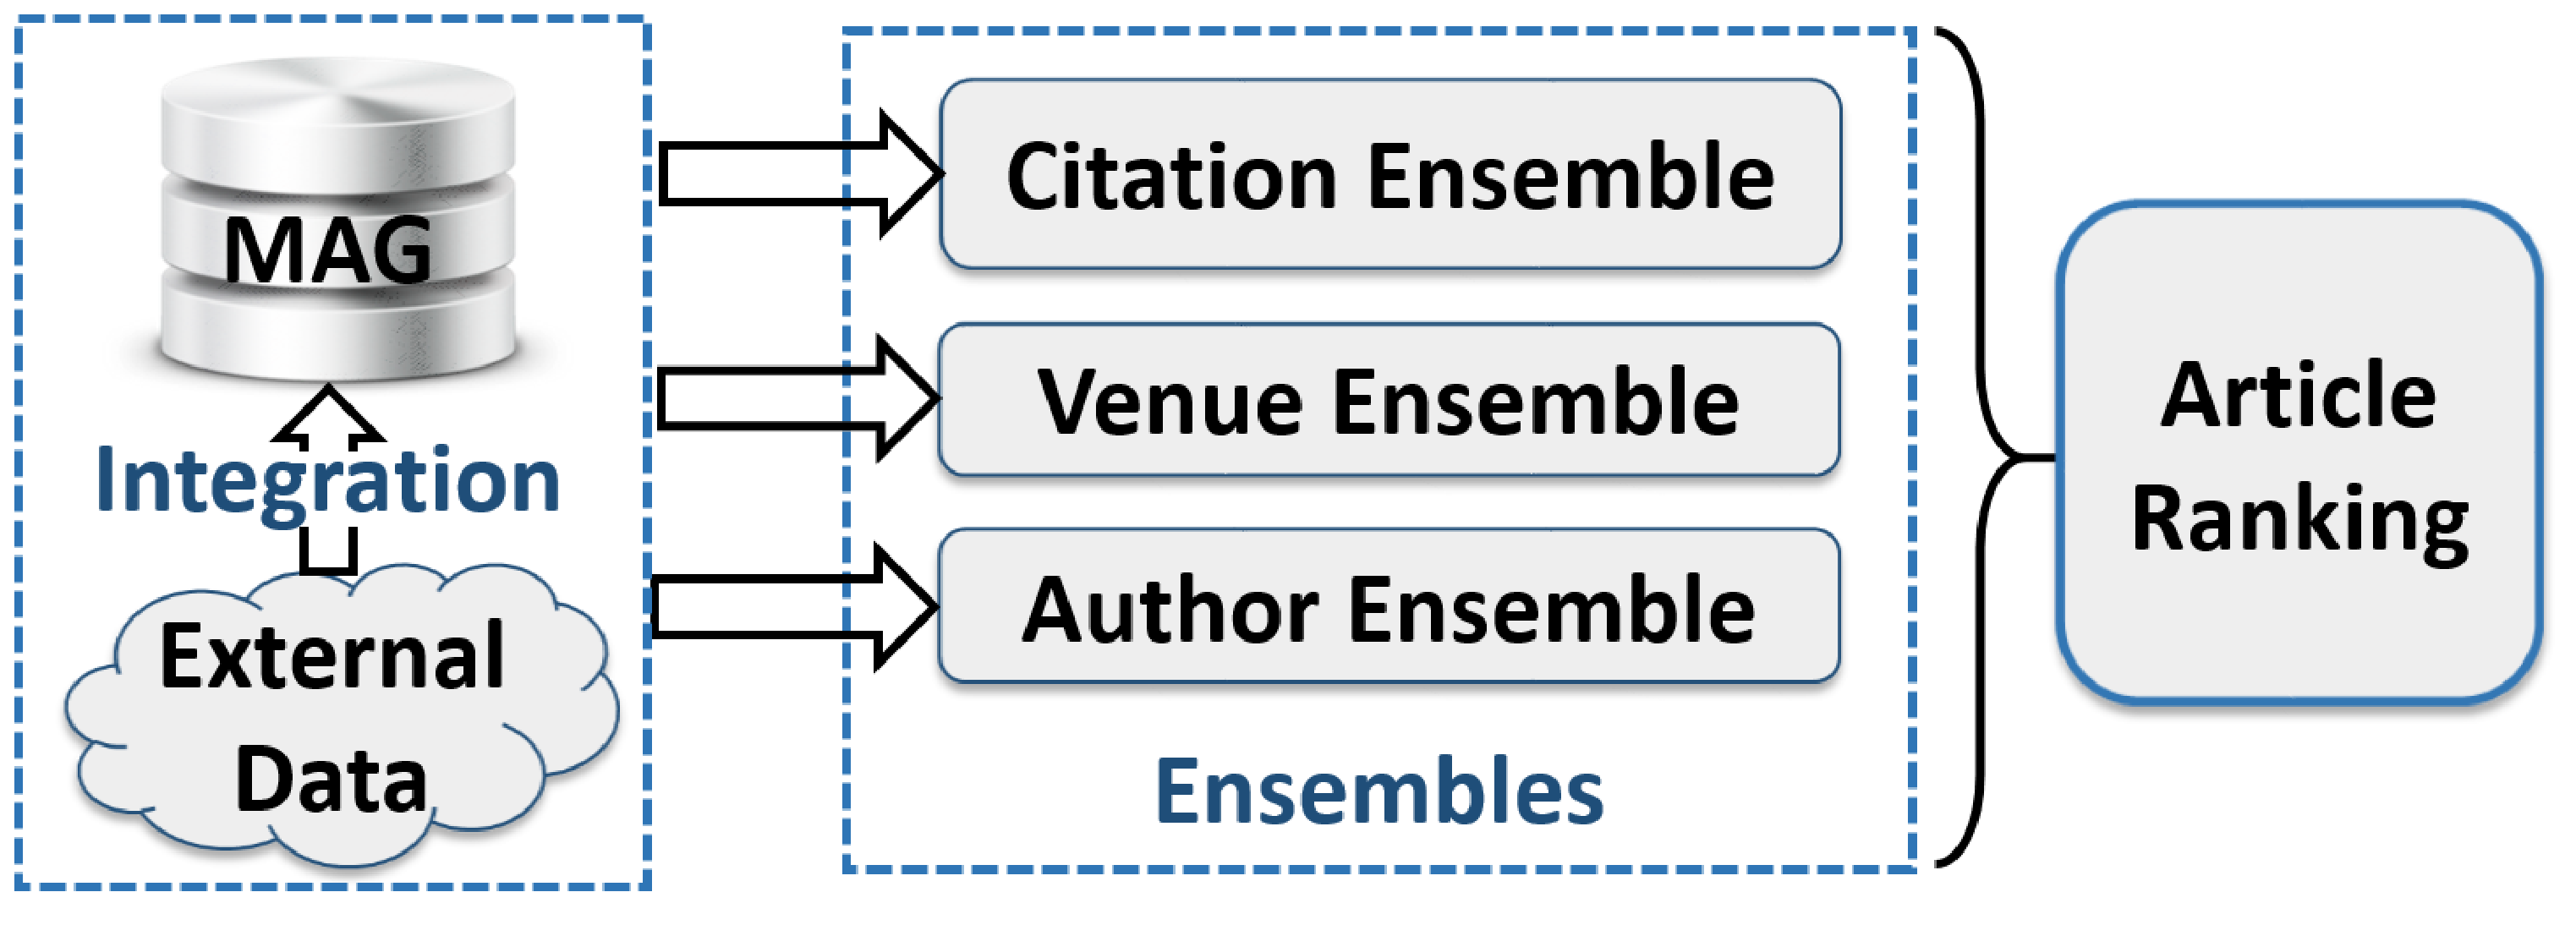
\includegraphics[scale=0.15]{fig/framework.eps}
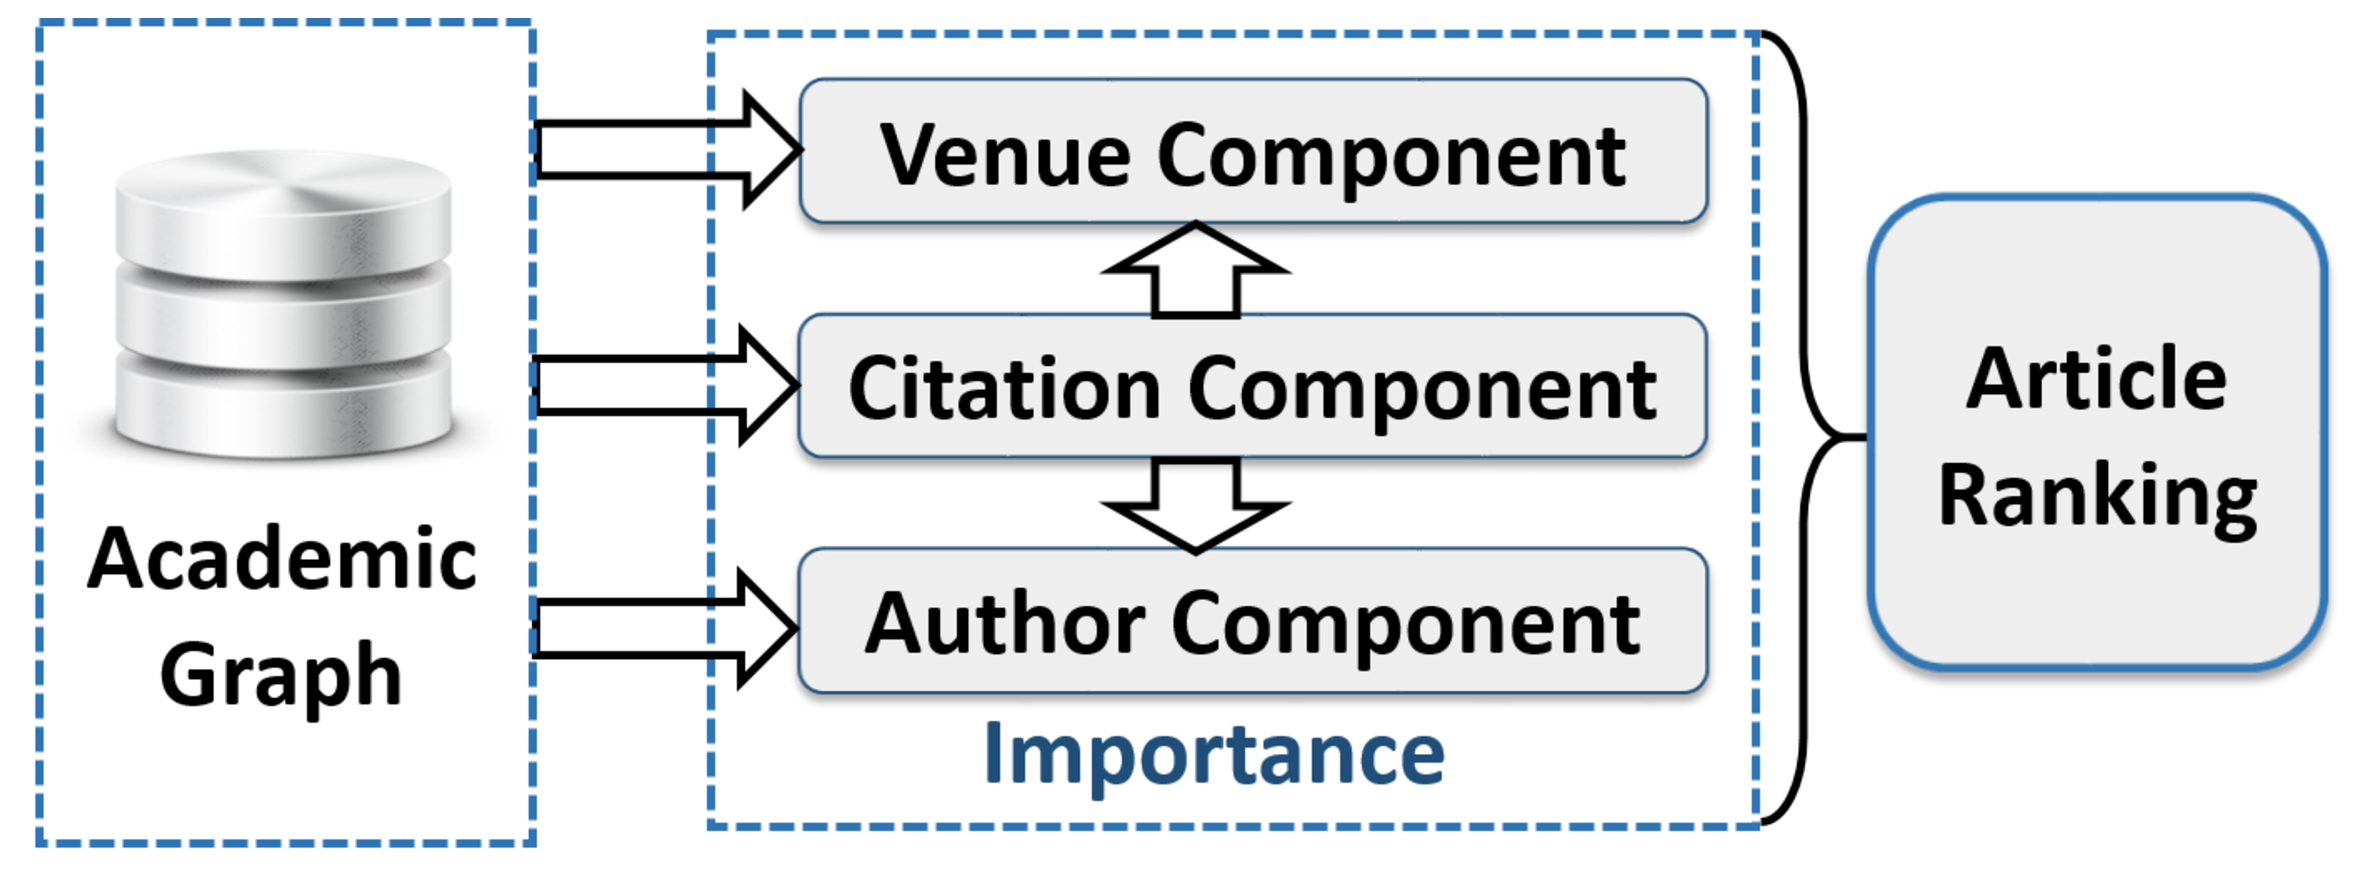
\includegraphics[scale=0.15]{fig/framework-lite-2.eps}
\vspace{-1ex}
\caption{\small Ranking model \ensemblerank} \label{fig-rankmodel}
\vspace{-2ex}
\end{figure}



\stitle{Author component}.
The author component computes the importance of authors with their published articles.

Similar to the venue component, we evaluate the importance of each author, and compute the average importance of the authors of an article as its {\em author importance score}.

However, the resulting author citation graph to compute the prestige is typically too large to handle. Hence, we evaluate the prestige of an author, by using the average prestige of all articles published by the author. Similar to the venue component, the popularity of an author is also defined as the average popularity of her/his published articles. Finally, the prestige and popularity are combined to derive the importance in the same way as the citation component.

%, which can be directly obtained from the citation component,
%to evaluate the authority of that author.

\eat{
\stitle{Affiliation ensemble}.
Recall that articles in our data are also associated with affiliation information. Following the way of the venue or author ensemble, we can derive another ensemble, \ie affiliation ensemble. However, we argue that the use of affiliation ensemble may have negative effects since the correlation between the importance of an article and the average authority of its affiliation(s) is not as strong as others such like authors and venues. As shown by the experimental study in Section~\ref{sec-exp},  the incorporation of the affiliation ensemble impairs the ranking accuracy. Hence, we choose not to use the affiliation ensemble in our model.
}



%\subsection{Ranking with Importance}
%{\label{subsec-eerank}}


\stitle{Ranking with importance assembling}. The aforementioned importance is finally assembled to produce the final ranking, as illustrated in Fig.~\ref{fig-rankmodel}. Before assembling, each component is properly scaled such that the average citation importance score, venue importance score and author importance score
are the same.  Let the scaled importance scores of article $v$ be $R_c(v)$, $R_v(v)$, and $R_a(v)$ from the citation, venue and author components, respectively. The final ranking score $R(v)$ of an article $v$ is aggregated as follows:

\vspace{-2ex}
\begin{small}
\begin{equation} \label{eq-ensemble}
R(v) =  \alpha R_c(v) + \beta R_v(v) + (1 - \alpha - \beta) R_a(v).
\end{equation}
\end{small}
\noindent Here aggregating parameters $\alpha$ and $\beta$ and value $(1 - \alpha - \beta)$ are used to regularize the contributions of the citation, venue and author information. Intuitively, these parameters indicate the intensity of the correlation between the importance of scholarly articles and the specific information.


\stitle{Remarks}.
\marked{It is also possible to train a discriminative model which directly optimizes certain loss functions for ranking, \eg \cite{Richardson06:BPR} for Web pages. Alternatively, this work follows the graph-based formalization, and further develops efficient batch and incremental algorithms based on graphs for scholarly article ranking (Sections~\ref{sec-alg} \& \ref{sec-incAlg}). }

%\subsection{Framework}
%\label{subsec-framework}

%Our ensemble enabled ranking model~\ensemblerank is illustrated in Fig.~\ref{fig-rankmodel}, which contains three distinct ensembles derived from academic graph data, \ie the citation ensemble, venue ensemble and author ensemble. The citation ensemble directly uses TWPageRank, while the other two are partially based on TWPageRank. Moreover, the citation ensemble also helps to derive the venue ensemble and author ensemble. These ensembles are further assembled to produce the final ranking.


%As illustrated in Fig.~\ref{fig-rankmodel}, external data is also exploited in \ewpr. How to collect and use external data will be introduced in the coming section.


\eat{
\stitle{Remarks}.
Traditional PageRank equally distributes the prestige of nodes, and PageRank based models suffer from the problem that older articles are preferred since they have accumulated a large number of citations~\cite{Li08TSRanking}, and TWPageRank based models alleviate the problem to a certain degree by lowering the impact weights of articles when they are cited after their peak time, \ie $T_u\geq Peak_v$. We further propose the venue and author ensembles to improve the ranking accuracy.
}



%\stitle{Remarks}.
%Recall that articles in our data are also associated with affiliation information. Following the way of the venue or author ensemble, we can derive another ensemble, \ie affiliation ensemble. However, we argue that the use of affiliation ensemble may have negative effects since the correlation between the importance of an article and the average authority of its affiliation(s) is not as strong as others such like authors and venues. As shown by the experimental study in Section~\ref{sec-exp},  the incorporation of the affiliation ensemble impairs the ranking accuracy. Hence, we choose not to use the affiliation ensemble in our model.


%our method used for author ensemble is both lightweight and effective, as will be shown in the experimental study.

%Two methods are used to evaluate the authority of venues and authors, respectively. We point out that the ensembles are quite flexible to the selection of these methods, and others may also be incorporated in the ensembles if appropriate.

\eat{
\subsection{Dealing with Missing Data}
\label{subsec-impl}

Data quality is one of the most challenging issues in large scale data management, especially for data from open domains and multiple sources, \eg the Microsoft Academic Graph (MAG)~\cite{Sinha15:MAG}.
The early version of MAG has $120$ million scholarly articles, among which we find that there are about $73$ million articles without references and about $77$ million ones without venues. The ranks of those articles with missing information are underestimated by our model \ewpr, since ensembles assign the minimum scores to articles. As a result, data missing seriously impairs the ranking accuracy.

As for references and venues, the later are easier to obtain, and each filled venue can have a direct and substantial impact on the article ranking, \ie $R_v(u)$ of Eq.~(\ref{eq-ensemble}). In contrast, a filled reference only has an indirect and slight impact. Hence, we decide to use external data to fill in missing venues.


%\subsection{Data Collecting}
%\label{subsec-datacraw}
\stitle{Data collecting}.
The raw external data is collected from publicly available Digital Libraries, such as IEEE Xplore ({\footnotesize http://ieeexplo-re.ieee.org/gateway/}),  PubMed ({\footnotesize http://www.ncbi.nlm.nih.gov/pub-med/}) and DBLP ({\footnotesize http://dblp.uni-trier.de/db/}). In total, we collect $2.8$ million articles with venue information as our external data, in which there are $57,000$ different venues.



%\subsection{Data Preprocessing}
%\label{subsec-dataprep}
\stitle{Data preprocessing}.
The venues in MAG are well processed, and are replaced by their series names. For example, {\em ``9th International Conference on Web Search and Data Mining, 2016''} is replaced with {\em ``Web Search and Data Mining''}. This makes it hard to directly link with the collected raw venue names. Hence, we preprocess raw venue names for the simplification of subsequent venue linking.
%
We first remove stop words such as {``on''} and common words like {``Conference''}, as well as years and some special characters from collected raw venue names. Then the same venues are merged, and the number of different venue names is reduced to $42,000$.

%\subsection{Data Linking}
%\label{subsec-datamap}
\stitle{Data linking}.
The final and also the most important step of filling missing venue information is to link each collected venue name to an existing one in MAG. Intuitively, linking based on name similarity is the most effective way such that two venues are linked if their names bear high similarity. We exploit the Jaro metric to evaluate the name similarity, which is based on the number and order of the common characters between two strings, and obtains good results in tasks such as record linkage and name matching~\cite{Cohen03strcompa}. Formally, a collected venue name is linked to an existing one in MAG if their Jaro similarity exceeds a pre-define threshold.

However, such a threshold is nontrivial to determine in practice. A high threshold can guarantee the accuracy of linked pairs, while only a tiny proportion of collected venue names are linked. On the other hand, a low threshold increases the number of linked pairs, which, in the same time, also introduces many errors. In order to reach a good balance between the number of linked pairs and the accuracy, we propose to combine another constraint on topic similarity of venues for linking, and only weaker filter conditions need be used in both constraints.

In MAG, fields of study (FOS) represent research topics of articles, such as {\em Web pages}, and {\em language technology}. Hence, we use FOS to evaluate the topic similarity of two venues. There are about $54,000$ FOS in MAG and most articles are assigned with two or three FOS. Let the set of FOS of each venue be the union of the sets of FOS of articles published in that venue. And the topic similarity of two venues based on FOS is defined as:
\begin{small}
\begin{equation} \label{eq-fos}
TS(s,t)=({|F_s\bigcap F_t|})/{\sqrt{|F_s|\cdot|F_t|}},
\end{equation}
\end{small}
\noindent in which $s$ and $t$ are two venues, and $F_s$ and $F_t$ are the sets of FOS of $s$ and $t$, respectively.

When we link a collected venue name, it is directly linked to the most similar one in terms of name similarity, if their Jaro similarity exceeds a high threshold $\lambda$. Otherwise, we first use the topic similarity constraint to select several candidates in MAG, \ie venues whose topic similarities with the collected venue exceed a threshold $\theta$. Intuitively, these candidates are in the similar fields of the collected one. We then select the most similar candidate in terms of name similarity as its linked venue, if their Jaro similarity exceeds another threshold $\phi$. Hence, the collected venue is linked to the one to which it is similar in terms of both topics and names.

In our model \ewpr, threshold $\lambda$ is set to $0.95$, while thresholds $\theta$ and $\phi$ need not be very high, which are $0.5$ and $0.7$, respectively. Finally, $6,000$ among the $42,000$ collected venues are linked, resulting in $340,000$ (about $12\%$) articles with enriched venue information. Note that a majority of the collected venue names are not valid venues, such as booktitles and names of workshops, and cannot be linked to any one in MAG.
}



\subsection{Algorithm}

With emission probabilities and transition probabilities estimated from Equations
\ref{equ:emi-prob} and \ref{equ:trans-prob}, we can use the Viterbi algorithm to
compute the optimal path. The Viterbi algorithm is a dynamic programming
algorithm that can quickly detect a sequence of states that maximizes the joint
probability, which is the product of the emission probabilities and transition
probabilities of all the states in the sequence. The detected sequence is the
path with maximum likelihood and thus the global optimal path.



\begin{large}
\begin{algorithm}
\caption{The CT-MM Algorithm}\label{alg:viterbi}
\small
\begin{algorithmic}[1]
 \State  \textbf{Input}: $\overline{\mathcal{T}}$,$\epsilon$,G(V,E)
 \State  \textbf{Output}: map matching result R

 \State $E_1 \gets findCand(G(V,E),p_1)$.

 \State \textbf{Initialize} $f[r_1^k] = p(r_{1}^k|p_{1}), k = 1,2,\cdots,10$.

 % \For{each line segments in $\overline{\mathcal{T}}$}
 \For{$i = 2 \to n$}
   % \State extract candidate set of that GPS point from road network.
   \State $P_i \gets \overline{\mathcal{T}}[i].e$
   \State $P_{i-1} \gets \overline{\mathcal{T}}[i].s$
   \State $E_i \gets findCand(G(V,E),P_i)$.\Comment{find candidate set}
   % \State extract subgraph between the previous and current GPS point.
   \State $G_s \gets extract(G(V,E),\overline{\mathcal{T}}[i],\epsilon)$.
   \Comment{extract subgraph}
   \For{$r_i^j \in E_i$}
      \State compute $p(r_{i}^j|P_{i})$ by equation (6)
      \State $f[r_{i}^j] = -\infty$
      \For{$r_{i-1}^k \in E_{i-1}$}
      % \State compute shortest path from $r_{i-1}$ to $r_{i})$ in the sub action graph.
      % \State $sp_i^j\gets shortestPath(r_{i-1},r_{i},sbGraph)$
      \State $R_{j,k} \gets PathRec(G_s,r_i^j,r_{i-1}^k)$.\Comment{path recovery}
      \State compute $p(r_{i-1}^k,r_{i}^j)$ by equation (7)
      \State $Conj\gets f[r_{i-1}^j] * p(r_{i-1}^j,r_{i}^k) * p(r_{i}^j|P_{i})$
      \If{$Conj \ge f[r_{i}^k]$}
        \State $f[r_{i}^k] = Conj$
        \State $Pre[r_{i}^k] = r_{i-1}^j$
      \EndIf
    \EndFor
  \EndFor
  \EndFor
  \State $R = \argmax_{r_1^{k_1}\rightarrow r_2^{k_2}\rightarrow \cdots \rightarrow r_n^{k_n}}f[r_{n}^{k_n}]$
\State \textbf{return} $R$\Comment{The matched result is R}

% \Procedure{getSubGraph}{$p_{i-1},p_i,length,width$}
% \State get bounding box.
% \EndProcedure
\end{algorithmic}
\end{algorithm}
\end{large}


\section{Dynamic Ranking Computation}
\label{sec-incAlg}

Scholarly articles are dynamic and continuously growing, and it is impractical to recompute ranking from scratch once they get updated. In this section, we present an incremental algorithm for our ranking model \ensemblerank.


\subsection{Incremental Algorithm Framework}
\label{subsec-inc-alg}




Our incremental algorithm \incensemble incrementally computes the popularity and prestige of scholarly articles.
We consider that an update $\Delta$ = $\Delta V\cup\Delta E$ is added to a   (citation or venue) graph $G(V, E)$,
and the resulting graph is $G^+(V\cup\Delta V, E\cup\Delta E)$, where
$\Delta V$ is a set of nodes with $\Delta V\cap V = \emptyset$, and $\Delta E$ is a set of directed edges on $\Delta V$ and from $\Delta V$ to $V$ only, as article citation relationships obey a natural temporal order, \ie an article only cites those published earlier, and it is rare for the mutual citations between two articles published in the same time.


\stitle{Incremental popularity computation}.
The popularity of venues and authors is computed along the same lines as their batch counterparts of algorithm \batensemble,
as almost all venues and authors are affected  by the definitions of the popularity of venues and authors.


As the popularity of articles is defined as the freshness sum of all their citations, it is convenient to maintain in a dynamic scenario. Consider an updated citation graph $G^{c,+}(V^c\cup\Delta V^c, E^c\cup\Delta E^c)$ of $G^c(V^c, E^c)$, and the updated popularity $Pop_{c}^+(v)$ can be computed as:

\vspace{-1ex}
\begin{small}
\begin{equation}\label{eq-inc-pop}
Pop_c^+(v) = Pop_c(v) {e^{\sigma (T^+_0-T_0)}} + \sum_{(u,v)\in \Delta E^c} {e^{\sigma (T^+_0-T_u)}},
\end{equation}
\end{small}
\noindent
where $Pop_c(v)$ (resp. $Pop_c^+(v)$) is the popularity of node $v$ on $G^c$ (resp. $G^{c,+}$), and
 $T_0$ (resp. $T^+_0$) is the current time in $G^c$ (resp. $G^{c,+}$).
%
By Eq.~(\ref{eq-inc-pop}), it is easy to see that it takes $O($ $|V^c|+|\Delta V^c|+|\Delta E^c|)$ time to update the popularity.
%This further shows that Eq.~(\ref{eq-inc-pop}) is a desired solution for popularity maintenance.



\stitle{Incremental prestige computation}.
The prestige of authors is computed along the same lines as the batch algorithm \batensemble,
as almost all authors are affected  by the definition of the prestige of authors.
%
For articles and venues, we propose an incremental algorithm to maintain their prestige.



%We first present the incremental  prestige computation. Again, it differs for the prestige of articles and venues in a specific year and the one of authors. We finally present the complete incremental algorithm \incensemble, which is similar to the batch algorithm \batensemble, except that (1) it uses algorithm \inctwprscc to incrementally compute the prestige of articles and venues, and (2) it incrementally computes the popularity of articles based on Eq.~(\ref{eq-inc-pop}).




\subsection{Incremental TWPageRank Computation}
\label{subsec-incTWPageRank-computation}

%\subsubsection{Prestige of articles and venues in a specific year}
%\label{subsubsec-incprs-CV}
%\subsubtitle{Prestige of articles and venues in a specific year}.
%We expand $M$ and $PR$ to the same sizes as $M^+$ and $PR^+$, respectively, by filling zeros, and let $\Delta M=M^+ - M$ and $\Delta PR = PR^+ - PR$.




Consider a citation or venue graph $G(V, E)$, its TWPageRank vector $PR$ and the topological order $O$ of its block-wise graph. Given an update $\Delta$ = $\Delta V\cup\Delta E$ to $G$, the incremental prestige computation for articles and venues in a specific year is to compute the TWPageRank vector $PR^+$ on the updated graph $G^+(V\cup\Delta V, E\cup\Delta E)$.


\stitle{Auxiliary data structure maintenance}.
Two auxiliary data structures in the batch algorithm~\twprscc need to be maintained : (a) on the block-wise graph,  a mapping that, given a node of graph $G$, returns the index of the \scc to which it belongs, and (b) the topological order of the nodes in the block-wise graph.
%
Observe that these auxiliary data structures can be easily maintained as follows.

%the idea is to divide $G$ into affected and unaffected areas such that TWPageRank scores of nodes in affected and unaffected areas are updated accordingly.


\sstab(1) The block-wise graph of $G^+$ needs to be computed, whose \sccs consist of the \sccs in $G$ and \sccs in the induced subgraph $G^+[\Delta V]$, as  the edges of $\Delta E$ are  on nodes in $\Delta V$ and from $\Delta V$  to $V$ only. Hence, only those new \sccs in $G^+[\Delta V]$ need to be computed.

\sstab(2) The updated topological order $O^+=\Delta O/O$, where $\Delta O$ is the topological order of the block-wise graph of induced subgraph $G^+[\Delta V]$. Hence, only $\Delta O$ needs to be computed. One can easily verify the following.


\begin{prop} \label{lemma-inc-topo}
 $O^+=\Delta O/O$ is indeed a valid topological order of the block-wise graph of $G^+$.
\end{prop}

\begin{proofSketch}
We prove that for each edge $(u,v)$ in the block-wise graph of $G^+$, node $u$ comes before $v$ in $O^+$, and the conclusion follows by the definition of topological order.
\end{proofSketch}

\eat{
\begin{proof}
Let $E'_c$ denote the set of cross edges from $V'_\Delta$ to $V'$.
It suffices to show that for each $(u,v)\in E'\cup E'_\Delta \cup E'_c$, $u$ comes before $v$ in $O^+$,
which obviously holds (1) for  $E'\cup E'_\Delta$ as $O$ and $\Delta O$ are topological orders of $G'$ and $G'_\Delta$, respectively, and (2) for $E_{c}'$ as nodes in $G'_\Delta$ come before nodes in $G'$.
\end{proof}
} %%%%%%%%%% for eat


%%%%%%%%%%%%%%%%%%%%%Algorithm
\begin{figure}[tb!]
%\vspace{2ex}
\begin{center}
{\small
\begin{minipage}{3.36in}
\myhrule \vspace{-1.5ex}
\mat{0ex}{
%%%%%%%%%%%%%%%%%%%
{\sl Input:\/} \= An update $\Delta$ = $\Delta V\cup\Delta E$, TWPageRank vector $PR$ of $G$,\\
\hspace{5ex}   and the  topological order $O$ of the block-wise graph $G'$.\\
{\sl Output:\/} TWPageRank vector $PR^+$ of the updated graph $G^+$. \\
\bcc \hspace{1.5ex}\=  $G_C'$ := the block-wise graph of $G_C$; \\
%\ \  $E_{CB}'$ := edges from $G_C'$ to $G'$\\
\icc\> $\Delta O$ := topological order of $G_C'$; \ \ $O^+$ := $\Delta O/O$; \\
\icc\> label \sccs of $G_C$ as $C$ and \sccs of $G$ with outgoing edges \\ \hspace{2.5ex}  having  weight changes as $B$,  the remaining \sccs of $G$ as $A$\\
\icc\>  \For each node $v'$ following $O^+$ \Do\\
\icc\>\hspace{2.5ex}\= $scc$ := the corresponding \scc of $v'$; \\
%\icc\>\>\If impact weight of $(v,w)$ is changed where $v\in scc$ \Then \\
%\icc\>\>\hspace{3ex}\= label $scc$ as $B$;\\
%\icc\>\>\> label SCC $w'$ as $B$ such that $(v',w')\in E'$; \\
\icc\>\> \If $scc$ is labeled as $C$ \Then \\
\icc\>\>\hspace{3ex}\= update $PR^+(v)$ ($v\in scc$) following algorithm~\twprscc; \\
\icc\>\>\> label \scc $w'$ as $B$ with $w'\in G'$ and $(v', w')\in E^+{'}$;\\
\icc\>\> \Else \If $scc$ is labeled as $B$ \Then \\
\icc\>\>\> update $PR^+(v)$ where $v\in scc$ with Eq.~(\ref{eq-inc-prscc}) until the \\ \hspace{8ex}  sum of TWPageRank score changes is less than $\epsilon\cdot \frac{|scc|}{|V^+|}$; \\
\icc\>\>\> label \scc $w'$ as $B$ with $(v',w')\in E'$;\\
\icc\>\> \Else $PR^+(v)$:=$PR(v)\cdot {n}/{n^+}$ where $v\in scc$; \\
\icc\> \Return $PR^+$.
}
\vspace{-2.5ex} \myhrule
\end{minipage}
}
\end{center}
\vspace{-2ex}
\caption{\small Algorithm~\inctwprscc for incremental TWPageRank} \label{alg-inctwprscc}
\vspace{-3ex}
\end{figure}
%%%%%%%%%%%%Algorithm

%%% affected/unaffected division
\stitle{Analyses of affected and unaffected areas}.
The TWPageRank vector $PR$ of graph $G$ is mainly affected in two ways.



\sstab(1) Let $V_{B,1}\subseteq V$ be the set of nodes reachable from the newly added nodes $\Delta V$, $V_{B,2}\subseteq V$ be the set of nodes with outgoing edges having weight changes, and $V_{B,3}\subseteq V$ be the set of nodes reachable from  $V_{B,2}$.
%
Then $V_B=V_{B,1}\cup V_{B,2}\cup V_{B,3}$ is obviously the set of nodes in $G$ affected by the update $\Delta$.
%
TWPageRank scores on $V_B$ are re-iterated as follows, where notations with superscript `$+$' are defined on  $G^+$.
%using the existing TWPageRank vector scaled with constant ${n}/{n^+}$.

\vspace{-2ex}
\begin{scriptsize}
\begin{equation}\label{eq-inc-prscc}
\begin{split}
PR^+(v) \ = \ &  d \sum_{(u,v)\in E^+_i} M^+_{u,v} PR^+(u) + d \sum_{(u,v)\in E^+_a} M^+_{u,v} PR^+(u)  \\
 + \frac{n}{n^+} \Big( PR(v) &  - d \sum_{(u,v)\in E_i} M_{u,v} PR(u) - d\sum_{(u,v)\in E_a} M_{u,v} PR(u)\Big).
\end{split}
\end{equation}
\vspace{-2ex}
\end{scriptsize}


\sstab(2) Let $V_A = V\setminus V_B$. Since nodes in $V_A$ are not reachable from newly added or affected nodes, $V_A$ is essentially not affected by the update $\Delta$. And TWPageRank scores on $V_A$ only need to scale with constant ${n}/{n^+}$.

Let $G_A=(V_A,E_A)$, $G_B=(V_B,E_B)$ and $G_C=(V_C,E_C)$, respectively, and
let $E_{AB}$ and $E_{CB}$  be the sets of edges from $G_A$ to $G_B$ and from $G_C$ to $G_B$, respectively.
In this way, graph $G^+$ is divided into subgraphs $\{G_A$, $G_B$, $G_C\}$ and edge sets $\{E_{AB}, E_{CB}\}$.
%
We then have $G_C$ = $G^+[\Delta V]$, $\Delta E$ = $E_C\cup E_{CB}$, $V$ = $V_A\cup V_B$ and $E$ = $E_A\cup E_B\cup E_{AB}$.



\stitle{Incremental algorithm \inctwprscc}. We now present our incremental algorithm for TWPageRank, shown in Fig.~\ref{alg-inctwprscc}.


It takes as input an update $\Delta$ and the previous results on the original graph $G(V, E)$, and returns the TWPageRank vector of the updated graph $G^+$. It first incrementally computes the topological order $O^+$
%by concatenating the topological orders of $G_C'$ and $G'$
(lines 1--2). %Note that $G_C'$ is the same to $G'_\Delta$.
%
After that, it labels the newly added \sccs with $C$ and existing \sccs with $A$ or $B$, depending on whether the existing \sccs have weight changes on outgoing edges (line 3).
%
It then processes each \scc in the order $O^+$ such that the TWPageRank scores of nodes in each \scc are updated according to the labels (lines 4--12), and finally returns the TWPageRank vector (line 13).
%
%More specifically, the scores of nodes in SCCs labeled as $C$ and $B$ are updated the same to Algorithm~\twprscc, while the scores of nodes in SCCs labeled as $A$ are simply scaled.
%
%It is also easy to verify that nodes in SCCs labeled as $A$, $B$ and $V$ corresponding to $V_A$, $V_B$ and $V_C$.

When processing $V_B$ with Eq.~(\ref{eq-inc-prscc}), {\em edges in $E_{AB}$ can be skipped}  since $PR^+(u)={n}/{n^+}\cdot PR(u)$ for $u\in V_A$ and $M_{u,v}=M^+_{u,v}$ for $(u,v)\in E_{AB}$. Besides, we use ${n}/{n^+}\cdot PR$ as the initial vector. Both of them can speed up the computation.


\eat{
\begin{figure}[tb!]
\centering
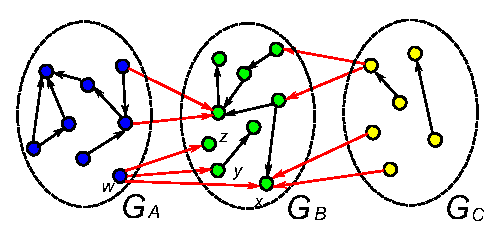
\includegraphics[scale=0.6]{fig/General_framework_peak_ABC.eps}
\vspace{-3ex}
\caption{\small An example of affected and unaffected areas}
\label{fig-inc-division}
\vspace{-3ex}
\end{figure}

\begin{example} \label{eg-layer-dag}
Figure~\ref{fig-inc-division} illustrates an example of affected and unaffected areas, in which subgraphs $G_A$, $G_B$ and $G_C$ are associated with node sets $V_A$, $V_B$ and $\Delta V$, respectively. Here the citation peak time of node $x$ is changed, which leads to the changes of the normalized weights of edges $(w,x)$, $(w,y)$ and $(w,z)$.
\end{example}
}


\begin{figure}[tb!]
\centering
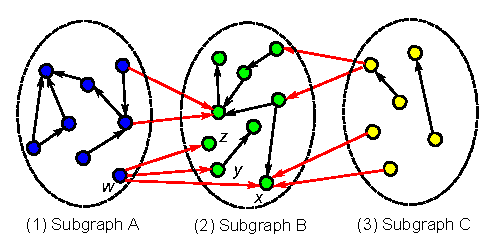
\includegraphics[scale=0.7]{fig/General_framework_peak.eps}
\vspace{-2ex}
\caption{\small An example of incremental TWPageRank computation}
\label{fig-inc-division}
\vspace{-4ex}
\end{figure}

\begin{example} \label{eg-layer-dag}
Figure~\ref{fig-inc-division} illustrates an example of incremental TWPageRank computation. Consider an update $\Delta$ on the original graph $G$.
%
It is obvious that the update $\Delta$ has no impacts on the SCCs of $G$, and $O^+$ defined earlier is a valid topological order of $G^+{'}$.
%
The original graph $G$ is then partitioned into affected and unaffected areas, and subgraphs $G_A$, $G_B$ and $G_C$ are associated with node sets $V_A$, $V_B$ and $\Delta V$, respectively. Here edge weight on $(y, x)$ changes due to the change of the citation peak time of node $x$, and, hence, node $y$ as well as all nodes reachable from $y$ are included in $G_B$.
%
When updating the TWPageRank scores, following $O^+$, scores of nodes in $G_C$, $G_B$ and $G_A$ are computed by iterations from scratch, by iterations with Eq.~(\ref{eq-inc-prscc}) using the existing TWPageRank vector and by scaling, respectively.
\end{example}

\vspace{-1ex}
\begin{theorem}
\label{lemma-subgraphA}
The TWPageRank vector $PR^+$ returned by~\inctwprscc converges such that $||PR^+-PR^{*}||_1 < \epsilon$, where $PR^{*}$ is the convergent TWPageRank vector.
\end{theorem}


\begin{proofSketch}
Assume a topological order $v_1'/\dots/v_{l}'$ of the block-wise graph $G^+{'}$ where $l=|O^+|$. It suffices to prove by induction that the sum of changes of $PR^+(v)$ ($v\in scc_k$) is no more than $\epsilon |scc_k|/|V^+|$ for $scc_k$ of $v_k'$ ($k\in [1,l]$).
%The conclusion follows combining Lemma~\ref{prop-prscc}
%(see \cite{SARank-full} for details).
\end{proofSketch}




Observe that (a) a topological order of $G'_C$ can be computed in $O(|V_C|+|E_C|+|E_{CB}|)$ time,
(b) updating the TWPageRank scores of nodes in subgraphs $G_B$ and $G_C$ costs $O(|V_B\cup V_C|+|E_{B,a}\cup E_{C,a}\cup E_{CB}|)+t^+|E_{B,i}\cup E_{C,i}|)$ time, and , finally, (c) updating the scores of nodes in $G_A$ costs $O(|V_A|)$ time. From these, the following holds.


\begin{prop} \label{lemma-inc-citation-comp}
Given an update $\Delta$ = $\Delta V\cup\Delta E$ of citation or venue graph $G(V,E)$, the TWPageRank vector of $G$ and the topological order of $G'$, algorithm \inctwprscc runs in $O(|V\cup \Delta V| + |E_B\cup E_C\cup E_{CB}| + t^+|E_{B,i}\cup E_{C,i}|)$ time.
\end{prop}



%Note that the incremental algorithm reduces the complexity of updating subgraph $A$ from $O(|E^c_A|)$ to $O(|V^c_A|)$. It is more effective when only a small number of articles are updates, resulting in $|V^c_A|>>|V^c_B|+|V^c_C|$ and updating subgraph $A$ occupies most of the computation.

By Propositions~\ref{prop-converg} \& \ref{lemma-inc-topo} and Theorem \ref{lemma-subgraphA}, one can easily verify the correctness of algorithm \inctwprscc.
%
Note that  a) algorithm \inctwprscc computes \sccs and derives the topological order based  on $\Delta$ only, instead of $G^{+}$,
b) it skips edges in $E_A\cup E_{AB}$ when updating the scores of nodes in $G_A$ and $G_B$, and
c) the number $t^+$ is very likely smaller than the number $t$ of \twprscc when updating scores of nodes in $G_B$.
%
All these make \inctwprscc faster than \twprscc even though they have very similar time complexity.
%, as will also been shown by the experimental study,



%%%%%%%%%%%%%%%%%%%%%%%%%%%%%%%%%%%%%%%%%%%%%%%%%%
\begin{table}[tb!]
%\vspace{-2ex}
\begin{center}
\caption{\small Statistics of affected/unaffected areas given a yearly update, \ie articles of 2011 on \aan and 2015 on \aminer and \magdata, respectively.}
\label{tab-inc}
\begin{small}
\vspace{-.5ex}
\eat{
\begin{tabular}{|c|c|c|}
\hline
{\bf Graphs} & $|V_A|$\hspace{2ex}$|V_B|$\hspace{3ex}$|V_C|$ & $|E_A|$\hspace{2ex}$|E_{AB}|$\hspace{2ex}$|E_B|$\hspace{2ex}$|E_{CB}|$\hspace{2ex}$|E_C|$ \\
\hline \hline
% citation graphs
\aan & $46.9\%$\ $47.3\%$\ $5.8\%$ & \ $2.9\%$\ $25.9\%$\ $60.5\%$\ $10.4\%$ \hspace{1ex} $0.3\%$ \\
\aminer & $81.4\%$ \hspace{1ex} $10.7\%$ \hspace{1ex} $7.8\%$ & $18.0\%$ \hspace{1ex} $53.2\%$ \hspace{1ex} $25.1\%$ \hspace{1ex} \ $2.3\%$ \hspace{1ex} $1.4\%$ \\
\magdata & $69.5\%$ \hspace{1ex} $25.9\%$ \hspace{1ex} $4.5\%$ & \ $1.0\%$ \hspace{1ex} $27.4\%$ \hspace{1ex} $64.5\%$ \hspace{1ex} \ $7.0\%$ \hspace{1ex} $0.1\%$ \\ \hline
% venue graphs
\aan & \ $2.1\%$ \hspace{1ex} $92.0\%$ \hspace{1ex} $5.8\%$ & \ $1.0\%$ \hspace{1ex} \ $1.0\%$ \hspace{1ex} $88.8\%$ \hspace{1ex} $10.0\%$ \hspace{1ex} $0.2\%$ \\
\aminer & $45.8\%$ \hspace{1ex} $47.7\%$ \hspace{1ex} $6.4\%$ & \ $0.0\%$ \hspace{1ex} \ $3.2\%$ \hspace{1ex} $95.4\%$ \hspace{1ex} \ $1.0\%$ \hspace{1ex} $0.1\%$ \\
\magdata & $12.4\%$ \hspace{1ex} $84.6\%$ \hspace{1ex} $3.0\%$ & \ $0.0\%$ \hspace{1ex} \ $0.1\%$ \hspace{1ex} $92.6\%$ \hspace{1ex} \ $7.1\%$ \hspace{1ex} $0.1\%$ \\
 \hline
\end{tabular}
}
\begin{tabular}{|r|c c c|c c c|}
\hline
 & \multicolumn{3}{c|}{\bf Citation graphs on}   & \multicolumn{3}{c|}{\bf Venue graphs on}    \\
\raisebox{1ex}[0pt]{\bf Statis.} & \aan & \aminer & \magdata & \aan & \aminer & \magdata \\
\hline \hline
$|V_A|$ & 47.4\% & 52.3\% & 69.2\% & 2.1\% & 8.7\% & 12.4\% \\
$|V_B|$ & 46.8\% & 40.0\% & 26.3\% & 92.0\% & 84.8\% & 84.6\% \\
$|V_C|$ & \ 5.8\% & \ 7.8\% & \ 4.5\% & \ 5.8\% & \ 6.4\% & \ 3.0\% \\ \hline
% venue graphs
$|E_A|$ & \ 3.0\% & 2.4\% & \ 0.9\% & \ 0.0\% & \ 0.0\% & \ 0.0\% \\
$|E_{AB}|$ & 26.5\% & 30.2\% & 26.6\% & \ 1.2\% & \ 0.2\% & \ 0.1\% \\
$|E_B|$ & 59.8\% & 59.3\% & 65.5\% & 88.6\% & 92.3\% & 92.6\% \\
$|E_{CB}|$ & 10.4\% & \ 7.2\% & \ 7.0\% & 10.0\% & \ 7.3\% & \ 7.1\% \\
$|E_C|$ & \ 0.3\% & \ 0.9\% & \ 0.1\% & \ 0.2\% & \ 0.2\% & \ 0.1\% \\ \hline
\end{tabular}
\end{small}
\end{center}
\vspace{-6ex}
\end{table}
%%%%%%%%%%%%%%%%%%%


\stitle{Time \& space complexity analyses of the incremental algorithm}.
By the analyses above, the time complexity of \incensemble is the same as \batensemble, except that \incensemble saves $O(|E^c_A\cup E^c_{AB}|)$ and $O(|E^v_A\cup E^v_{AB}|)$ time on the updated citation and venue graphs. And its space complexity is also the same as \batensemble, except that it uses $(|V^c\cup \Delta V^c|+|V^v\cup\Delta V^v|)$ extra space to store the affected/unaffected areas and $(|E^c\cup \Delta E^c|+|E^v\cup \Delta E^v|)$ extra space to store the original edge weights before update.

Despite of its similar time complexity to \batensemble, algorithm \incensemble typically achieves a substantial efficiency improvement over \batensemble, according to our statistics of affected/unaffected areas shown in Table~II.
%
(a) It saves $O(|V^c|+|E^c|)$ and $O(|V^v|+|E^v|)$ time when maintaining \sccs and the topological order based on $\Delta^c$ and $\Delta^v$ only, where ($|V^c|$, $|E^c|$, $|V^v|$, $|E^v|$) are more than (92\%, 89\%, 93\%, 89\%) of ($|V^{c,+}|$, $|E^{c,+}|$, $|V^{v,+}|$, $|E^{v,+}|$) on all tested graphs;
(b) It saves $O(|E^c_A \cup E^c_{AB}|)$ time when updating scores on $V^c$, where edges in $E^c_A\cup E^c_{AB}$ account for more than 28\% of total edges;
(c) It saves $O(|E^c|)$ time when computing popularity of articles, which accounts for more than 89\% of $|E^{c,+}|$;
And, finally, (d) It is likely to compute TWPageRank scores on $V^c_B$ and $V^v_B$ with less iterations.








\section{Experimental Study}
\label{sec-exp}

In this section, we present an extensive experimental study of our approach \ensemblerank, compared with competitive methods.
Using three real-life scholarly datasets (\aan, \aminer and \magdata) and two sets of ground-truth (\recom and \fcita), we conducted four sets of experiments to evaluate: (1) the effectiveness of \ensemblerank,
%two sets of benchmark article pairs (\recom and \fcita) ranked by numbers of recommendations and future citations,
(2) the efficiency of our batch algorithm \batensemble and incremental algorithm \incensemble, and (3) the impacts of parameters. %\ie time decaying factor $\sigma$, importance weighting factor $\lambda$ and aggregating parameters $\alpha$ and $\beta$.

\subsection{Experimental Settings}

We first present the settings of our experimental study.

\eat{
%%%%%%%%%%%%%%%%%%%%%%%%%%%%%%%%%%%%%%%%%%%%%%%%%%
\begin{table}[t!]
%\vspace{-2ex}
\label{tab-statistics}
\begin{center}
\begin{scriptsize}
\vspace{1ex}
\begin{tabular}{|c|c|c|}
\hline
{\bf Entity / Relation}       &  {\bf Quantity in Phase~1}     & {\bf Quantity in Phase~2} \\
\hline\hline
Paper      &  $122,675,085$       &  $120,887,833$ \\ \hline
Author      &  $123,017,488$       &  $119,892,201$ \\ \hline
Venue      &  $24,841$       &  $24,843$ \\ \hline
Affiliation      &  $2,716,493$       &  $19,849$ \\ \hline
Fields of study     &  $53,834$       &  $53,830$ \\ \hline
Reference      &  $757,462,733$       &  $952,364,264$ \\ \hline
P-A      &  $324,948,062$       &  $312,034,259$ \\ \hline
P-V      &  $45,783,880$       &  $45,290,168$ \\ \hline
\end{tabular}
\vspace{-5ex}
\end{scriptsize}
\end{center}
\caption{Statistics of MAG}
\vspace{-3ex}
\end{table}
%%%%%%%%%%%%%%%%%%%
}

\stitle{Datasets}. We chose three datasets to test our approach.

\noindent
(1) \aan records the collection of computational linguistics articles published at ACL conferences from the year of 1965 to 2011~\cite{Liang16AAAI}.
It contains 18,041 articles, 14,386 authors, 273 venues and 82,944 citations.

\noindent
(2) \aminer records articles in the computer science domain from 1936 to 2016~\cite{Tang:08KDD}.
It contains 3.14 million articles, 1.74 million authors, 11,619 venues and 6.38 million citations.

\noindent
(3) \magdata records articles of various disciplines from 1800 to 2016~\cite{Sinha15:MAG}.
It contains around 127 million articles, 115 million authors, 24,024 venues and 529 million citations.
%Please refer to~\cite{Sinha15:MAG} for more details about \magdata.

\marked{The average number of citations on \aminer is much less than the other two, we hence added part of the missing citations by title matching on \magdata, and, finally, the total number increased to 14.26 million.}
These datasets were further cleaned by deleting self-citations and citations from old articles to new ones, which accounted for (0.1\%, 0.8\%, 0.4\%) of the total citations on (\aan, \aminer, \magdata), respectively.
%from old articles to more recent ones
%These datasets were further cleaned by detecting citation cycles and removing those edges violating the temporal order if any.

%The original datasets does not strictly follow the temporal order due to the data quality problem. We hence dealt with the issuef by repeatedly detecting cycles in citation graphs and removing edges that break temporal order, if existing, or all edges in cycles.


%Actually, the citation networks of scholarly article in the three datasets are not DAG, since there are some mistaken citaions which can't be found in the references of articles. In order to delete these edges to make sure the citation network is a DAG, we do the followings:
%(1) Detect possible loops in the network by depth-first-search
%(2) Delete the edges with time error in loops found in (1) which are edges from earlier articles to later, only if all the edges in the loop haven't be deleted
%(3) Delete all the edges in loops found in (1) only if all the edges in the loop haven't be deleted
%(4) Repeat (1)-(3) until there is no loop in the network.


\stitle{Accuracy metric and ground-truth}.
We adopted the {\em pairwise accuracy} introduced by Microsoft~\cite{Richardson06:BPR,wsdmcup} to evaluate the ranking quality, \ie the fraction of times that a ranking agrees with the correct ranking orders of scholarly article pairs.
We constructed two sets of ground-truth importance orders of article pairs with \recom and \fcita.

\eat{
\vspace{-1ex}
\begin{small}
\begin{equation}
\label{eq-metric}
\PairAcc=\frac{\#\mbox{ of agreed pairs}}{\# \mbox{ of all pairs}}.
%\PairAcc=(\#\mbox{ of agreed pairs}) / (\# \mbox{ of all pairs}).
\end{equation}
\end{small}
\vspace{-3ex}
}


\noindent
(1) \recom assumes that scholarly articles with more recommendations are of higher importance.
%
%evaluates the importance of scholarly articles by the numbers of recommendations (from textbooks and/or university course reading lists).
We used the numbers of recommendations of 93 articles on \aan~\cite{Liang16AAAI}, %which are recommended by 2 to 10 times,
and, by exact title matching, %then matched articles in \aminer and \magdata with titles.  Finally, we
generated (2133, 966, 1972) scholarly article pairs on (\aan, \aminer, \magdata), respectively.
%These articles were further matched into \aminer and \magdata through titles, which generated 966 and 1,972 article pairs for \aminer and \magdata, respectively.


\noindent \marked{
(2) \fcita assumes that scholarly articles with more citations are of higher importance.
%
However, the number of all citations is obviously biased to old articles. Some work adopts the number of future citations~\cite{Wang13AAAI,Wang16TIST,Li08TSRanking}, which is also not appropriate since this gives an estimation of impacts of articles in the near future, not at the query time. Differently, we propose to use the number of past and future citations, where past and future periods span the same length of time such that the number of citations within the two periods reveals the importance of articles at the query time.
%
We hence divided each dataset into two parts by a splitting year where the data before the splitting year (exclusive) were used for ranking and the remaining data as well as the most recent part of ranking data which spans the same time as the remaining data were used to count the numbers of past and future citations.
%
Moreover, articles in the same pair were required to be in similar research fields, by utilizing the Fields-Of-Study information on \magdata~\cite{Sinha15:MAG}, and published in the same year, similar to~\cite{Wang16TIST}.
We used all pairs (around 50,000) for \aan, and randomly chose 300,000 pairs for both \aminer and \magdata.}

\eat{
\noindent
(2) \fcita assumes that scholarly articles with more future citations are of higher importance~\cite{Wang13AAAI,Wang16TIST,Li08TSRanking}.
We first divided each dataset into ranking part and evaluation part by a splitting year such that data before the splitting year were used for ranking and the remaining data were used to count the numbers of future citations for articles in the ranking part.
%
Moreover, articles in the same pair were required to be in similar research fields, by utilizing the Fields-Of-Study information on \magdata~\cite{Sinha15:MAG}, and published in the same year, similar to~\cite{Wang16TIST}.
We used all pairs (around 25,000) for \aan, and randomly chose 300,000 pairs for both \aminer and \magdata.
%
\marked{Due to the sparse citations on \aminer, the two articles in 50\% pairs have 0 and 1 future citation, which is a very weak evidence for importance order. Hence, we further required articles in pairs must have at least 1 future citation on \aminer.}
%Finally, we generated  26,987 article pairs for \aan, and randomly selected 300,000 article pairs for both \aminer and \magdata.
}%% eat


\stitle{Algorithms}.
We compared our approach with three competitive methods: \pagerank~\cite{Brin98:PageRank}, \futurerank~\cite{sayyadi09} and \hhgrank~\cite{Liang16AAAI}.

\noindent
(1) \pagerank (PageRank) is a classic method that uses only citation information to rank scholarly articles.
%and articles are ranked according to PageRank scores computed on the citation graph.


\noindent
(2) \futurerank (FutureRank) combines citation, temporal and other heterogeneous information to rank scholarly articles.
%by predicting their future PageRank.
%is a \pagerank based ranking methods which is able to evaluate the importance of articles by predicting their future ranking. In order to do that, it uses both citation network and other available information such as the authorship network and the publication time of the articles.

\noindent
(3) \hhgrank (HHGBiRank) is a very recent method using both citation and heterogeneous information, such that heterogeneous entities are mutually reinforced based on hypernetworks.
%It uses hypernetworks to propagate importance/authority between entities.
%a scientific literature ranking algorithm based on the heterogeneous academic hypernetwork. An ingredient of \hhgrank is based on the fact that, the importance of scholarly articles not only depends on the frequency it has been cited and the quality of citation but also depends on the importance of authors and researchers of the paper.


\stitle{Implementation}.
All algorithms were implemented with Microsoft Visual C++.
%Parameters.
For all algorithms, (a) the damping parameter $d$ and the iteration threshold $\epsilon$ were fixed to 0.85 and $10^{-8}$, respectively,
(b) \marked{the default splitting years were selected such that the ranking data accounted for around 75\% of all, which were 2008 on \aan and 2012 on both \aminer and \magdata,} and,
(c) for the sake of fairness, aggregating parameters of \futurerank, \hhgrank and \ensemblerank were tuned at the granularity of 0.1 and the best results were reported.
%
Moreover, $\rho$ was set to -0.2 for \futurerank following~\cite{sayyadi09}, and the time decaying factor $\sigma$ and the importance weighting factor $\lambda$ were set to -1 and 0.5  by default for \ensemblerank.

All experiments were conducted on a PC with 2 Intel Xeon E5--2630 2.4GHz CPUs and 64 GB of memory, running 64 bit Windows 7 professional system. The usage of virtual memory was forbidden. %in all of our tests.
When quantity measures are evaluated, the test was repeated over 5 times and the average results are reported.

%%%%%%%%%%%%%%%%%%%%%%%%%%%%%%%%%%%%%%%%%%%%%%%%%%
\begin{table}[t!]
%\vspace{-2ex}
\label{tab-result}
\begin{center}
\caption{\small Accuracy tests with \recom}
\begin{small}
\vspace{-.5ex}
\begin{tabular}{|c|c|c|c|c|}
\hline
{\bf Datasets}   &  \hspace{1ex}\pagerank\hspace{1ex}     & \hspace{1ex}\futurerank\hspace{1ex}  &  \hspace{1ex}\hhgrank\hspace{1ex}  &   \hspace{1ex}\ensemblerank\hspace{1ex}    \\
\hline \hline
\aan  & $0.671$   & $0.738$   & $0.758$     & {\bf 0.805}      \\  %\hline
\aminer  & $0.651$   & $0.729$   & $0.730$     & {\bf 0.778}      \\ %\hline
\magdata  & $0.615$   & $0.655$   & $0.658$     & {\bf 0.680}      \\ \hline
\end{tabular}
\vspace{-.5ex}
\end{small}
\end{center}
\vspace{-5ex}
\end{table}
%%%%%%%%%%%%%%%%%%%




\newcommand{\graphscale}{0.36} %0.38
\newcommand{\graphmargin}{-4ex}
\newcommand{\exppath}{./exp/}
%\newcommand{\exppath}{./exp/wpr/}
%%% all in 1 Figure
\begin{figure*}[tb!]
%\vspace{-2ex}
\addtolength{\subfigcapskip}{-1ex}
\begin{center}
%\hspace{10ex}
\subfigure[{\scriptsize \aan}]{\label{exp-aan-futureyear}
\includegraphics[scale=\graphscale]{\exppath AAN_PairAcc1.eps}}
%\quad\quad
\hspace{\graphmargin}
\subfigure[{\scriptsize \aan}]{\label{exp-aan-t}
\includegraphics[scale=\graphscale]{\exppath AAN_PairAcc2.eps}}
%\quad\quad
\hspace{\graphmargin}
\subfigure[{\scriptsize \aan}]{\label{exp-aan-fcdiff}
\includegraphics[scale=\graphscale]{\exppath AAN_PairAcc3.eps}}
%\quad\quad
\hspace{\graphmargin}
\subfigure[{\scriptsize \aan}]{\label{exp-aan-sigma}
\includegraphics[scale=\graphscale]{./exp/AAN_sigma2.eps}}
%\quad\quad
\hspace{\graphmargin}
\subfigure[{\scriptsize \aan}]{\label{exp-aan-lambda}
\includegraphics[scale=\graphscale]{./exp/AAN_lambda.eps}}
\\ %%%%%%%%%%%%%%%%%%%%%%%%%%%%%%%%%%%%%%
\vspace{-1.5ex}
\subfigure[{\scriptsize \aminer}]{\label{exp-aminer-futureyear}
\includegraphics[scale=\graphscale]{\exppath AMiner_PairAcc1.eps}}
%\quad\quad
\hspace{\graphmargin}
\subfigure[{\scriptsize \aminer}]{\label{exp-aminer-t}
\includegraphics[scale=\graphscale]{\exppath AMiner_PairAcc2.eps}}
%\quad\quad
\hspace{\graphmargin}
\subfigure[{\scriptsize \aminer}]{\label{exp-aminer-fcdiff}
\includegraphics[scale=\graphscale]{\exppath AMiner_PairAcc3.eps}}
%\quad\quad
\hspace{\graphmargin}
\subfigure[{\scriptsize \aminer}]{\label{exp-aminer-sigma}
\includegraphics[scale=\graphscale]{./exp/AMiner_sigma2.eps}}
%\quad\quad
\hspace{\graphmargin}
\subfigure[{\scriptsize \aminer}]{\label{exp-aminer-lambda}
\includegraphics[scale=\graphscale]{./exp/AMiner_lambda.eps}}
\\%%%%%%%%%%%%%%%%%%%%%%%%%%%%%%%%%%%%%%%%%%%
\vspace{-1.5ex}
\subfigure[{\scriptsize \magdata}]{\label{exp-mag-futureyear}
\includegraphics[scale=\graphscale]{\exppath MAG_PairAcc1.eps}}
%\quad\quad
\hspace{\graphmargin}
\subfigure[{\scriptsize \magdata}]{\label{exp-mag-t}
\includegraphics[scale=\graphscale]{\exppath MAG_PairAcc2.eps}}
%\quad\quad
\hspace{\graphmargin}
\subfigure[{\scriptsize \magdata}]{\label{exp-mag-fcdiff}
\includegraphics[scale=\graphscale]{\exppath MAG_PairAcc3.eps}}
%\quad\quad
\hspace{\graphmargin}
\subfigure[{\scriptsize \magdata}]{\label{exp-mag-sigma}
\includegraphics[scale=\graphscale]{./exp/MAG_sigma2.eps}}
%\quad\quad
\hspace{\graphmargin}
\subfigure[{\scriptsize \magdata}]{\label{exp-mag-lambda}
\includegraphics[scale=\graphscale]{./exp/MAG_lambda.eps}}
\end{center}
\vspace{-2.5ex}
\caption{\small Accuracy tests with \fcita (all) and \recom ((d)--(e), (i)--(j) and (n)--(o))}
\label{exp-pairacc}
\vspace{-2ex}
\end{figure*}
%%%%%%%%%%%%%%%%%%%%%%%%%%%%%%%%%%%%%%
\begin{figure*}[tb!]
%\vspace{1ex}
\addtolength{\subfigcapskip}{-1ex}
\begin{center}
%\hspace{10ex}
\subfigure[{\scriptsize TWPageRank (batch vs. inc.)}]{\label{exp-aminer-time1}
\includegraphics[scale=\graphscale]{./exp/AMiner_time_twpr.eps}}
\hspace{0ex}
%\hfill
\subfigure[{\scriptsize Comparison of ranking algorithms}]{\label{exp-aminer-time2}
\includegraphics[scale=\graphscale]{./exp/AMiner_time.eps}}
\hspace{0ex}
%\hfill
\subfigure[{\scriptsize TWPageRank (batch vs. inc.)}]{\label{exp-mag-time1}
\includegraphics[scale=\graphscale]{./exp/MAG_time_twpr.eps}}
\hspace{0ex}
%\hfill
\subfigure[{\scriptsize Comparison of ranking algorithms}]{\label{exp-mag-time2}
\includegraphics[scale=\graphscale]{./exp/MAG_time.eps}}
\end{center}
\vspace{-2.5ex}
\caption{\small Efficiency tests on \aminer ((a)--(b)) and  \magdata ((c)--(d))}
\label{exp-time}
\vspace{-3ex}
\end{figure*}
%%%%%%%%%%%%%%%%%%%%%%%%%%%%%%%%%%

\subsection{Experimental Results}
\label{subsec-expres}

We next present our findings.

\stitle{Exp-1: Effectiveness with \recom}.
%\subsubsection{Exp-1: Effectiveness with \recom}
In the first set of our tests, we used ground-truth \recom to evaluate the effectiveness of our approach.
All algorithms used articles published before 2012, since article pairs of \recom were from this portion of articles.
Aggregating parameters were selected as follows: $(\alpha,\beta,\gamma)$ = $(0.1, 0.2, 0.2)$ for \futurerank, $(a_{i1},a_{i2},a_{i3})$ = $(0.6, 0.2, 0.2)$ for \hhgrank ($i\in[1,3]$), and $(\alpha,\beta)$ = $(0.1, 0.8)$ for \ensemblerank.
%The venue ensemble contributed most in \ensemblerank, indicating that venue information plays a key role when people recommend scholarly articles.
The results of \PairAcc are reported in Table~III.

The \PairAcc of \pagerank is much lower than the one of other algorithms, indicating that citation information alone is insufficient for scholarly article ranking, and other information helps to refine the results. Moreover, \ensemblerank consistently ranks better than all competitors. Indeed, \ensemblerank improves the \PairAcc over (\pagerank, \futurerank, \hhgrank) by (13.5\%, 6.8\%, 4.8\%) on \aan, (12.7\%, 5.0\%, 4.9\%) on \aminer, and (6.5\%, 2.5\%, 2.2\%) on \magdata, respectively.

\stitle{Exp-2: Effectiveness with \fcita}.
%\subsubsection{Exp-2: Effectiveness with \fcita}
In the second set of tests, we used ground-truth \fcita to evaluate the effectiveness.
%All algorithms produced results based on articles in ranking data.
Aggregating parameters were selected as follows: $(\alpha, \beta, \gamma)$ = $(0.7, 0.1,$ $0.2)$ for \futurerank, $(a_{i1}, a_{i2}, a_{i3})$ = $(0.3, 0.6, 0.1)$ for \hhgrank ($i\in[1, 3]$), and $(\alpha, \beta)$ = $(0.8, 0.1)$ for \ensemblerank.
%Here the citation component contributed most in \ensemblerank, since \fcita is based on citation information.
To evaluate the effectiveness of ranking in different scenarios, we varied three factors in our tests: the splitting year $Y_s$, the number $T_p$ of published years of articles, and the difference $dif$ of future citation counts.
%
Given $Y_s$, $T_p$ and $dif$, we only used article pairs whose articles were published within $[Y_s - T_p, Y_s)$ and the difference of future citation counts was equal to or larger than $dif$ to test the \PairAcc.
% no earlier than $T_p$ years before $Y_s$



%varying number of years as future period
\etitle{Exp-2.1}.
%\stitle{Exp-2.1}.
To evaluate the effectiveness of ranking \wrt\ {\em short-term and long-term importance},
we varied the splitting year $Y_s$ from 2006 to 2011 on \aan and from 2010 to 2015 on both \aminer and \magdata, while fixed $T_p$ = $+\infty$ and $dif$ = $1$, \ie using all scholarly article pairs.
%
Intuitively, large and small $Y_s$ correspond to short-term and long-term importance, respectively.
The results of \PairAcc are reported in Figs.~\ref{exp-aan-futureyear}, \ref{exp-aminer-futureyear} and \ref{exp-mag-futureyear}, in which the red markers $\Box$ in dashed lines mean that \hhgrank ran out of memory.

%For each $Y_s$ we generated benchmark pairs as described earlier, and tested \PairAcc using all pairs, \ie $b$ = $+\infty$, $dif$ = $1$.
%We did not use the latest year since the complete articles have not been included yet.

When varying $Y_s$, the \PairAcc of all algorithms increases with the increment of $Y_s$ on both \aminer and \magdata, indicating that it is easier to assess short-term (large $Y_s$) than long-term (small $Y_s$) importance. While the results on \aan do not follow this trend, possibly because \aan does not record the complete articles of 2007 and 2009.
Moreover, \ensemblerank consistently ranks better than all competitors, regardless of assessing short-term or long-term importance.
Indeed, \ensemblerank improves the \PairAcc over (\pagerank, \futurerank, \hhgrank) by (17.9\%, 5.4\%, 5.5\%) on \aan, (18.6\%, 7.7\%, 5.8\%) on \aminer, and  (16.7\%, 7.2\%, 2.9\%) on \magdata, respectively.



%varying number of years as evaluate period.
\etitle{Exp-2.2}.
%\stitle{Exp-2.2}.
To evaluate the effectiveness of ranking \wrt\ {\em the published time of articles},
we varied the number $T_p$ of published years from 1 to $+\infty$, while fixed $Y_s$ to default values of three datasets and $dif=1$, respectively. The results of \PairAcc are reported in Figs.~\ref{exp-aan-t}, \ref{exp-aminer-t} and \ref{exp-mag-t}.


When varying $T_p$, the \PairAcc of all algorithms increases with the increment of $T_p$, since old articles (large $T_p$) are easier to rank based on adequate information, while new articles (small $T_p$) are hard to rank with little information available. Moreover, \ensemblerank consistently ranks better than all competitors, especially when $T_p\le3$, \ie ranking recently published articles. Indeed, \ensemblerank improves the \PairAcc over (\pagerank, \futurerank, \hhgrank) by (19.0\%, 3.1\%, 3.9\%) on \aan, (25.0\%, 8.2\%, 6.3\%) on \aminer, and (23.6\%, 8.3\%, 3.2\%) on \magdata, on average, respectively.


%varying difference of future citation count in benchmark
\etitle{Exp-2.3}.
%\stitle{Exp-2.3}.
To evaluate the effectiveness of ranking \wrt\ {\em the difference of future citations},
we varied the difference $dif$ of future citation counts from 1 to 7, while fixed $Y_s$ to default values of three datasets and $T_i=+\infty$. The results of \PairAcc are reported in Figs.~\ref{exp-aan-fcdiff}, \ref{exp-aminer-fcdiff} and \ref{exp-mag-fcdiff}.

When varying $dif$, the \PairAcc of all algorithms increases with the increment of $dif$, since scholarly article pairs with larger $dif$ are easier to rank. Moreover, \ensemblerank consistently ranks better than all competitors, regardless of easy or difficult article pairs. Indeed, \ensemblerank improves the \PairAcc over (\pagerank, \futurerank, \hhgrank) by (12.0\%, 3.0\%, 3.2\%) on \aan, (14.0\%, 6.5\%, 4.6\%) on \aminer, and (13.4\%, 6.0\%, 2.4\%) on \magdata, on average, respectively.

%The pair accuracy results tell us that (a) \ensemblerank outperforms other methods on all datasets with all difference of future citation count and obtains the highest accuracy when the difference is greater than 6, and (b) the accuracy of all method increases with the addition of difference of future citation count which means it is easier for all methods to evaluate the importance of two scholarly articles in one pair when there is a obvious different between them. Our algorithm \ensemblerank improves the pair accuracy over \pagerank, \futurerank and \hhgrank by $(15.7\%, 2.8\%, 3.9\%)$ on \aan, $(17.3\%, 7.6\%, 5.8\%)$ on \aminer, and $(10.3\%, 4.4\%, 1.6\%)$ on \magdata, when evaluate all the pairs which have difference of future citation count greater than 0, which means \ensemblerank can evaluate and distinguish the articles only have small difference better.


\stitle{Exp-3: Efficiency}.
%\subsubsection{Exp-3: Efficiency}
In the third set of tests, we evaluated the efficiency of our algorithms.
%
We compared our algorithms with \powtwprscc and \powensemble, which were the same to \twprscc and \batensemble except using power method for TWPageRank computation, and with algorithms \futurerank and \hhgrank.
Here \pagerank was omitted due to its effectiveness.
%
We varied the splitting year $Y_s$ from 2009 to 2016 and tested the running time on both \aminer and \magdata.
%
For incremental algorithms, base and update parts consisted of data before 2008 and within $[2008, Y_s)$, respectively.
%And the incremental ratio evaluated by the size of data was 0.11, 0.25, 0.39, 0.55, 0.73, 0.93, 1.14 and 1.30 for $Y_s\in[2009,2016]$.
%
The results of running time are reported in Fig.~\ref{exp-time}, where the red markers $\Box$ in dashed lines mean that \hhgrank ran out of memory.
%The results on the large data \magdata are reported in Fig.~\ref{exp-time}, where red markers \marked{$\Box$} in dashed line mean \hhgrank ran out of memory, and the results on \aminer are left in~\cite{SARank-full}.

When varying $Y_s$, the running time of all algorithms increases with the increment of $Y_s$, and our incremental algorithms
consistently run faster than all competitors, especially with less update data.
%
For TWPageRank computation, algorithm \inctwprscc is on average (1.9, 3.8) and (2.5, 4.1) times faster than (\twprscc, \powtwprscc) on \aminer and \magdata, respectively.
%
For scholarly article ranking, algorithm \incensemble is on average (1.7, 3.1, 2.8, 117) and (2.0, 3.0, 4.4, 245) times faster than (\batensemble, \powensemble, \futurerank, \hhgrank) on \aminer and \magdata, respectively.

%\etitle{Remarks}.
In our tests we adopted a yearly update policy due the limitation of  available time information. In practice our algorithms may bring more efficiency benefits since the ranking is usually more frequent, such that the data updates are smaller and the unaffected area is very likely much larger.

%algorithm \batensemble is on average (1.3, 2.5, 348) times faster than (\powensemble, \futurerank, \hhgrank), respectively. And algorithm \incensemble further improves the efficiency by 22\% on average, compared with \batensemble.


%%%%%%%%%%%%%%%%%%%%%%%%%%%%%%%%%%%%%
\newcommand{\graphscaleexpapp}{0.25}
\newcommand{\graphmarginexpapp}{-2ex}
%%% all in 1 Figure
\begin{figure*}[tb!]
\addtolength{\subfigcapskip}{-1ex}
\begin{center}
\subfigure[{\scriptsize \aan with \recom}]{\label{exp-aan-ab-recom}
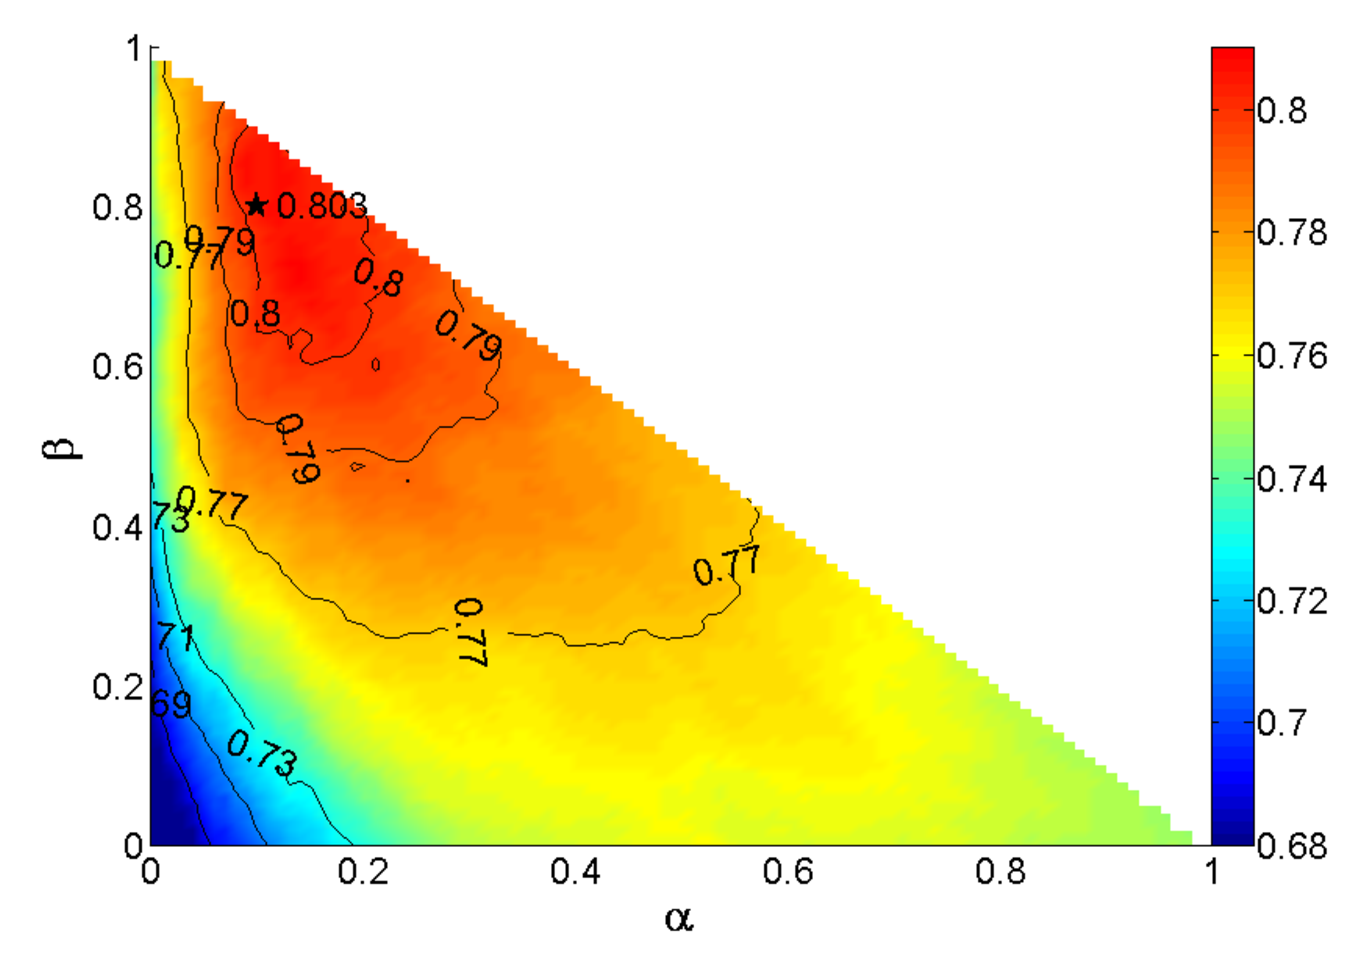
\includegraphics[scale=\graphscaleexpapp]{./exp/AAN-para-recm.eps}}
%\quad\quad
%\hspace{\graphmarginexpapp}
\hfill
\subfigure[{\scriptsize \aminer with \recom}]{\label{exp-aminer-ab-recom}
\includegraphics[scale=\graphscaleexpapp]{./exp/AMiner-para-recm.eps}}
%\quad\quad
%\hspace{\graphmarginexpapp}
\hfill
\subfigure[{\scriptsize \magdata with \recom}]{\label{exp-mag-ab-recom}
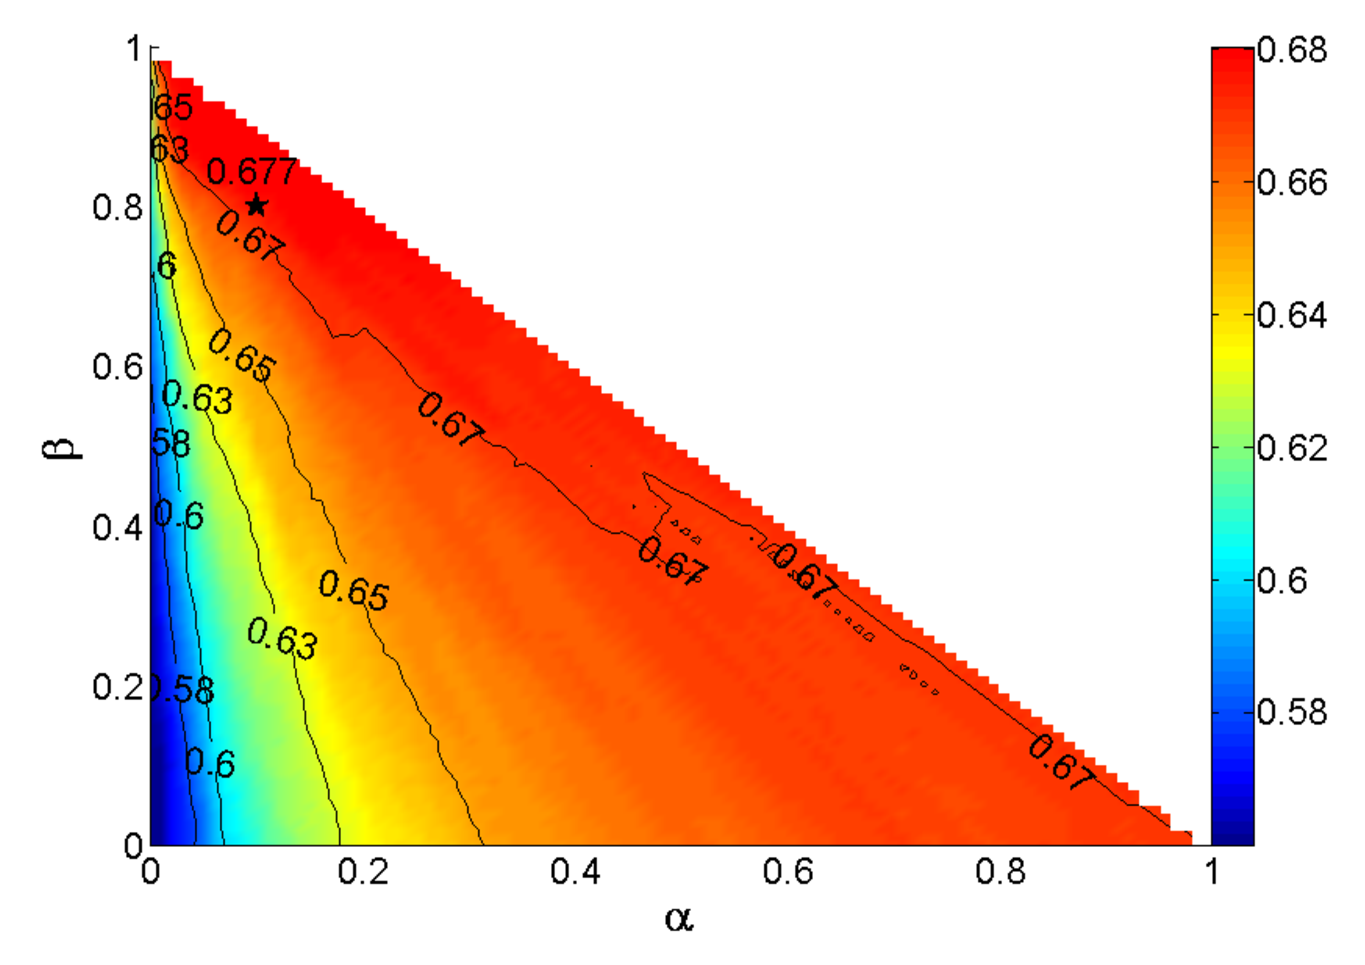
\includegraphics[scale=\graphscaleexpapp]{./exp/MAG-para-recm.eps}}
\\ %%%%%%%%%%%%%%%%%%%%%%%%%%%%%%%%%%%%%%
\vspace{-2ex}
%\hspace{-10ex}
\subfigure[{\scriptsize \aan  with \fcita}]{\label{exp-aan-ab-fcita}
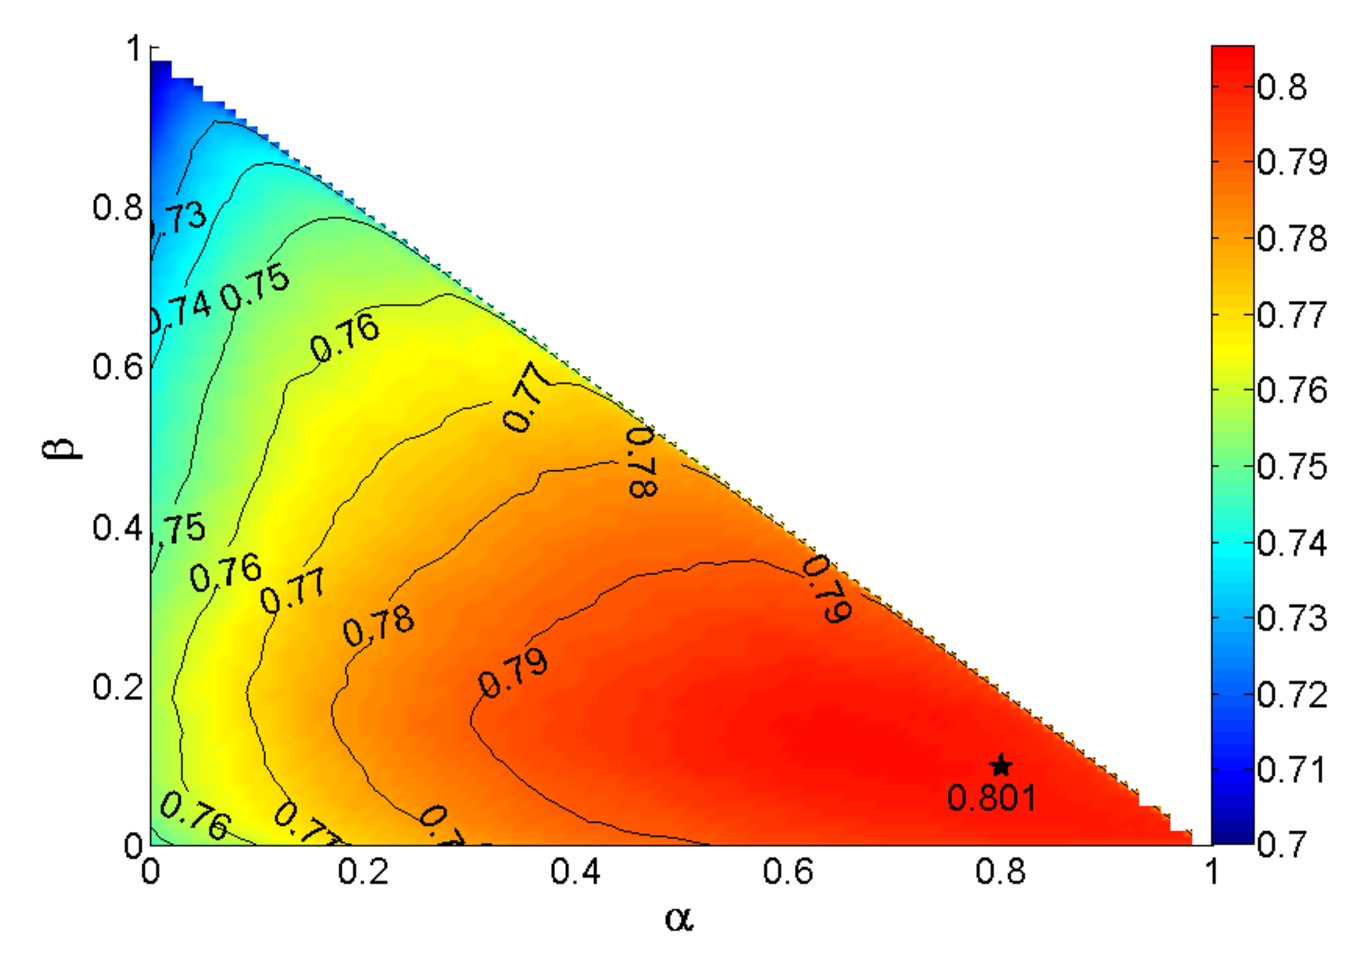
\includegraphics[scale=\graphscaleexpapp]{./exp/AAN-para-fcita.eps}}
%\quad\quad
%\hspace{\graphmarginexpapp}
\hfill
\subfigure[{\scriptsize \aminer with \fcita}]{\label{exp-aminer-ab-fcita}
\includegraphics[scale=\graphscaleexpapp]{./exp/AMiner-para-fcita.eps}}
%\quad\quad
%\hspace{\graphmarginexpapp}
\hfill
\subfigure[{\scriptsize \magdata with \fcita}]{\label{exp-mag-ab-fcita}
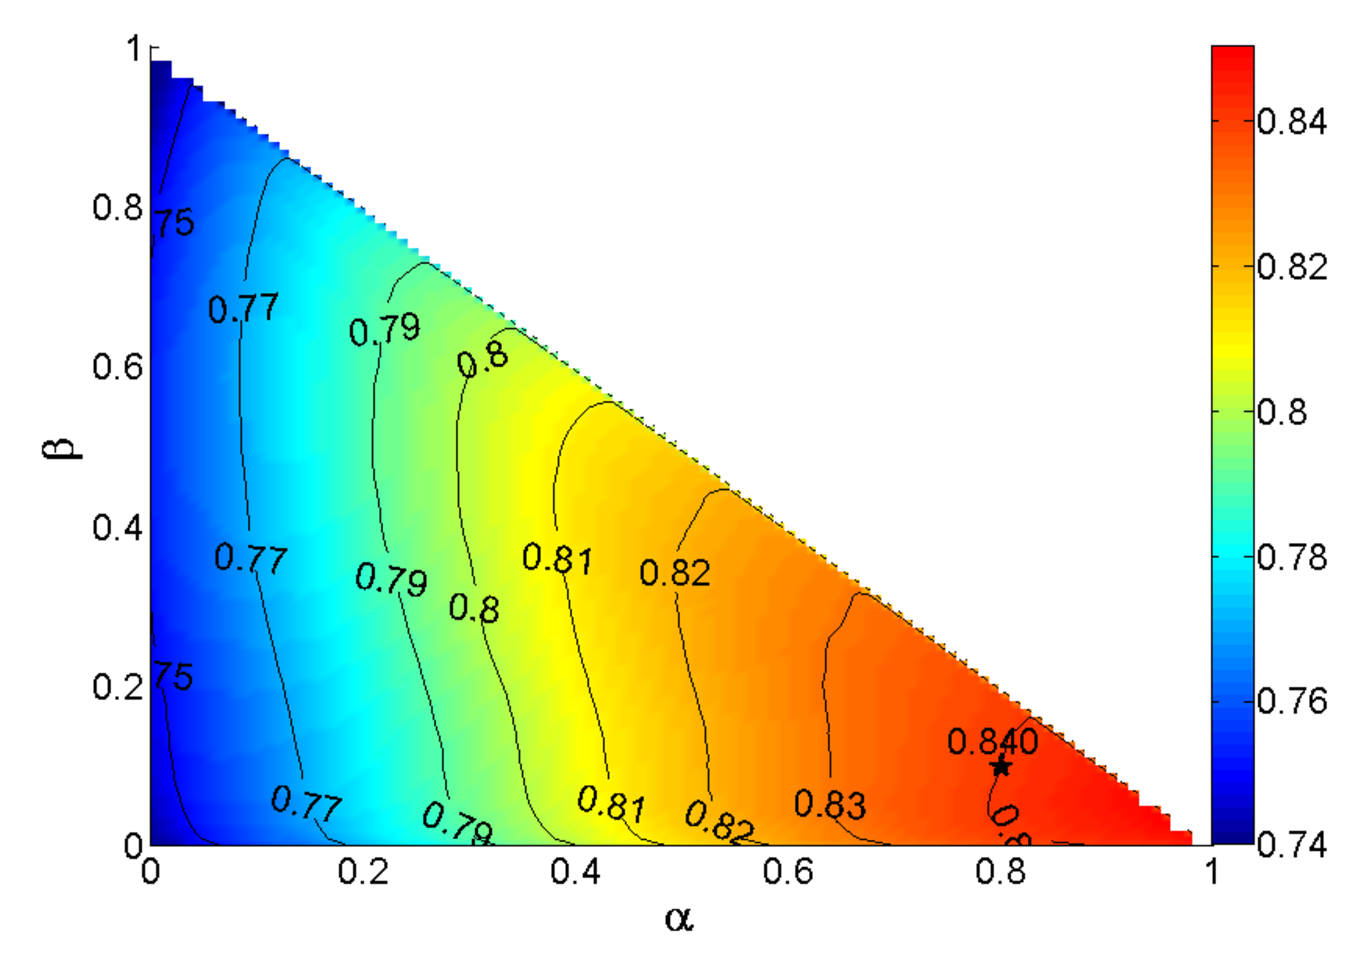
\includegraphics[scale=\graphscaleexpapp]{./exp/MAG-para-fcita.eps}}
\end{center}
\vspace{-2.5ex}
\caption{\small Accuracy tests: varying aggregating parameters $\alpha$ and $\beta$}
\label{exp-ab}
\vspace{-3ex}
\end{figure*}
%%%%%%%%%%%%%%%%%%%%%%%%%%%%%%%%%%%%%%

\stitle{Exp-4: Impacts of parameters}.
%\subsubsection{Exp-4: Impacts of parameters}.
In the last set of tests, we evaluated the impacts of time decaying factor $\sigma$, importance weighting factor $\lambda$, aggregating parameters $\alpha$ and $\beta$, and the TWPageRank. We fixed these parameters as well as $Y_s$ to their default values, used the TWPageRank proposed in this work by default, and tested the \PairAcc with the entire \recom and \fcita (\ie $T_i=+\infty$, $dif=1$).

%We present main results only and more details are available in~\cite{SARank-full}.




\etitle{Exp-4.1}.
%\stitle{Exp-4.1}.
To evaluate the impacts of the time decaying factor $\sigma$, we varied $\sigma$ from -1.6 to -0.4.
%, while fixed $Y_s$ to default values, $T_i=+\infty$, $dif=1$ and $\lambda=0.5$.
The results of \PairAcc are reported in Figs.~\ref{exp-aan-sigma}, \ref{exp-aminer-sigma} and \ref{exp-mag-sigma}.
%with both sets of ground-truth


When varying $\sigma$, the \PairAcc of \ensemblerank is very stable on all datasets using both \recom and \fcita. Indeed, with \recom and \fcita, the \PairAcc only varies (0.42\%, 1.55\%, 0.81\%) and (1.26\%, 0.96\%, 1.16\%) on (\aan, \aminer, \magdata), respectively.
%
%We omitted the detailed results of running time due to space constraint.
The running time varies (11.3\%, 8.6\%) on average only on (\aminer, \magdata), respectively.
%(0.18, 33.6) seconds, \ie

%Both of these show the robustness of \ensemblerank to the time decaying factor $\sigma$.

%As we can see from the figure, our method \ensemblerank is almost stable with the reduction of $\sigma$, since there is only a small fluctuation and the accuracy of our methods is always higher than the best baseline result in all datasets regardless of the change of $\sigma$. This means \ensemblerank is insensitive with $\sigma$.


%%%%%%%%%%%%%%%%%%%%%%%%%%%%%%%%%%%%%%%%%%%%%%%%%%
\begin{table}[tb!]
%\vspace{-2ex}
\begin{center}
\caption{\small Accuracy tests using different components with \recom (rows 2--4) and \fcita (rows 5--7).}
\label{tab-recom}
\begin{small}
\vspace{-.5ex}
\begin{tabular}{|c| c |c | c|}
\hline
{\bf Datasets} & {\bf C}\hspace{5ex}{\bf V}\hspace{5ex}{\bf A} & {\bf CV}\hspace{3ex}{\bf CA}\hspace{3ex}{\bf VA} & {\bf CVA} \\
\hline \hline
% \recom
\aan & 0.752 \ 0.616 \ 0.649 & 0.809 \ 0.764 \ 0.747 & {\bf 0.810} \\
\aminer & 0.735 \  0.581 \  0.640 & 0.784 \ 0.749 \ 0.729 & {\bf 0.785} \\
\magdata & 0.635 \ 0.534 \ 0.553 & 0.697 \ 0.673 \  0.648 & {\bf 0.698} \\ \hline
% \ficta
\aan & 0.785 \ 0.557 \ 0.761 & 0.849 \ 0.866 \ 0.771 & {\bf 0.870} \\
\aminer & 0.713 \  0.603 \  0.725 & 0.843 \ 0.847 \ 0.740 & {\bf 0.856} \\
\magdata & 0.736 \ 0.628 \ 0.718 & 0.848 \ 0.857 \ 0.751 & {\bf 0.874} \\
\hline
\end{tabular}
\end{small}
\end{center}
\vspace{-6ex}
\end{table}
%%%%%%%%%%%%%%%%%%%


\etitle{Exp-4.2}.
%\stitle{Exp-4.2}.
To evaluate the impacts of importance weighting factor $\lambda$, we varied $\lambda$ from 0 to 1.
%while fixed $Y_s$ to default values, $T_i=+\infty$, $dif=1$ and $\sigma=-1.0$.
The results of \PairAcc are reported in Figs.~\ref{exp-aan-lambda}, \ref{exp-aminer-lambda} and \ref{exp-mag-lambda}. Note that parameter $\lambda$ has no impacts on efficiency.
%with both sets of ground-truth

When varying $\lambda$, the \PairAcc of \ensemblerank first increases and then decreases on all datasets with both \fcita and \recom, except on \aminer with \recom.
%\marked{The value of $\lambda$ for \ensemblerank to achieve the best effectiveness is (0.6, 0, 0.2) and (0.6, 0.4, 0.1) on (\aan, \aminer, \magdata) with \recom and \fcita, respectively.}
This result indicates that combining prestige and popularity generally produces more robust results than using either of prestige and popularity.
Indeed, with \recom and \fcita, the \PairAcc of combining prestige and popularity is (10.2\%, 10.7\%, 5.5\%) and (8.0\%, 8.7\%, 9.0\%) higher than using prestige alone, and is (1.2\%, -0.1\%, 1.0\%) and (1.0\%, 1.0\%, 0.3\%) higher than using popularity alone on (\aan, \aminer, \magdata), respectively.


%The selection of $\lambda$ is influenced by ground-truth, such that the best $\lambda$ falls into $[xx,xx]$ and $[yy,yy]$ on \fcita and \recom, respectively. Moreover, equally weighting, \ie $\lambda=0.5$, is a good default setting when no query information is available in advance.
%Indeed, the best obtained \PairAcc using (\fcita, \recom) is only (0.10\%, 0.38\%), (0.04\%, 2.59\%) and (0.06\%, 0.91\%)  higher than the \PairAcc of equally weighting on \aan, \aminer and \magdata, respectively.





\etitle{Exp-4.3}.
To evaluate the impacts of aggregating parameters $\alpha$ and $\beta$, we varied $\alpha$ and $\beta$ at the granularity of 0.01. Again, parameters $\alpha$ and $\beta$ have few impacts on efficiency. The results are reported in Fig.~\ref{exp-ab}, where the parameters selected earlier and their corresponding \PairAcc are marked with $*$.

When varying $\alpha$ and $\beta$, the \PairAcc of \ensemblerank changes gently, as shown in Fig.~\ref{exp-ab}.
The optimal \PairAcc is obtained within a single region, rather than a complex collection of optimal regions.
%
Moreover, the \PairAcc keeps at a high level within a certain ($\alpha$, $\beta$) combination space around the optimal region, as shown in Fig.~\ref{exp-ab}.
%For instance, consider a square of length 0.3, which covers 8.5\% of the parameter combination space. The fraction of parameters such that the \PairAcc is no worse than 1\% of the corresponding \PairAcc with marker $*$ is (73\%, 94\%) on \aan, (96\%, 87\%) on \aminer and (83\%, 95\%) on \magdata, using (\recom, \fcita), respectively.
%
Further, the optimal parameters on the same sets of ground-truth are very similar for (\aan, \aminer and \magdata), indicating that the setting of $\alpha$ and $\beta$ can be easily transferred across different datasets.
To conclude, \ensemblerank is very robust to parameters $\alpha$ and $\beta$, and it is quite flexible for choosing proper values of parameters $\alpha$ and $\beta$.

Moreover, this enables to verify the effectiveness of importance assembling from different components, whose results are reported in Table~IV, in which letters C, V and A stand for citation, venue and author components, respectively.
The ranking based on all components consistently performs the best, using both \recom and \fcita, which justifies the use of importance assembling for ranking scholarly articles.
%which, using \recom and \fcita, improves the \PairAcc over using components (C, V, A, CV, CA, VA) by (5.77\%, 19.4\%, 16.1\%, 0.09\%, 4.59\%, 6.28\%) and (9.54\%, 23.7\%, 5.90\%, 2.50\%, 0.71\%, 4.79\%) on \aan, (6.94\%, 23.7\%, 14.4\%, 0.21\%, 1.56\%, 7.67\%) and (17.68\%, 12.4\%, 9.61\%, 0.33\%, 1.88\%, 6.34\%) on \aminer, and (6.29\%, 16.38\%, 14.45\%, 0.05\%, 2.43\%, 5.02\%) and (11.43\%, 19.2\%, 11.2\%, 1.44\%, 0.77\%, 9.62\%) on \magdata, respectively.


\eat{
\etitle{Exp-4.3}.
%\stitle{Exp-4.3}.
To evaluate the impacts of aggregating parameters $\alpha$ and $\beta$, we varied $\alpha$ and $\beta$ at the granularity of 0.01.
%while fixed $Y_s$ to default values, $T_i=+\infty$, $dif=1$, $\sigma=-1.0$ and $\lambda=0.5$.
Again, parameters $\alpha$ and $\beta$ have few impacts on efficiency. Due to space limitations, we only present the main results and more details are available at~\cite{SARank-full}.

Indeed, \ensemblerank is very robust to parameters $\alpha$ and $\beta$.
(a) When varying $\alpha$ and $\beta$, the \PairAcc of \ensemblerank changes gently. (b) \PairAcc also keeps at a high level within a certain ($\alpha$, $\beta$)  combination space. Finally, (c) the optimal parameters on the same set of ground-truth are very similar for \aan, \aminer and \magdata. That is, it is quite flexible for choosing proper values
of  parameters $\alpha$ and $\beta$.
} %%%%%%%% brief version of Exp-4.3

%%%%%%%%%%%%%%%%%%%%%%%%%%%%%%%%%%%%%%
\begin{figure*}[tb!]
%\vspace{1ex}
\addtolength{\subfigcapskip}{-1ex}
\begin{center}
\subfigure[{\scriptsize \aan with \recom}]{\label{exp-aan-recom-drank}
\includegraphics[scale=0.35]{./exp/AAN_TWPageRank_recom.eps}}
\hfill
%\hspace{\graphmarginexpapp}
\subfigure[{\scriptsize \aminer with \recom}]{\label{exp-aminer-recom-drank}
\includegraphics[scale=0.35]{./exp/AMiner_TWPageRank_recom.eps}}
\hfill
%\hspace{\graphmarginexpapp}
\subfigure[{\scriptsize \magdata with \recom}]{\label{exp-mag-recom-drank}
\includegraphics[scale=0.35]{./exp/MAG_TWPageRank_recom.eps}}
\\%%%%%%%%%%%%%%%%%%%%%%%%%%%%%%%%%%%%%%%%%%%
\vspace{-1.5ex}
\subfigure[{\scriptsize \aan with \fcita}]{\label{exp-aan-fcita-drank}
\includegraphics[scale=0.35]{./exp/AAN_TWPageRank_fcita.eps}}
\hfill
%\hspace{\graphmarginexpapp}
\subfigure[{\scriptsize \aminer with \fcita}]{\label{exp-aminer-fcita-drank}
\includegraphics[scale=0.35]{./exp/AMiner_TWPageRank_fcita.eps}}
\hfill
%\hspace{\graphmarginexpapp}
\subfigure[{\scriptsize \magdata with \fcita}]{\label{exp-mag-fcita-drank}
\includegraphics[scale=0.35]{./exp/MAG_TWPageRank_fcita.eps}}
\end{center}
\vspace{-2.5ex}
\caption{\small Impacts of the TWPageRank on accuracy: varying importance weighting
factor $\lambda$}
\label{exp-drank}
\vspace{-3ex}
\end{figure*}
%%%%%%%%%%%%%%%%%%%%%%%%%%%%%%%%%%

\newcommand{\drank}{\kw{DRank}}


\etitle{Exp-4.4}.
\marked{To evaluate the impacts of the proposed TWPageRank, we compared our approach \ensemblerank with an algorithm alternative (referred to as \drank) the same to \ensemblerank except exploiting exponentially decayed impact weights, \ie $w(u,v)=e^{\sigma(T_u-T_v)}$ in Eq.~(\ref{eq-infl-weights}).
%The two algorithms produce the same popularity while different prestige.
To better understand the impacts, we varied the importance weighting factor $\lambda$ from 0.1 to 1. Note that the ranking results are the same when $\lambda=0$ due to the same popularity computation. The results are reported in Fig.~\ref{exp-drank}, where the numbers represent the improvement of \PairAcc by \ensemblerank over the one by \drank.}

\marked{
When varying $\lambda$, the \PairAcc of \ensemblerank is better than the one of \drank in most cases, which shows the superiority of the TWPageRank than exploiting exponentially decayed weights.
The difference of \PairAcc by the two algorithms is higher with \recom than with \fcita, since the two algorithms are using citation information to predict past and future citations with \fcita.
Moreover, algorithm \ensemblerank is consistently better than \drank when $0.5 \le \lambda \le 0.9$.
%, which, with \recom and \fcita, improves the \PairAcc by (2.88\%, 3.91\%, 3.90\%) and (0.55\%, 0.50\%, 0.22\%) on (\aan, \aminer, \magdata) on average, respectively.
The improvement decreases with the decrease of $\lambda$ as the popularity dominates the ranking with small $\lambda$, and in some cases, \drank outperforms \ensemblerank. %as the prestige and popularity orders of article pairs are more diverse for \drank than \ensemblerank.
Overall, with \recom and \fcita, \ensemblerank improves the \PairAcc over \drank by (1.78\%, 3.07\%, 3.20\%) and (0.29\%, 0.48\%, 0.11\%) on (\aan, \aminer, \magdata) on average, respectively.
}

\marked{
The TWPageRank has little impacts on efficiency, and the running time of the two algorithms only varies (6.34\%, 4.83\%) on (\aminer, \magdata) on average, respectively.}

\eat{
With the increment of $\lambda$, \ensemblerank has more promotion than DRank and the \PairAcc of DRank is better than \ensemblerank with small $\lambda$, possibly due to the addition of popularity will correct the mistaken pairs better on DRank, although \ensemblerank rank more pairs correctly.
In addition, the change of \PairAcc with \recom is higher than the one with \fcita, possibly due to the article pairs in \fcita are of the same years.
Moreover, the \PairAcc of \ensemblerank is better than its counterparts from $\lambda=0.5$ to $\lambda=1$, except on \aminer with \fcita. Recall that in Fig.~\ref{exp-aminer-lambda} using popularity alone gives the best results on \aminer, indicating that the prestige computed by TWPageRank is less accurate on \aminer than on the other two datasets.
%
Indeed, with \recom and \fcita, the \PairAcc of \ensemblerank is (2.20\%, 6.63\%, 5.68\%) and (0.25\%, 0.05\%, 0.05\%) higher than DRank on (\aan, \aminer, \magdata), respectively, when using prestige alone, and is (1.73\%, 2.97\%, 2.92\%) and (0.22\%, -0.08\%, 0.17\%) higher when combining prestige and popularity, respectively, on average.
%
Finally, the TWPageRank has little impacts on efficiency, and the running time of \ensemblerank and its counterparts only changes (6.34\%, 4.83\%) on (\aminer, \magdata) on average, respectively.
}

\stitle{Summary}.
From these tests we find the followings.


\sstab(1) Our model \ensemblerank is effective for ranking scholarly articles, which is consistently better than competitive methods in all tests. With \recom and \fcita, \ensemblerank improves \PairAcc over (\pagerank, \futurerank, \hhgrank) by
(13.5\%, 6.8\%, 4.8\%) and (12.0\%, 3.0\%, 3.2\%) on \aan,
(12.7\%, 5.0\%, 4.9\%) and (14.0\%, 6.5\%, 4.6\%) on \aminer, and
(6.5\%, 2.5\%, 2.2\%) and (13.4\%, 6.0\%, 2.4\%) on \magdata, on average, respectively.
%, and it has a great advantage in evaluating the importance in a long term. Furthermore, it is more accurate evaluating articles which have just published and is in lack of citations, since it uses both venue network and author information besides of citation network. Indeed, it improves the accuracy by $(7.9\%, 3.2\%, 2.3\%)$ and $(14.4\%, 5.0\%, 3.8\%)$ over \pagerank, \futurerank and \hhgrank on average of three datasets with recommendation based ground truth and future citation ground truth, respectively.


\sstab(2) Our batch algorithm \batensemble and incremental algorithm \incensemble are also efficient.
%
Our incremental algorithm \incensemble is on average (1.7, 3.1, 2.8, 117) and (2.0, 3.0, 4.4, 245) times faster than (\batensemble, \powensemble, \futurerank, \hhgrank)  on the large \aminer and \magdata, respectively.

%The batch algorithm \batensemble is on average (1.3, 2.5, 348) times faster than (\powensemble, \futurerank, \hhgrank)  on the largest \magdata, respectively.

%\noindent (3) Our incremental algorithms are much faster than their batch counterparts in practice, even their time complexity is very close. Indeed, algorithms \inctwprdag, \inctwprscc and \incensemble further improve the efficiency of (\twprdag, \twprscc, \batensemble) by (23\%, 38\%, 22\%) on average, respectively.


\sstab(3) Our ranking model \ensemblerank introduces the time decaying factor $\sigma$, importance weighting factor $\lambda$ and aggregating parameters $\alpha$ and $\beta$ for the sake of practicability and flexibility in real-life applications, and, from our tests, \ensemblerank is very robust to these parameters. Moreover, the proposed TWPageRank is generally more effective than directly using exponentially decayed impact weights.




\stitle{Related work}. We summarize related work as follows.
%
%Scholarly article ranking

Scholarly article ranking has shifted from citation count analysis~\cite{Garfield471,Hirsch15112005} to graph analysis~\cite{ChenXMR07,Zhou07-CoRank,Jiang12-MRank,Liang16AAAI,Li08TSRanking,Wang13AAAI,WalkerXKM07,sayyadi09,
Wang16TIST,Ng11KDD}.
Based on the information used, these methods are divided into four categories: (a) using the citation information only~\cite{Garfield471,Hirsch15112005,ChenXMR07,Ng11KDD}, (b) using the citation and temporal information~\cite{Li08TSRanking,WalkerXKM07}, (c) using the citation information and other heterogeneous information, \eg authors and venues of articles~\cite{Zhou07-CoRank,Jiang12-MRank,Liang16AAAI}, and (d) combining the citation, temporal and other heterogeneous information~\cite{sayyadi09,Wang16TIST,Wang13AAAI}.
Our work belongs to the last category aiming at fully employing information available for scholarly article ranking.


%\stitle{PageRank\&weighted PageRank algorithms}.

%PageRank \cite{Brin98:PageRank} and its extensions have been extensively used for citation analyses \cite{Waltman2014}. While PageRank equally propagates scores along outlinks, Weighted PageRank \cite{Xing04:WPR} extends PageRank by distributing scores based on the popularity of pages. Different from previous work, the Time-Weighted PageRank proposed in this work discriminately propagates scores in terms of citation statistics.

PageRank \cite{Brin98:PageRank} and its extensions have been extensively used for citation analyses \cite{Waltman2014}. While PageRank equally propagates scores along outlinks, Weighted PageRank extends PageRank by distributing scores based on certain criteria such as popularity of pages~\cite{Xing04:WPR} or authority of authors~\cite{Ding11}. Different from previous work, the Time-Weighted PageRank proposed in this work discriminately propagates scores in terms of citation statistics.






%\stitle{Dynamic algorithms}.

Dynamic algorithms have proven useful for various tasks by avoiding computing from scratch~\cite{RamalingamR93}.
% and only recomputing those affected by updates
%Dynamic algorithms have proven useful for graph analysis tasks, \eg incremental graph pattern matching~\cite{FanWW13} and  incremental simrank computation~\cite{YuLZ14}.
To our knowledge, little concern has been paid to dynamic scholarly article ranking except that~\cite{GhoshKHLL11} uses PageRank in dynamic citation networks. However, its solution is based on a strong and impractical assumption that there are no citations between articles in the same years.
Further, although there exist several studies on incremental PageRank computation~\cite{DesikanPSK05,AbiteboulPC03,WuR09} and on incremental PageRank approximation \cite{BahmaniCG10,BahmaniKMU12}, they are not designed for scholarly article ranking.
%
Different from previous work, we study scholarly article ranking in a dynamic environment in terms of
the citation characteristics of scholarly articles, which has never been exploited before.

%Our approach only makes the assumption that there are no mutual references within the citation network, which, we admit, violates xx\% of total citations on \magdata, and is significantly different (yy\% on \magdata) from~\cite{GhoshKHLL11}.  - move to Section 3

Ensemble methods use multiple learners to obtain better performance than could be obtained from a constituent learner alone~\cite{zhihua-book}.
%In this work, we leverage ensembles to produce better and robust results for scholarly article ranking~\cite{zhihua-book,wsdmcup,DuanAMHH16}.
In this work, we leverage  importance assembling  to produce better and robust results for scholarly article ranking~\cite{zhihua-book,wsdmcup,DuanAMHH16}.


\section{Conclusions}
\label{sec-conc}
We have proposed a model \ensemblerank for scholarly article ranking,
which assembles the importance of article, venue and author entities.
We have also proposed efficient batch and incremental algorithms for the computation of their importance, a combination of prestige and popularity.
As shown by the experimental study, our approach is both effective and efficient for scholarly article ranking.


A couple of topics need further investigation. First, we are to clean scholarly data with external data sources
\marked{and extend our model with affiliation and discipline information} for further improving the quality of ranking.
Second, we are to study distributed algorithms for importance computations, similar to \cite{ZhuYL05} that computes PageRank in distributed scenarios.

%A couple of topics need further investigation. First, we are to systematically study the impacts of different types of entities on the ranking of articles. Second, we are to evaluate the improvement of using external data.

%\newpage
\eat{
\begin{figure*}[tb!]
\vspace{-2ex}
\begin{minipage}[t]{0.5\textwidth}
\begin{center}
\subfigure[{\scriptsize TWPageRank (batch vs. inc.)}]{\label{fig-aminer-time2}
\includegraphics[scale=0.38]{./exp/AMiner_time_twpr.eps}}
%\quad\quad
\hspace{-0.5ex}
\subfigure[{\scriptsize Comparison of ranking algorithms}]{\label{fig-aminer-time1}
\includegraphics[scale=0.38]{./exp/AMiner_time.eps}}
\end{center}
\vspace{-5ex}
\caption{\small Efficiency tests on \aminer}
\label{fig-aminer-time}
\end{minipage}
\hspace{-2ex}
\begin{minipage}[t]{0.5\textwidth}
\begin{center}
\subfigure[{\scriptsize \aminer}]{\label{fig-aminer-time-sigma}
\includegraphics[scale=0.38]{./exp/AMiner_sigma_time.eps}}
%\quad\quad
\hspace{-0.5ex}
\subfigure[{\scriptsize \magdata}]{\label{fig-mag-time-sigma}
\includegraphics[scale=0.38]{./exp/MAG_sigma_time.eps}}
\end{center}
\vspace{-5ex}
\caption{\small Efficiency tests: varying $\sigma$}
\label{fig-time-sigma}
\end{minipage}
\vspace{-1ex}
\end{figure*}
}

\newcommand{\graphscaleexpapp}{0.262}
\newcommand{\graphmarginexpapp}{-2ex}
%%% all in 1 Figure
\begin{figure*}[tb!]
%\vspace{-2ex}
\begin{center}
%\hspace{-10ex}
\subfigure[{\scriptsize \aan}]{\label{fig-aan-ab-recom}
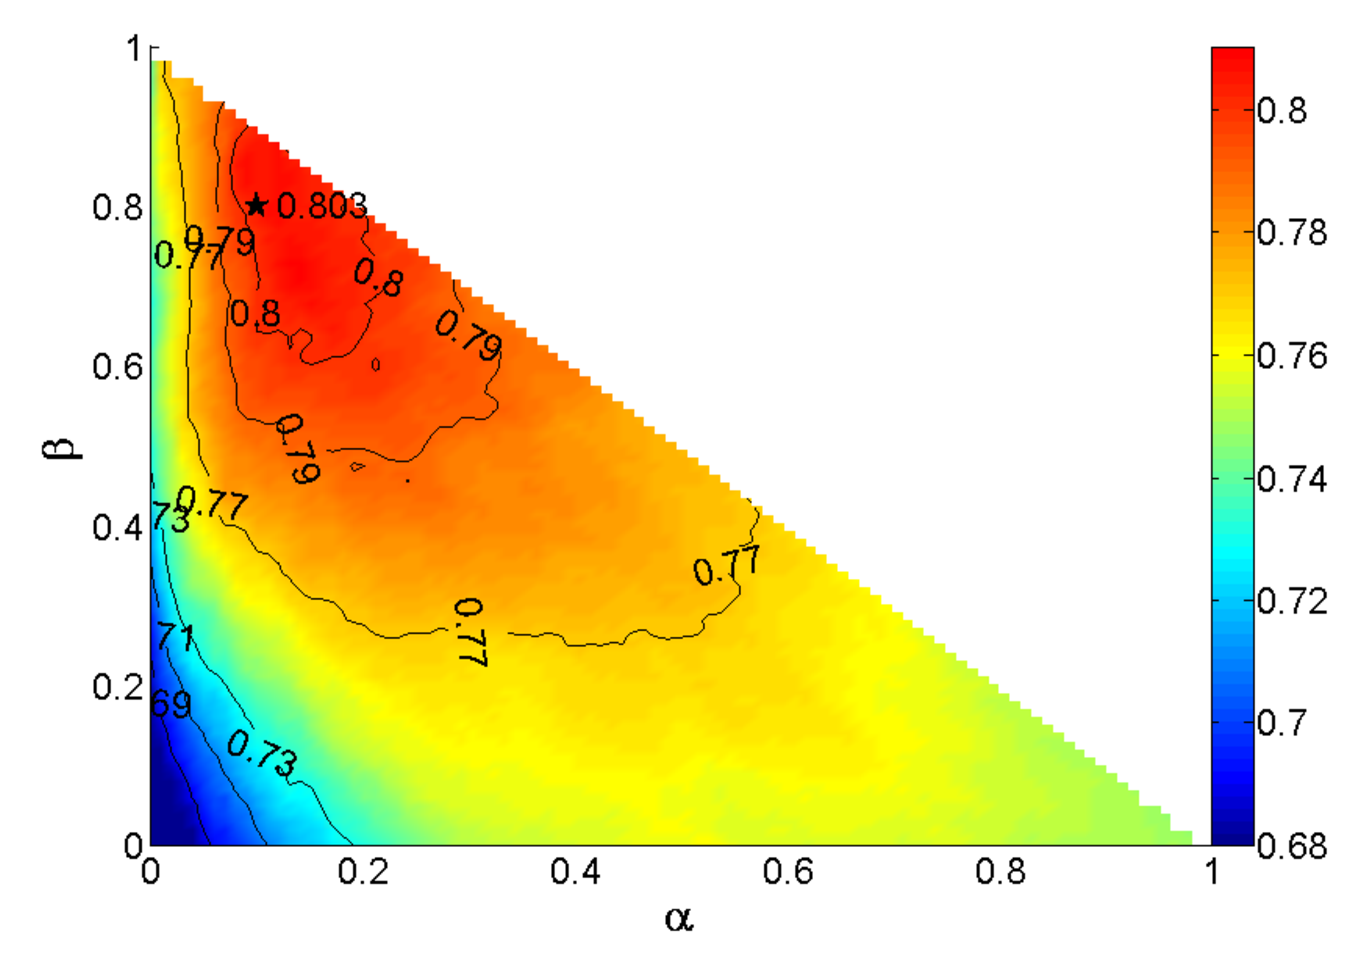
\includegraphics[scale=\graphscaleexpapp]{./exp/AAN-para-recm.eps}}
%\quad\quad
\hspace{\graphmarginexpapp}
\subfigure[{\scriptsize \aminer}]{\label{fig-aminer-ab-recom}
\includegraphics[scale=\graphscaleexpapp]{./exp/AMiner-para-recm.eps}}
%\quad\quad
\hspace{\graphmarginexpapp}
\subfigure[{\scriptsize \magdata}]{\label{fig-mag-ab-recom}
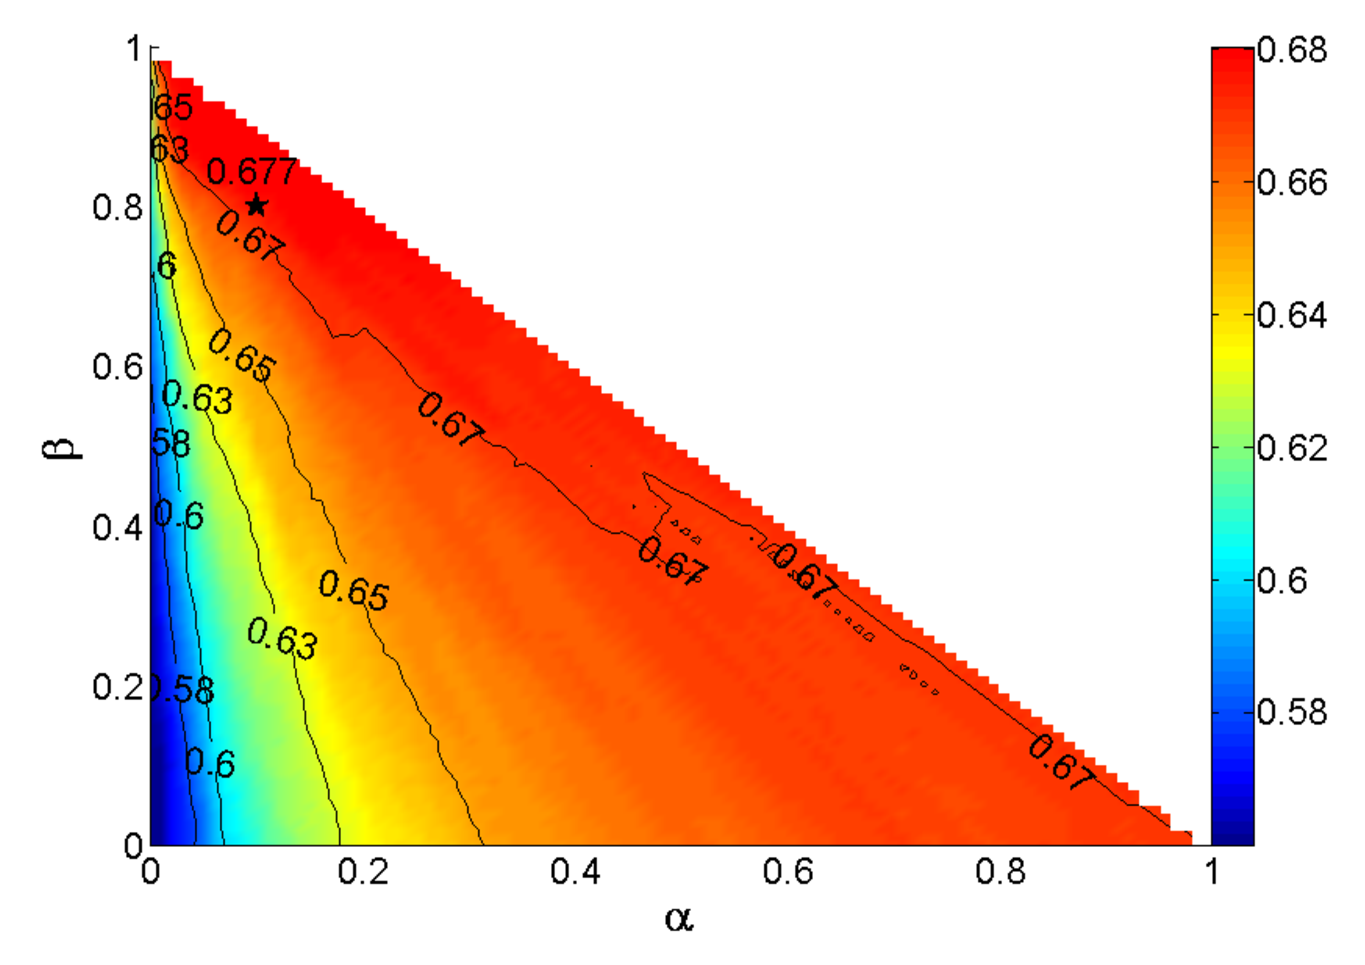
\includegraphics[scale=\graphscaleexpapp]{./exp/MAG-para-recm.eps}}
\\ %%%%%%%%%%%%%%%%%%%%%%%%%%%%%%%%%%%%%%
\vspace{-3ex}
%\hspace{-10ex}
\subfigure[{\scriptsize \aan}]{\label{fig-aan-ab-fcita}
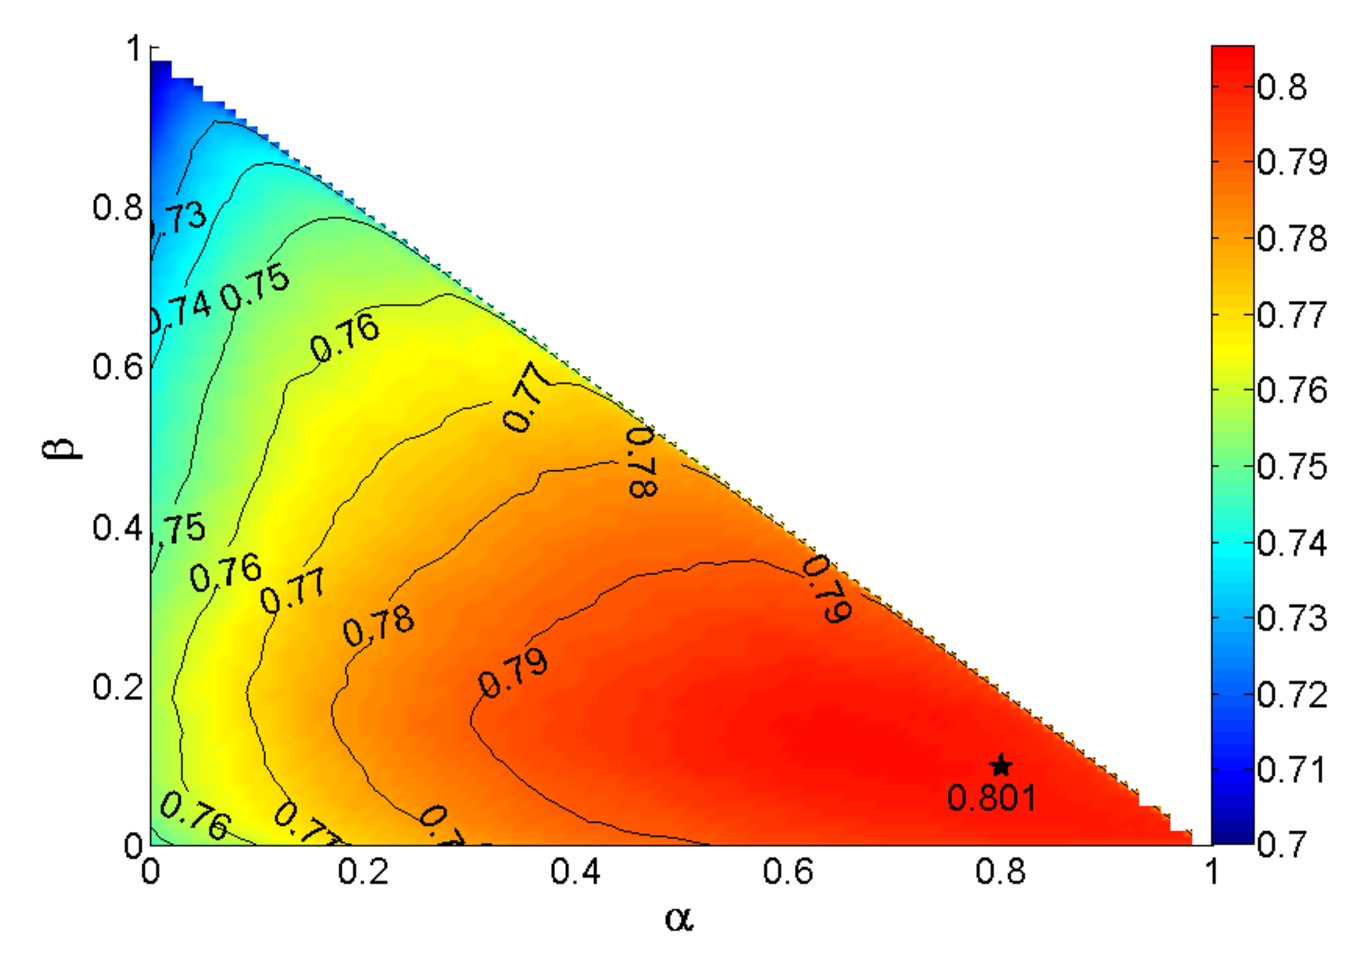
\includegraphics[scale=\graphscaleexpapp]{./exp/AAN-para-fcita.eps}}
%\quad\quad
\hspace{\graphmarginexpapp}
\subfigure[{\scriptsize \aminer}]{\label{fig-aminer-ab-fcita}
\includegraphics[scale=\graphscaleexpapp]{./exp/AMiner-para-fcita.eps}}
%\quad\quad
\hspace{\graphmarginexpapp}
\subfigure[{\scriptsize \magdata}]{\label{fig-mag-ab-fcita}
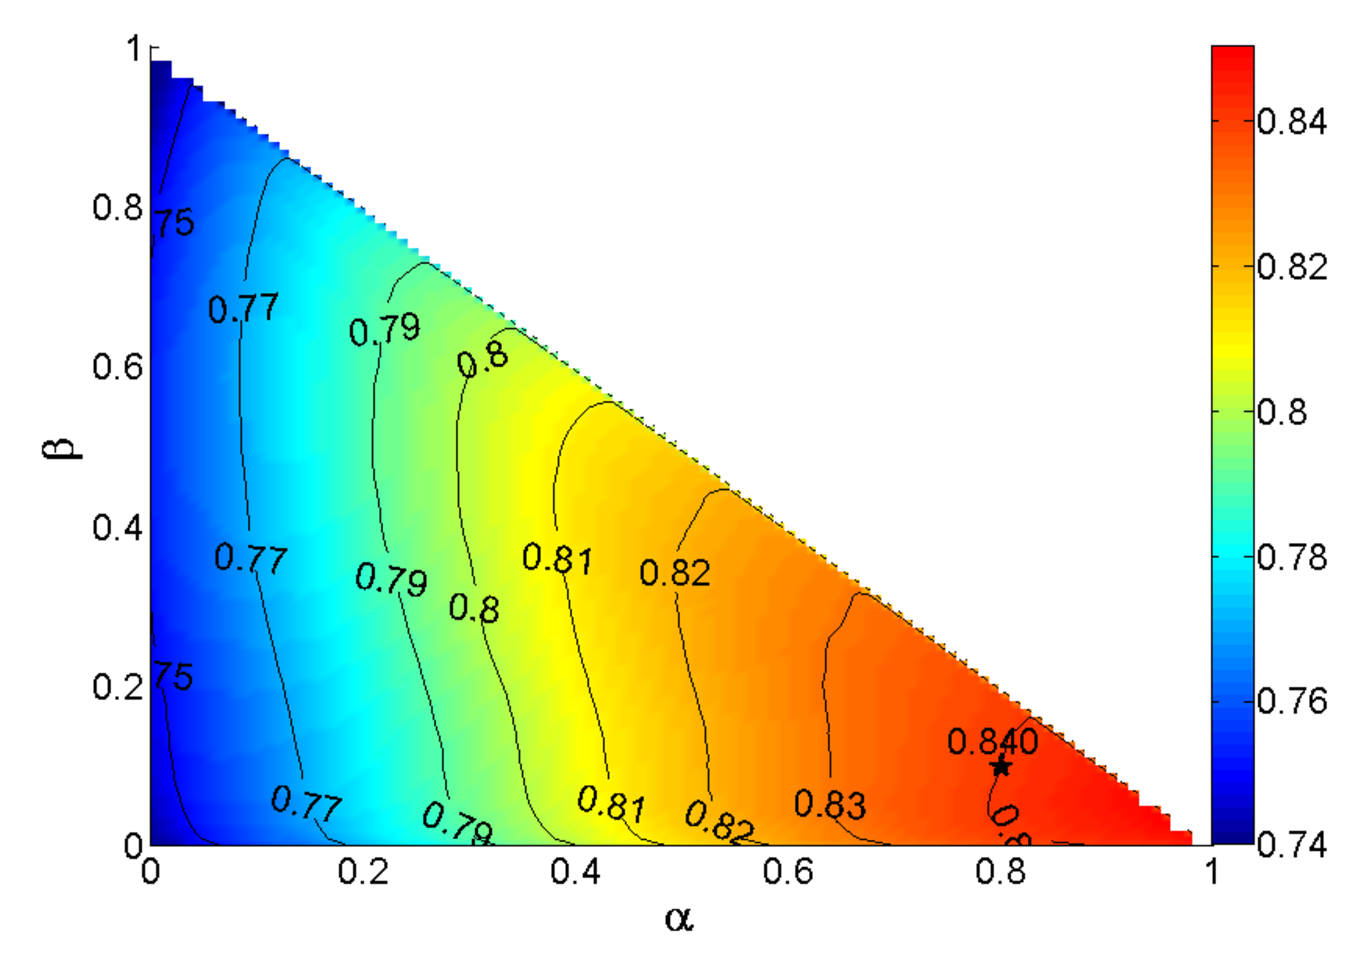
\includegraphics[scale=\graphscaleexpapp]{./exp/MAG-para-fcita.eps}}
\end{center}
\vspace{-5ex}
\caption{\small Accuracy tests with \recom ((a)--(c)) and \fcita ((d)--(f)): varying aggregating parameters $\alpha$ and $\beta$}
\label{fig-ab}
\vspace{-3ex}
\end{figure*}
%%%%%%%%%%%%%%%%%%%%%%%%%%%%%%%%%%%%%%

\vspace{-1ex}
\section*{APPENDIX A: Further Experiments}
\label{sec-exp-app}

\subsection*{1. Detailed results of Exp-4.3} %$\alpha$ and $\beta$ (detailed)

We present detailed results of {\em Exp-4.3}, which are omitted earlier due to the space constraints, \ie the impacts of aggregating parameters $\alpha$ and $\beta$ on effectiveness.

\eat{
\etitle{Exp-4.1}. To evaluate the impacts of the time decaying factor $\sigma$, we varied $\sigma$ from -1.6 to -0.4, while fixed $Y_s$ to default values, $b=+\infty$ and $dif=1$. The efficiency results are reported in Fig.~\ref{fig-time-sigma}.
Note that the running time of algorithm \batensemble is different on \recom and \fcita because of the different splitting year $Y_s$.

When varying $\sigma$, the running time of \batensemble is almost stable on both \aminer and \magdata using \fcita and \recom. Indeed, the running time using (\fcita, \recom) only varies (1.4\%, 0.5\%) on \aminer, and (2.1\%, 2.2\%) on \magdata, on average, respectively.
}

\etitle{Exp-4.3}.
To evaluate the impacts of parameters $\alpha$ and $\beta$ on effectiveness, we varied $\alpha$ and $\beta$ at the granularity of 0.01, while fixed $Y_s$ to default values, $b=+\infty$, $Dif=1$ and $\sigma=-1.0$. The results are reported in Fig.~\ref{fig-ab}, where the parameters selected earlier and their corresponding \PairAcc are marked with $*$.

When varying $\alpha$ and $\beta$, the \PairAcc of \ensemblerank changes gently, as shown in Fig.~\ref{fig-ab}.
The optimal \PairAcc is obtained within a single region, rather than a complex collection of optimal regions.
%
Moreover, the \PairAcc keeps at a high level within a certain ($\alpha$, $\beta$) combination space around the optimal region.
For instance, consider a square of length 0.3, which covers 8.5\% of the parameter combination space. The fraction of parameters such that the \PairAcc is no worse than 1\% of the corresponding \PairAcc with marker $*$ is (73\%, 94\%) on \aan, (96\%, 87\%) on \aminer and (83\%, 95\%) on \magdata, using (\recom, \fcita), respectively.
%
Further, the optimal parameters on the same benchmarks are very similar for (\aan, \aminer and \magdata), indicating that the setting of $\alpha$ and $\beta$ can be easily transferred across different datasets.
To conclude, \ensemblerank is very robust to parameters $\alpha$ and $\beta$, and it is quite flexible for choosing proper values of parameters $\alpha$ and $\beta$.

%For instance, consider a square of length 0.3, which covers 8.5\% of all parameter combinations.
%The fraction of parameters such that the \PairAcc is no worse than 1\% of the corresponding \PairAcc reported earlier is (73\%, 94\%) on \aan, (96\%, 87\%) on \aminer and (83\%, 95\%) on \magdata, using (\recom, \fcita), respectively. (See \cite{ERank-full} for complete results.)



\section*{APPENDIX B: Detailed Proofs}
\label{sec-proof}

\subsection*{1. Proof of Lemma \ref{prop-nonitercomputing}}

The TWPageRank vector $PR$ returned by \twprdag equals to the convergent TWPageRank vector $PR^*$.

\begin{proof}
We have $PR^* = d M^T\cdot PR^* + \frac{1-d}{n} e$, as $PR^*$ is the convergent TWPageRank vector. Hence, we also have
\begin{small}
\begin{equation}
PR^*(v)=d \sum_{(u,v)\in E^c} M_{u,v} PR^*(u) + \frac{1-d}{n}.
\end{equation}
\end{small}

\vspace{-1ex}
%\noindent

Consider a topological order $v_1/\dots/v_n$ on citation graph $G^c$. We then prove $PR(v_k)=PR^*(v_k)$ ($k\in[1,n]$) by induction.

\noindent(1) When $k=1$, it is obvious that $PR(v_k)=PR^*(v_k)=\frac{1-d}{n}$. %since $PR^*(v_1)=PR(v_1)=\frac{1-d}{n}$;

\noindent(2) Assume that it holds for $1\leq k \leq q$, we then show $PR^*(v_k)=PR(v_k)$ when $k=q+1$ as follows.
\begin{small}
\begin{equation*}
\begin{split}
PR^*(v_{q+1}) & = d \sum_u M_{u,v_{q+1}} PR^*(u) + \frac{1-d}{n} \\
 & = d \sum_u M_{u,v_{q+1}} PR(u) + \frac{1-d}{n}  = PR(v_{q+1}).
\end{split}
\end{equation*}
\end{small}

\vspace{-1ex}
\noindent Here $\{u|(u,v_{q+1})\in E^c\}\subseteq \{v_1,\dots,v_q\}$.
%By these, we have the conclusion.
\end{proof}







\subsection*{2. Proof of Proposition \ref{prop-prscc}}
The TWPageRank vector $PR$ returned by~\twprscc converges such that $||PR-PR^*||_1 < \epsilon$, where $PR^*$ is the convergent TWPageRank vector.

\begin{proof}
%By lemma~\ref{prop-converg}, we know that TWPageRank converges on venue graphs.
We first prove that the sum of changes after another iteration from $PR$ is smaller than $\epsilon$, \ie $||PR^+-PR||_1 < \epsilon$ where $PR^+=d M^T\cdot PR + \frac{1-d}{n} e$, and then prove that $||PR^*-PR||_1$ is smaller than the sum of changes.

Consider $scc_1$, $\dots$, $scc_m$ of the venue graph $G^v$ such that $v_1'/\dots$ $/v_m'$ is indeed a valid topological order of the converted $G'$ of $G^v$, where $m$ is the number of SCCs in $G^v$ and $v_k'$ ($k\in [1,m]$) is the corresponding nodes of $scc_k$ in $G'$.

Let $PR_k$ and $PR_k^-$ be the current and the previous TWPageRank vectors of nodes in $scc_k$ produced
by \twprscc, and $PR_k^+$ be the TWPageRank vector of nodes in $scc_k$ extracted from $PR^+$.
Further let $\Delta_k^-=PR_k-PR_k^-$ and we have:
$\sum_{k=1}^m ||\Delta_k^-||_1 < \epsilon$.

Consider $M_{ij}$ ($i,j\in[1,m]$), the transition submatrix from $scc_i$ to $scc_j$. We have $M_{ij}=\bf{0}$ when $i>j$, since there exists no edges from nodes in later $scc_i$ back to nodes in earlier $scc_j$. And, hence, $PR_k$ and $PR_k^+$ are updated as:
\vspace{-1ex}

\begin{small}
\begin{equation*}
\begin{split}
PR_k=&\frac{1-d}{n} e_k+ d \sum_{j=1}^{k-1} M_{jk}^T PR_j + d M_{kk}^T PR_k^-,\\
PR_k^+=&\frac{1-d}{n}  e_k+ d \sum_{j=1}^{k-1} M_{jk}^T PR_j + d M_{kk}^T PR_k,
\end{split}
\end{equation*}
\end{small}

\vspace{-1ex}
\noindent
respectively, where $e_k=[1]_{|scc_k|\times 1}$.
%, and, obviously, $\Delta_k^+=PR_k^+-PR_k=d M_{kk}^T \Delta_k^-$.

Hence, the sum of changes between $PR^+$ and $PR$ is:

\vspace{-1ex}
\begin{small}
\begin{equation*}
\begin{split}
||PR^+-PR||_1=&\sum_{k=1}^m ||PR_k^+-PR_k||_1=\sum_{k=1}^m ||d M_{kk}^T \Delta_k^-||_1 \\
\le & d\sum_{k=1}^m ||\Delta_k^-||_1 < \epsilon.
\end{split}
\end{equation*}
\end{small}

\vspace{-1ex}
\noindent
based on the fact that the row sums of $M_{kk}$ are always $\le 1$; %less than or equal to 1.

Moreover, $||PR^+-PR||_1 = ||PR^+ - PR^* + PR^* -PR||_1 = ||d M^T (PR-PR^*)||_1 + ||PR-PR^*||_1$, which gives $||PR-PR^*||_1<\epsilon$ and proves the conclusion.
\end{proof}


\subsection*{3. Proof of Proposition \ref{lemma-subgraphA}}
For nodes $v$ within $G^c_A$, $PR^+(v)= PR(v) {n}/{n^+}$.

\begin{proof}
Assume a topological order $v_1/\dots/v_{n_A}$ of graph $G^c_A$ with $n_A=|V^c_A|$.
We prove $PR^+(v_k)={n}/{n^+} PR(v_k)$ ($k\in [1,n_A]$) by induction.
%
Note that given $v\in V^c_A$, $\{(u,v)|(u,v)\in E^{c,+}\}=\{(u,v)|(u,v)\in E^c_A\}$, and, hence, $\Delta M_{u,v} =0$ for $(u,v)\in E^{c,+}$.

\noindent(1) When $k=1$, $PR^+(v_k)={n}/{n^+} PR(v_k)$ obviously holds since $\{(u,v_1)|(u,v_1)\in E^{c,+}\}=\emptyset$;

\noindent(2) Assume that it holds for $1\le k\le q$. We then show $PR^+(v_k)={n}/{n^+} PR(v_k)$ for $k=q+1$, since both ${(n^+-n)}/{n^+} PR(u) + \Delta PR(u)=0$ and $\Delta M_{u,v_{q+1}}=0$ when $(u,v_{q+1})\in E^{c,+}$.
Here $\{u|(u,v_{q+1})\in E^{c,+}\}\subseteq \{v_1,\dots,v_q\}$.
\end{proof}


\subsection*{4. A Stronger Convergence Result}

\eat{
\begin{proof}
%By lemma~\ref{prop-converg}, we know that TWPageRank converges on venue graphs.
It suffices to prove that the sum of changes of TWPageRank vector after another iteration is less than $\epsilon$, \ie $||PR^+-PR||_1 < \epsilon$ where $PR^+=d M^T PR + \frac{1-d}{n} e$.

Consider $scc_1$, $\dots$, $scc_m$ of $G$ such that their corresponding nodes $v_1'$, $\dots$, $v_m'$ are in the topological ordering of the converted DAG of $G$, where $m$ is the number of SCCs in $G$.
Let $PR_k$ and $PR_k^-$ (where $k\in\{1,\dots, m\}$) be the current and the previous TWPageRank vectors of nodes in $scc_k$ produced by \twprscc. Further let $\Delta_k^-=PR_k-PR_k^-$ and we have:
$\sum_{k=1}^m ||\Delta_k^-||_1 < \epsilon$.
Similarly, let $PR_k^+$ be the TWPageRank vectors of nodes in $scc_k$ extracted from $PR^+$.

Let $M_{ij}$ be the transition submatrix denoting the transition from $scc_i$ to $scc_j$, where $i,j\in \{1,\dots, m\}$. We have $M_{ij}=\bf{0}$ when $i>j$, since these exists no edges from later $scc_i$ back to early $scc_j$. And, hence, $PR_k$ and $PR_k^+$ are updated as:
\vspace{-1ex}

\begin{small}
\begin{equation*}
\begin{split}
PR_k=&\frac{1-d}{n}+ d \sum_{j=1}^{k-1} M_{jk}^T PR_j + d M_{kk}^T PR_k^-,\\
PR_k^+=&\frac{1-d}{n}+ d \sum_{j=1}^{k-1} M_{jk}^T PR_j + d M_{kk}^T PR_k,
\end{split}
\end{equation*}
\end{small}

\vspace{-1ex}
\noindent
respectively. Hence, $\Delta_k^+=PR_k^+-PR_k=d\cdot M_{kk}^T \Delta_k^-$.

The sum of changes between $PR^+$ and $PR$ is:

\vspace{-1ex}
\begin{small}
\begin{equation*}
\begin{split}
||PR^+-PR||_1=&\sum_{k=1}^m ||\Delta_k^+||_1=\sum_{k=1}^m ||d M_{kk}^T \Delta_k^-||_1 \\
\le & d\sum_{k=1}^m ||\Delta_k^-||_1 < \epsilon.
\end{split}
\end{equation*}
\end{small}

\vspace{-1ex}
\noindent
based on the fact that the row sums of $M_{kk}$ are always less than or equal to 1.
\end{proof}
}  %%%%% eat proof




\begin{figure}[tb!]
\centering
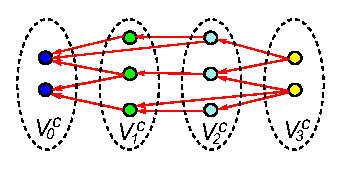
\includegraphics[scale=.8]{fig/DAG_Layers.eps}
\vspace{-2ex}
\caption{An example of a four-layer citation graph}
\label{fig-daglayers}
\vspace{-2ex}
\end{figure}


Proposotion~\ref{prop-converg} has shown the convergence of TWPageRank. We further present a stronger convergence result giving the number of iterations needed for power method to achieve convergence, which is based on dividing citation graphs into ordered layers.

Since the citation graph $G^c(V^c,E^c)$ can be treated as a directed acyclic graph, $V^c$ can be organized into ordered layers such that all edges are from later layers to earlier layers. To do this, let $l_v$ be the length of the longest path starting from node $v$,
%Such values for all nodes in $G$ can be computed in linear time~\cite{SedgewickW11}, by finding a topological ordering of $G$ and updating the length $l_v$ of each node $v$ in the topological ordering.
and $L$ be the length of the longest path starting from any node in $G^c$, \ie $L = \max_{v\in V^c} l_v$. Based on $l_v$,  $V^c$ is then divided into $L+1$ disjoint layers $V^c_0,V^c_1,\dots,V^c_{L}$ such that $V^c_0\bigcup V^c_1 \bigcup \dots \bigcup V^c_{L}=V^c$ and node $v\in V^c_{k}$ iff $l_v=k$. %($k\in[0,L]$).

\begin{example}
\label{eg-layer-dag}
Fig.~\ref{fig-daglayers} illustrates a four-layer citation graph, where $L$ equals to the length of the longest path, \ie 3, and the nodes are divided into 4 layers $[V^c_0, \ldots, V^c_3]$, such that $V^c_{k}$ ($k\in[0,3]$) contains all nodes starting from whom the length of the longest path is exactly $k$, and all edges are from  $V^c_i$ to $V^c_j$ where $i>j$.
\end{example}

\eat{
For the convenience of notation, we first rewrite the PageRank update rule in Eq.~(\ref{eq-twpr}) into matrix form:

\begin{small}
\begin{equation}
PR^{(t)}=d M^T \cdot PR^{(t-1)} + \frac{1-d}{n} e.
\end{equation}
\end{small}

\vspace{-1ex}
\noindent
Here $PR^{(t-1)}$ and $PR^{(t)}$ %, consisting of PageRank scores of all nodes,
are PageRank vectors after $t-1$ and $t$ iterations, respectively, $M$ is the transition matrix such that $M_{u,v}=w(u,v)/W(u)$ and $e$ is a $n$-dimentional vector $[1]_{n\times1}$.
}


\begin{prop} \label{prop-strong-conv}
TWPageRank converges to a unique vector on an $(L+1)$-layer citation graph after $L+1$ iterations, regardless of the initial vector.
\end{prop}

\begin{proof}
Given the initial TWPageRank vector $PR^{(0)}$, the PageRank vector after $t$ iterations is:
\vspace{-1ex}

\begin{small}
\begin{equation}
\label{eq-noniterpr}
%\begin{split}
PR^{(t)} =  d^t (M^T)^t PR^{(0)} + \frac{1-d}{n} \sum_{k=1}^{t-1}(d M^T)^k e +\frac{1-d}{n} e,
%\end{split}
\end{equation}
\end{small}

\vspace{-1ex}
\noindent
which is derived by iteratively computing $PR^{(1)}$ up to $PR^{(t)}$.

Without loss of generality, we consider $G^c$ whose nodes are properly arranged  such that nodes in $V^c_0$ come first, followed by ones in $V^c_1$ till $V^c_{L}$. In this case the transition matrix $M$ of $G^c$ is a strictly lower triangular matrix since all edges are from  $V^c_i$ to $V^c_j$ where $i>j$. Moreover, $M^{L+1}=\textbf{0}$.

When $t\ge L+1$, the first term in the right hand of Eq.~(\ref{eq-noniterpr}) becomes $\textbf{0}$, and $PR^{(t)}$ equals to
$\frac{1-d}{n} \sum_{k=1}^{L}(d M^T)^k e +\frac{1-d}{n} e$,
which is the unique convergent TWPageRank vector of $G^c$, regardless of the initial vector $PR^{(0)}$.
\end{proof}


\begin{figure*}[tb!]
%\vspace{-2ex}
\begin{center}
%\hspace{10ex}
\subfigure[{\scriptsize \aan)}]{\label{fig-aan-lambda}
\includegraphics[scale=0.38]{./exp/AAN_lambda.eps}}
%\quad\quad
\hspace{\graphmargin}
\subfigure[{\scriptsize \aminer}]{\label{fig-aminer-lambda}
\includegraphics[scale=0.38]{./exp/AMiner_lambda.eps}}
%\quad\quad
\hspace{\graphmargin}
\subfigure[{\scriptsize \magdata)}]{\label{fig-mag-lambda}
\includegraphics[scale=0.38]{./exp/MAG_lambda.eps}}
\end{center}
\vspace{-5ex}
\caption{\small Accuracy tests: varying importance weighting parameter $\lambda$}
\label{fig-lambda}
\vspace{-3ex}
\end{figure*}



\vspace{-1ex}
\section*{APPENDIX C: Further Experiments}
\label{sec-exp-app2}


\subsection*{1. Exp-5: Impacts of the importance weighting scheme on effectiveness}

Recall that the prestige and popularity are equally weighted to produce the importance by default in Eq.~(\ref{eq-imp}). In the fifth of tests, we further evaluated the impacts of the importance weighting scheme on effectiveness. To do this, we introduced the importance weighting parameter $\lambda$ such that $\lambda \in [0,1]$ and rewrote Eq.~(\ref{eq-imp}) as $Imp_c(v) = Prs_c(v)^\lambda \cdot Pop_c(v)^{1-\lambda}$, where $\lambda$ and $1-\lambda$ control the contributions of prestige and popularity to produce importance, respectively.
We varied $\lambda$ from 0 to 1, while fixed $Y_s$ to default values, $b=+\infty$, $dif=1$ and $\sigma=-1.0$. The results of the \PairAcc on both benchmarks are reported in Fig.~\ref{fig-lambda}. Note that parameter $\lambda$ has no impacts on efficiency.

When varying $\lambda$, the \PairAcc of \ensemblerank first increases and then decreases on all datasets using both benchmarks. This result indicated that our importance model combining both prestige and popularity is better than using either of prestige and popularity alone. The selection of $\lambda$ is influenced by benchmarks, such that the best $\lambda$ falls into $[xx,xx]$ and $[yy,yy]$ on \fcita and \recom, respectively. Moreover, equally weighting, \ie $\lambda=0.5$, is a good default setting when no query information is available in advance.
Indeed, the best obtained \PairAcc using (\fcita, \recom) is only (0.10\%, 0.38\%), (0.04\%, 2.59\%) and (0.06\%, 0.91\%)  higher than the \PairAcc of equally weighting on \aan, \aminer and \magdata, respectively. 


   %%use this one for appendix


\eat{%%%%%%%%%%%%EAT
\stitle{Acknowledgments}.
This work is supported in part by  973 program ({\small No. 2014CB340300}), NSFC ({\small No. 61322207\&61421003}),  Special Funds of Beijing Municipal Science \& Technology Commission, and MSRA Collaborative Research Program. We also thank Liang Duan, Niannian Wu and Dr. Xuelian Lin for their support.
}%%%%%%%%%%%%%%%%EAT


%
% The following two commands are all you need in the
% initial runs of your .tex file to
% produce the bibliography for the citations in your paper.

%\newpage
%\clearpage
\balance

\bibliographystyle{IEEEtran}
\begin{small}
\bibliography{paper}
\end{small}

%\bibliographystyle{ACM-Reference-Format}
%\bibliography{paper}

%APPENDICES are optional
%\balancecolumns

%\newpage
\eat{
\begin{figure*}[tb!]
\vspace{-2ex}
\begin{minipage}[t]{0.5\textwidth}
\begin{center}
\subfigure[{\scriptsize TWPageRank (batch vs. inc.)}]{\label{fig-aminer-time2}
\includegraphics[scale=0.38]{./exp/AMiner_time_twpr.eps}}
%\quad\quad
\hspace{-0.5ex}
\subfigure[{\scriptsize Comparison of ranking algorithms}]{\label{fig-aminer-time1}
\includegraphics[scale=0.38]{./exp/AMiner_time.eps}}
\end{center}
\vspace{-5ex}
\caption{\small Efficiency tests on \aminer}
\label{fig-aminer-time}
\end{minipage}
\hspace{-2ex}
\begin{minipage}[t]{0.5\textwidth}
\begin{center}
\subfigure[{\scriptsize \aminer}]{\label{fig-aminer-time-sigma}
\includegraphics[scale=0.38]{./exp/AMiner_sigma_time.eps}}
%\quad\quad
\hspace{-0.5ex}
\subfigure[{\scriptsize \magdata}]{\label{fig-mag-time-sigma}
\includegraphics[scale=0.38]{./exp/MAG_sigma_time.eps}}
\end{center}
\vspace{-5ex}
\caption{\small Efficiency tests: varying $\sigma$}
\label{fig-time-sigma}
\end{minipage}
\vspace{-1ex}
\end{figure*}
}

\newcommand{\graphscaleexpapp}{0.262}
\newcommand{\graphmarginexpapp}{-2ex}
%%% all in 1 Figure
\begin{figure*}[tb!]
%\vspace{-2ex}
\begin{center}
%\hspace{-10ex}
\subfigure[{\scriptsize \aan}]{\label{fig-aan-ab-recom}
\includegraphics[scale=\graphscaleexpapp]{./exp/AAN-para-recm.eps}}
%\quad\quad
\hspace{\graphmarginexpapp}
\subfigure[{\scriptsize \aminer}]{\label{fig-aminer-ab-recom}
\includegraphics[scale=\graphscaleexpapp]{./exp/AMiner-para-recm.eps}}
%\quad\quad
\hspace{\graphmarginexpapp}
\subfigure[{\scriptsize \magdata}]{\label{fig-mag-ab-recom}
\includegraphics[scale=\graphscaleexpapp]{./exp/MAG-para-recm.eps}}
\\ %%%%%%%%%%%%%%%%%%%%%%%%%%%%%%%%%%%%%%
\vspace{-3ex}
%\hspace{-10ex}
\subfigure[{\scriptsize \aan}]{\label{fig-aan-ab-fcita}
\includegraphics[scale=\graphscaleexpapp]{./exp/AAN-para-fcita.eps}}
%\quad\quad
\hspace{\graphmarginexpapp}
\subfigure[{\scriptsize \aminer}]{\label{fig-aminer-ab-fcita}
\includegraphics[scale=\graphscaleexpapp]{./exp/AMiner-para-fcita.eps}}
%\quad\quad
\hspace{\graphmarginexpapp}
\subfigure[{\scriptsize \magdata}]{\label{fig-mag-ab-fcita}
\includegraphics[scale=\graphscaleexpapp]{./exp/MAG-para-fcita.eps}}
\end{center}
\vspace{-5ex}
\caption{\small Accuracy tests with \recom ((a)--(c)) and \fcita ((d)--(f)): varying aggregating parameters $\alpha$ and $\beta$}
\label{fig-ab}
\vspace{-3ex}
\end{figure*}
%%%%%%%%%%%%%%%%%%%%%%%%%%%%%%%%%%%%%%

\vspace{-1ex}
\section*{APPENDIX A: Further Experiments}
\label{sec-exp-app}

\subsection*{1. Detailed results of Exp-4.3} %$\alpha$ and $\beta$ (detailed)

We present detailed results of {\em Exp-4.3}, which are omitted earlier due to the space constraints, \ie the impacts of aggregating parameters $\alpha$ and $\beta$ on effectiveness.

\eat{
\etitle{Exp-4.1}. To evaluate the impacts of the time decaying factor $\sigma$, we varied $\sigma$ from -1.6 to -0.4, while fixed $Y_s$ to default values, $b=+\infty$ and $dif=1$. The efficiency results are reported in Fig.~\ref{fig-time-sigma}.
Note that the running time of algorithm \batensemble is different on \recom and \fcita because of the different splitting year $Y_s$.

When varying $\sigma$, the running time of \batensemble is almost stable on both \aminer and \magdata using \fcita and \recom. Indeed, the running time using (\fcita, \recom) only varies (1.4\%, 0.5\%) on \aminer, and (2.1\%, 2.2\%) on \magdata, on average, respectively.
}

\etitle{Exp-4.3}.
To evaluate the impacts of parameters $\alpha$ and $\beta$ on effectiveness, we varied $\alpha$ and $\beta$ at the granularity of 0.01, while fixed $Y_s$ to default values, $b=+\infty$, $Dif=1$ and $\sigma=-1.0$. The results are reported in Fig.~\ref{fig-ab}, where the parameters selected earlier and their corresponding \PairAcc are marked with $*$.

When varying $\alpha$ and $\beta$, the \PairAcc of \ensemblerank changes gently, as shown in Fig.~\ref{fig-ab}.
The optimal \PairAcc is obtained within a single region, rather than a complex collection of optimal regions.
%
Moreover, the \PairAcc keeps at a high level within a certain ($\alpha$, $\beta$) combination space around the optimal region.
For instance, consider a square of length 0.3, which covers 8.5\% of the parameter combination space. The fraction of parameters such that the \PairAcc is no worse than 1\% of the corresponding \PairAcc with marker $*$ is (73\%, 94\%) on \aan, (96\%, 87\%) on \aminer and (83\%, 95\%) on \magdata, using (\recom, \fcita), respectively.
%
Further, the optimal parameters on the same benchmarks are very similar for (\aan, \aminer and \magdata), indicating that the setting of $\alpha$ and $\beta$ can be easily transferred across different datasets.
To conclude, \ensemblerank is very robust to parameters $\alpha$ and $\beta$, and it is quite flexible for choosing proper values of parameters $\alpha$ and $\beta$.

%For instance, consider a square of length 0.3, which covers 8.5\% of all parameter combinations.
%The fraction of parameters such that the \PairAcc is no worse than 1\% of the corresponding \PairAcc reported earlier is (73\%, 94\%) on \aan, (96\%, 87\%) on \aminer and (83\%, 95\%) on \magdata, using (\recom, \fcita), respectively. (See \cite{ERank-full} for complete results.)



\section*{APPENDIX B: Detailed Proofs}
\label{sec-proof}

\subsection*{1. Proof of Lemma \ref{prop-nonitercomputing}}

The TWPageRank vector $PR$ returned by \twprdag equals to the convergent TWPageRank vector $PR^*$.

\begin{proof}
We have $PR^* = d M^T\cdot PR^* + \frac{1-d}{n} e$, as $PR^*$ is the convergent TWPageRank vector. Hence, we also have
\begin{small}
\begin{equation}
PR^*(v)=d \sum_{(u,v)\in E^c} M_{u,v} PR^*(u) + \frac{1-d}{n}.
\end{equation}
\end{small}

\vspace{-1ex}
%\noindent

Consider a topological order $v_1/\dots/v_n$ on citation graph $G^c$. We then prove $PR(v_k)=PR^*(v_k)$ ($k\in[1,n]$) by induction.

\noindent(1) When $k=1$, it is obvious that $PR(v_k)=PR^*(v_k)=\frac{1-d}{n}$. %since $PR^*(v_1)=PR(v_1)=\frac{1-d}{n}$;

\noindent(2) Assume that it holds for $1\leq k \leq q$, we then show $PR^*(v_k)=PR(v_k)$ when $k=q+1$ as follows.
\begin{small}
\begin{equation*}
\begin{split}
PR^*(v_{q+1}) & = d \sum_u M_{u,v_{q+1}} PR^*(u) + \frac{1-d}{n} \\
 & = d \sum_u M_{u,v_{q+1}} PR(u) + \frac{1-d}{n}  = PR(v_{q+1}).
\end{split}
\end{equation*}
\end{small}

\vspace{-1ex}
\noindent Here $\{u|(u,v_{q+1})\in E^c\}\subseteq \{v_1,\dots,v_q\}$.
%By these, we have the conclusion.
\end{proof}







\subsection*{2. Proof of Proposition \ref{prop-prscc}}
The TWPageRank vector $PR$ returned by~\twprscc converges such that $||PR-PR^*||_1 < \epsilon$, where $PR^*$ is the convergent TWPageRank vector.

\begin{proof}
%By lemma~\ref{prop-converg}, we know that TWPageRank converges on venue graphs.
We first prove that the sum of changes after another iteration from $PR$ is smaller than $\epsilon$, \ie $||PR^+-PR||_1 < \epsilon$ where $PR^+=d M^T\cdot PR + \frac{1-d}{n} e$, and then prove that $||PR^*-PR||_1$ is smaller than the sum of changes.

Consider $scc_1$, $\dots$, $scc_m$ of the venue graph $G^v$ such that $v_1'/\dots$ $/v_m'$ is indeed a valid topological order of the converted $G'$ of $G^v$, where $m$ is the number of SCCs in $G^v$ and $v_k'$ ($k\in [1,m]$) is the corresponding nodes of $scc_k$ in $G'$.

Let $PR_k$ and $PR_k^-$ be the current and the previous TWPageRank vectors of nodes in $scc_k$ produced
by \twprscc, and $PR_k^+$ be the TWPageRank vector of nodes in $scc_k$ extracted from $PR^+$.
Further let $\Delta_k^-=PR_k-PR_k^-$ and we have:
$\sum_{k=1}^m ||\Delta_k^-||_1 < \epsilon$.

Consider $M_{ij}$ ($i,j\in[1,m]$), the transition submatrix from $scc_i$ to $scc_j$. We have $M_{ij}=\bf{0}$ when $i>j$, since there exists no edges from nodes in later $scc_i$ back to nodes in earlier $scc_j$. And, hence, $PR_k$ and $PR_k^+$ are updated as:
\vspace{-1ex}

\begin{small}
\begin{equation*}
\begin{split}
PR_k=&\frac{1-d}{n} e_k+ d \sum_{j=1}^{k-1} M_{jk}^T PR_j + d M_{kk}^T PR_k^-,\\
PR_k^+=&\frac{1-d}{n}  e_k+ d \sum_{j=1}^{k-1} M_{jk}^T PR_j + d M_{kk}^T PR_k,
\end{split}
\end{equation*}
\end{small}

\vspace{-1ex}
\noindent
respectively, where $e_k=[1]_{|scc_k|\times 1}$.
%, and, obviously, $\Delta_k^+=PR_k^+-PR_k=d M_{kk}^T \Delta_k^-$.

Hence, the sum of changes between $PR^+$ and $PR$ is:

\vspace{-1ex}
\begin{small}
\begin{equation*}
\begin{split}
||PR^+-PR||_1=&\sum_{k=1}^m ||PR_k^+-PR_k||_1=\sum_{k=1}^m ||d M_{kk}^T \Delta_k^-||_1 \\
\le & d\sum_{k=1}^m ||\Delta_k^-||_1 < \epsilon.
\end{split}
\end{equation*}
\end{small}

\vspace{-1ex}
\noindent
based on the fact that the row sums of $M_{kk}$ are always $\le 1$; %less than or equal to 1.

Moreover, $||PR^+-PR||_1 = ||PR^+ - PR^* + PR^* -PR||_1 = ||d M^T (PR-PR^*)||_1 + ||PR-PR^*||_1$, which gives $||PR-PR^*||_1<\epsilon$ and proves the conclusion.
\end{proof}


\subsection*{3. Proof of Proposition \ref{lemma-subgraphA}}
For nodes $v$ within $G^c_A$, $PR^+(v)= PR(v) {n}/{n^+}$.

\begin{proof}
Assume a topological order $v_1/\dots/v_{n_A}$ of graph $G^c_A$ with $n_A=|V^c_A|$.
We prove $PR^+(v_k)={n}/{n^+} PR(v_k)$ ($k\in [1,n_A]$) by induction.
%
Note that given $v\in V^c_A$, $\{(u,v)|(u,v)\in E^{c,+}\}=\{(u,v)|(u,v)\in E^c_A\}$, and, hence, $\Delta M_{u,v} =0$ for $(u,v)\in E^{c,+}$.

\noindent(1) When $k=1$, $PR^+(v_k)={n}/{n^+} PR(v_k)$ obviously holds since $\{(u,v_1)|(u,v_1)\in E^{c,+}\}=\emptyset$;

\noindent(2) Assume that it holds for $1\le k\le q$. We then show $PR^+(v_k)={n}/{n^+} PR(v_k)$ for $k=q+1$, since both ${(n^+-n)}/{n^+} PR(u) + \Delta PR(u)=0$ and $\Delta M_{u,v_{q+1}}=0$ when $(u,v_{q+1})\in E^{c,+}$.
Here $\{u|(u,v_{q+1})\in E^{c,+}\}\subseteq \{v_1,\dots,v_q\}$.
\end{proof}


\subsection*{4. A Stronger Convergence Result}

\eat{
\begin{proof}
%By lemma~\ref{prop-converg}, we know that TWPageRank converges on venue graphs.
It suffices to prove that the sum of changes of TWPageRank vector after another iteration is less than $\epsilon$, \ie $||PR^+-PR||_1 < \epsilon$ where $PR^+=d M^T PR + \frac{1-d}{n} e$.

Consider $scc_1$, $\dots$, $scc_m$ of $G$ such that their corresponding nodes $v_1'$, $\dots$, $v_m'$ are in the topological ordering of the converted DAG of $G$, where $m$ is the number of SCCs in $G$.
Let $PR_k$ and $PR_k^-$ (where $k\in\{1,\dots, m\}$) be the current and the previous TWPageRank vectors of nodes in $scc_k$ produced by \twprscc. Further let $\Delta_k^-=PR_k-PR_k^-$ and we have:
$\sum_{k=1}^m ||\Delta_k^-||_1 < \epsilon$.
Similarly, let $PR_k^+$ be the TWPageRank vectors of nodes in $scc_k$ extracted from $PR^+$.

Let $M_{ij}$ be the transition submatrix denoting the transition from $scc_i$ to $scc_j$, where $i,j\in \{1,\dots, m\}$. We have $M_{ij}=\bf{0}$ when $i>j$, since these exists no edges from later $scc_i$ back to early $scc_j$. And, hence, $PR_k$ and $PR_k^+$ are updated as:
\vspace{-1ex}

\begin{small}
\begin{equation*}
\begin{split}
PR_k=&\frac{1-d}{n}+ d \sum_{j=1}^{k-1} M_{jk}^T PR_j + d M_{kk}^T PR_k^-,\\
PR_k^+=&\frac{1-d}{n}+ d \sum_{j=1}^{k-1} M_{jk}^T PR_j + d M_{kk}^T PR_k,
\end{split}
\end{equation*}
\end{small}

\vspace{-1ex}
\noindent
respectively. Hence, $\Delta_k^+=PR_k^+-PR_k=d\cdot M_{kk}^T \Delta_k^-$.

The sum of changes between $PR^+$ and $PR$ is:

\vspace{-1ex}
\begin{small}
\begin{equation*}
\begin{split}
||PR^+-PR||_1=&\sum_{k=1}^m ||\Delta_k^+||_1=\sum_{k=1}^m ||d M_{kk}^T \Delta_k^-||_1 \\
\le & d\sum_{k=1}^m ||\Delta_k^-||_1 < \epsilon.
\end{split}
\end{equation*}
\end{small}

\vspace{-1ex}
\noindent
based on the fact that the row sums of $M_{kk}$ are always less than or equal to 1.
\end{proof}
}  %%%%% eat proof




\begin{figure}[tb!]
\centering
\includegraphics[scale=.8]{fig/DAG_Layers.eps}
\vspace{-2ex}
\caption{An example of a four-layer citation graph}
\label{fig-daglayers}
\vspace{-2ex}
\end{figure}


Proposotion~\ref{prop-converg} has shown the convergence of TWPageRank. We further present a stronger convergence result giving the number of iterations needed for power method to achieve convergence, which is based on dividing citation graphs into ordered layers.

Since the citation graph $G^c(V^c,E^c)$ can be treated as a directed acyclic graph, $V^c$ can be organized into ordered layers such that all edges are from later layers to earlier layers. To do this, let $l_v$ be the length of the longest path starting from node $v$,
%Such values for all nodes in $G$ can be computed in linear time~\cite{SedgewickW11}, by finding a topological ordering of $G$ and updating the length $l_v$ of each node $v$ in the topological ordering.
and $L$ be the length of the longest path starting from any node in $G^c$, \ie $L = \max_{v\in V^c} l_v$. Based on $l_v$,  $V^c$ is then divided into $L+1$ disjoint layers $V^c_0,V^c_1,\dots,V^c_{L}$ such that $V^c_0\bigcup V^c_1 \bigcup \dots \bigcup V^c_{L}=V^c$ and node $v\in V^c_{k}$ iff $l_v=k$. %($k\in[0,L]$).

\begin{example}
\label{eg-layer-dag}
Fig.~\ref{fig-daglayers} illustrates a four-layer citation graph, where $L$ equals to the length of the longest path, \ie 3, and the nodes are divided into 4 layers $[V^c_0, \ldots, V^c_3]$, such that $V^c_{k}$ ($k\in[0,3]$) contains all nodes starting from whom the length of the longest path is exactly $k$, and all edges are from  $V^c_i$ to $V^c_j$ where $i>j$.
\end{example}

\eat{
For the convenience of notation, we first rewrite the PageRank update rule in Eq.~(\ref{eq-twpr}) into matrix form:

\begin{small}
\begin{equation}
PR^{(t)}=d M^T \cdot PR^{(t-1)} + \frac{1-d}{n} e.
\end{equation}
\end{small}

\vspace{-1ex}
\noindent
Here $PR^{(t-1)}$ and $PR^{(t)}$ %, consisting of PageRank scores of all nodes,
are PageRank vectors after $t-1$ and $t$ iterations, respectively, $M$ is the transition matrix such that $M_{u,v}=w(u,v)/W(u)$ and $e$ is a $n$-dimentional vector $[1]_{n\times1}$.
}


\begin{prop} \label{prop-strong-conv}
TWPageRank converges to a unique vector on an $(L+1)$-layer citation graph after $L+1$ iterations, regardless of the initial vector.
\end{prop}

\begin{proof}
Given the initial TWPageRank vector $PR^{(0)}$, the PageRank vector after $t$ iterations is:
\vspace{-1ex}

\begin{small}
\begin{equation}
\label{eq-noniterpr}
%\begin{split}
PR^{(t)} =  d^t (M^T)^t PR^{(0)} + \frac{1-d}{n} \sum_{k=1}^{t-1}(d M^T)^k e +\frac{1-d}{n} e,
%\end{split}
\end{equation}
\end{small}

\vspace{-1ex}
\noindent
which is derived by iteratively computing $PR^{(1)}$ up to $PR^{(t)}$.

Without loss of generality, we consider $G^c$ whose nodes are properly arranged  such that nodes in $V^c_0$ come first, followed by ones in $V^c_1$ till $V^c_{L}$. In this case the transition matrix $M$ of $G^c$ is a strictly lower triangular matrix since all edges are from  $V^c_i$ to $V^c_j$ where $i>j$. Moreover, $M^{L+1}=\textbf{0}$.

When $t\ge L+1$, the first term in the right hand of Eq.~(\ref{eq-noniterpr}) becomes $\textbf{0}$, and $PR^{(t)}$ equals to
$\frac{1-d}{n} \sum_{k=1}^{L}(d M^T)^k e +\frac{1-d}{n} e$,
which is the unique convergent TWPageRank vector of $G^c$, regardless of the initial vector $PR^{(0)}$.
\end{proof}


\begin{figure*}[tb!]
%\vspace{-2ex}
\begin{center}
%\hspace{10ex}
\subfigure[{\scriptsize \aan)}]{\label{fig-aan-lambda}
\includegraphics[scale=0.38]{./exp/AAN_lambda.eps}}
%\quad\quad
\hspace{\graphmargin}
\subfigure[{\scriptsize \aminer}]{\label{fig-aminer-lambda}
\includegraphics[scale=0.38]{./exp/AMiner_lambda.eps}}
%\quad\quad
\hspace{\graphmargin}
\subfigure[{\scriptsize \magdata)}]{\label{fig-mag-lambda}
\includegraphics[scale=0.38]{./exp/MAG_lambda.eps}}
\end{center}
\vspace{-5ex}
\caption{\small Accuracy tests: varying importance weighting parameter $\lambda$}
\label{fig-lambda}
\vspace{-3ex}
\end{figure*}



\vspace{-1ex}
\section*{APPENDIX C: Further Experiments}
\label{sec-exp-app2}


\subsection*{1. Exp-5: Impacts of the importance weighting scheme on effectiveness}

Recall that the prestige and popularity are equally weighted to produce the importance by default in Eq.~(\ref{eq-imp}). In the fifth of tests, we further evaluated the impacts of the importance weighting scheme on effectiveness. To do this, we introduced the importance weighting parameter $\lambda$ such that $\lambda \in [0,1]$ and rewrote Eq.~(\ref{eq-imp}) as $Imp_c(v) = Prs_c(v)^\lambda \cdot Pop_c(v)^{1-\lambda}$, where $\lambda$ and $1-\lambda$ control the contributions of prestige and popularity to produce importance, respectively.
We varied $\lambda$ from 0 to 1, while fixed $Y_s$ to default values, $b=+\infty$, $dif=1$ and $\sigma=-1.0$. The results of the \PairAcc on both benchmarks are reported in Fig.~\ref{fig-lambda}. Note that parameter $\lambda$ has no impacts on efficiency.

When varying $\lambda$, the \PairAcc of \ensemblerank first increases and then decreases on all datasets using both benchmarks. This result indicated that our importance model combining both prestige and popularity is better than using either of prestige and popularity alone. The selection of $\lambda$ is influenced by benchmarks, such that the best $\lambda$ falls into $[xx,xx]$ and $[yy,yy]$ on \fcita and \recom, respectively. Moreover, equally weighting, \ie $\lambda=0.5$, is a good default setting when no query information is available in advance.
Indeed, the best obtained \PairAcc using (\fcita, \recom) is only (0.10\%, 0.38\%), (0.04\%, 2.59\%) and (0.06\%, 0.91\%)  higher than the \PairAcc of equally weighting on \aan, \aminer and \magdata, respectively. 


   %%use this one for appendix

\end{document}
